%%
%% This is file `sample-sigplan.tex',
%% generated with the docstrip utility.
%%
%% The original source files were:
%%
%% samples.dtx  (with options: `sigplan')
%% 
%% IMPORTANT NOTICE:
%% 
%% For the copyright see the source file.
%% 
%% Any modified versions of this file must be renamed
%% with new filenames distinct from sample-sigplan.tex.
%% 
%% For distribution of the original source see the terms
%% for copying and modification in the file samples.dtx.
%% 
%% This generated file may be distributed as long as the
%% original source files, as listed above, are part of the
%% same distribution. (The sources need not necessarily be
%% in the same archive or directory.)
%%
%% The first command in your LaTeX source must be the \documentclass command.
\documentclass[sigplan,screen]{acmart}

%%
%% \BibTeX command to typeset BibTeX logo in the docs
\AtBeginDocument{%
  \providecommand\BibTeX{{%
    \normalfont B\kern-0.5em{\scshape i\kern-0.25em b}\kern-0.8em\TeX}}}

\usepackage{amsmath}
\usepackage{amssymb}
\usepackage{graphicx}
\usepackage{subcaption}
\usepackage{cancel}
\usepackage{mathtools}
\usepackage{hyperref}
\usepackage{siunitx}
%\usepackage{subcaption}
\usepackage{float}
\usepackage{multirow}
\usepackage{verbatim}
\usepackage{algorithm}
\usepackage[noend]{algpseudocode}

%%
%% end of the preamble, start of the body of the document source.
\begin{document}

%%
%% The "title" command has an optional parameter,
%% allowing the author to define a "short title" to be used in page headers.
\title{Performance Benchmark of A Parallel Sparse Linear System Solver Using Conjugate Gradient}

%%
%% The "author" command and its associated commands are used to define
%% the authors and their affiliations.
%% Of note is the shared affiliation of the first two authors, and the
%% "authornote" and "authornotemark" commands
%% used to denote shared contribution to the research.
\author{Sushant Kumar}
\email{kumars12@rpi.edu}
\authornotemark[1]
\affiliation{%
	\institution{MSE, RPI}
	\streetaddress{110, 8th Street}
	\city{Troy}
	\state{New York}
	\postcode{12180}
}

\author{Narendra Nanal}
\email{nanaln@rpi.edu}
\authornotemark[2]
\affiliation{%
  \institution{MANE, RPI}
  \streetaddress{110, 8th Street}
  \city{Troy}
  \state{New York}
  \postcode{12180}
}

\author{Vignesh Vittal-Srinivasaragavan}
\email{vittav@rpi.edu}
\authornotemark[3]
\affiliation{%
	\institution{MANE, RPI}
	\streetaddress{110, 8th Street}
	\city{Troy}
	\state{New York}
	\postcode{12180}
}


%%
%% The abstract is a short summary of the work to be presented in the
%% article.
\begin{abstract}
  A clear and well-documented \LaTeX\ document is presented as an
  article formatted for publication by ACM in a conference proceedings
  or journal publication. Based on the ``acmart'' document class, this
  article presents and explains many of the common variations, as well
  as many of the formatting elements an author may use in the
  preparation of the documentation of their work.
\end{abstract}

\acmConference[Project]{}{Parallel Computing}{Spring '20}%


%%
%% Keywords. The author(s) should pick words that accurately describe
%% the work being presented. Separate the keywords with commas.
\keywords{datasets, neural networks, gaze detection, text tagging}

%%
%% This command processes the author and affiliation and title
%% information and builds the first part of the formatted document.
\maketitle

\section{Introduction}
Partial differential equations or PDEs can be used to describe phenomena such as heat diffusion, electrostatics, electrodynamics, fluid dynamics, elasticity, quantum mechanics etc. Tremendous efforts have been made over the years to solve theses equations numerically and simulate these phenomena. Finite difference, finite volume or finite element are some of the most popular methods. These methods discretize the domain into small parts and the governing equations are solved approximately. This leads to a system of linear equation. For large simulations, solving this system of equations is computationally most expensive operation. Parallel implementation of this operation can reduce the simulation time significantly. The objective of the project is to develop a parallel solver for system of linear equations using conjugate gradient algorithm and benchmark its performance for weak and strong scaling.

In this study we have created a conjugate gradient solver in C programming language which employs a \emph{Compressed Row Storage} (CRS) data-structure. The solver is parallelized using MPI and CUDA. We have considered a simple 1D heat equation problem which is solved using finite difference technique. By varying number of grid points we can get systems of linear equations of varying sizes. The performance of the solver is tested by running the only MPI version and hybrid CUDA/MPI version across multiple ranks. The rest of the report is organized as follows. In section 2 the conjugate gradient algorithm and the storage data structure is discussed. In section 3 the parallelization strategy for the solver is explained. Finally, in section 4 performance analysis of the solver is presented. 

\section{Conjugate Gradient Solver}
Solving PDEs numerically using finite difference or finite element technique leads to large system of matrix with sparse, symmetric and positive definite coefficient matrix. Conjugate gradient method \cite{conjugate} is suitable for solving such systems. The conjugate gradient algorithm and the corresponding storage data structure is explained in this section. 
\subsection{Conjugate Gradient Method}
Consider the following system of linear equations.
\begin{equation}
\textbf{Ax}=\textbf{b}
\end{equation}
Here, \textbf{A} is a known matrix of size $n\times n$. It symmetric, positive definite (i.e. $\textbf{x}^T\textbf{A}\textbf{x} >0$ for all non-zero vector $\textbf{x}$ in $\textbf{R}^n$). Vector \textbf{b} is known while \textbf{x} is a solution vector. Conjugate gradient method treats this as an optimization problem and finds the solution $\textbf{x}_*$ attractively. The objective function used in conjugate gradient method is as follows:
\begin{equation}\label{objective}
f(\textbf{x})= \frac{1}{2}\textbf{x}^T\textbf{A}\textbf{x}-\textbf{x}^T\textbf{b}
\end{equation}
Since matrix \textbf{A} is positive definite, the objective function given in the Eq. \eqref{objective} has a unique minimum. Considering the symmetric nature of matrix, the gradient of the given objective function can be calculated as follows:
\begin{equation}
\nabla f{\textbf{x}} = \textbf{Ax}-\textbf{b}
\end{equation}
Hence, optimum of the Eq. \eqref{objective} is the solution for the given system of linear equations.
Let $\textbf{P}=\{\textbf{p}_0, \textbf{p}_1, ....\textbf{p}_{(n-1)}\}$ be sequence of $n$ linearly independent directions. As $\textbf{P}$ forms basis in $R^n$, we can express the solution of the system $\textbf{x}_*$ as follows:
\begin{equation}
\textbf{x}_*= \textbf{x}_0 + \sum_{i=0}^{n-1}\alpha_i\textbf{p}_i
\end{equation}
Here, $\textbf{x}_0$ is the initial guess. This can be considered as finding the solution from an initial guess by taking steps in the sequence of $n$ linearly independent directions given by $P$. The step size for each direction is denoted by $\alpha$.\\
Given the initial guess $\textbf{x}_0$, the gradient at this point is $\textbf{Ax}_0-\textbf{b}$. According to steepest descent, the first step will be in the direction of negative gradient i.e. $\textbf{p}_0= \textbf{b}-\textbf{Ax}_0$. The new optimal location of \textbf{x} at any given $(k+1)$th step is given as:
\begin{equation}
\textbf{x}_{(k+1)}=\textbf{x}_k+\alpha_k\textbf{p}_k
\end{equation}
The conjugate gradient algorithm insists that directions $\textbf{P}$ are mutually orthogonal. This can be achieved by enforcing following condition: 
\begin{equation}
\textbf{p}_k= \textbf{r}_k-\sum_{i<k}\frac{\textbf{p}_i^{T}\textbf{A}\textbf{r}_k}{\textbf{p}_i^{T}\textbf{A}\textbf{p}_i}\textbf{p}_i
\end{equation}
Here, $\textbf{r}_k$ is the residual for the $k$th step given as $\textbf{r}_k=\textbf{b}-\textbf{Ax}_k$. The optimal step size $\alpha_k$ is give as:
\begin{equation}
\alpha_k=\frac{\textbf{p}^T_k\textbf{r}_k}{\textbf{p}^T_k\textbf{A}\textbf{p}_k}
\end{equation}
The resulting algorithm is as follows:

\begin{algorithm}
	\caption{Conjugate Gradient Method}
	\begin{algorithmic}[1]
		
		\State Initialize:
		\State $\textbf{r}_0 := \textbf{b}-\textbf{Ax}_0$
		\State $\textbf{p}_0 := \textbf{r}_0$
		\State $k := 0$
		
		\While{$\textbf{r}_{k+1} >$ tolerance} 
		\State $\alpha_k := \frac{\textbf{p}^T_k\textbf{r}_k}{\textbf{p}^T_k\textbf{A}\textbf{p}_k}$
		\State $\textbf{x}_{k+1} := \textbf{x}_k+\alpha_k\textbf{p}_k $
		\State $\textbf{r}_{k+1} := \textbf{x}_k-\alpha_k\textbf{A}\textbf{p}_k $
		\State $ \beta_k := \frac{\textbf{r}^T_{k+1}\textbf{r}_{k+1}}{\textbf{r}^T_{k}\textbf{r}_{k}}$
		\State $\textbf{p}_{k+1} := \textbf{r}_{k+1}+\beta_k\textbf{p}_k $
		\State $k := k+1$
		\EndWhile  
		\State Return: $\textbf{x}_{k+1}$    
		
	\end{algorithmic}
\end{algorithm}\label{algo}



\subsection{Compressed Row Storage Data-structure}\label{crs}
The coefficient matrix obtained from finite difference or finite element method is sparse in nature i.e. most of the entries in the matrix are zero. Number of non-zero entries in the sparse matrix varies from 4\% for larger systems to 25\% for smaller systems. In such cases storing all zero values can lead to excessive wastage of memory. This problem can be circumvented by using a special data-structure to store the matrix values. Compressed Row Storage (CRS) \cite{sparse} is a very popular data-structure used to store the sparse matrices efficiently. \\
In CRS data-structure a sparse matrix \textbf{M} of size $n\times n$ is stored using 3 one dimensional arrays. The array which stores non-zero entries in the matrix is denoted as $m\_vec$ while their corresponding column indices are stored in an array called $col\_index$. The third vector called here as $row\_index$ is used to extract row elements from $m\_vec$ vector. If the number of non-zero entries in the matrix is $nnz$ then $m\_vec$ and $col\_index$ has size $nnz$. The size of $row\_index$ is $(nnz+1)$ as one extra padding element is added for the first row. To extract $i$th row, first we calculate $row\_start=row\_index[i]$ and $row\_start=row\_index[i]$. The $i$th row elements are extracted by slicing $m\_vec$ starting from $row\_start$ and ending at $row\_end$. The number of non-zero entries in $i$th row is $(row\_end - row\_start)$. This process is explained using a following example. Consider a $4\times 4$ matrix:
\begin{align*}
\textbf{M} =
\begin{bmatrix}
0 & 0 & 0 & 0\\
5 & 8 & 0 & 0\\
0 & 0 & 3 & 0\\
0 & 6 & 0 & 0\\
\end{bmatrix}
\end{align*}
Using CRS data-structure matrix \textbf{M} is represented as follows:
\begin{align*}
m\_vec =
\begin{bmatrix}
5 & 8 & 3 & 6\\
\end{bmatrix}   \\
col\_index =
\begin{bmatrix}
0 & 1 & 2 & 1\\
\end{bmatrix}\\   
row\_index =
\begin{bmatrix}
0 & 0 & 2 & 3 & 4\\
\end{bmatrix}   
\end{align*}
To extract elements in the first row, $row\_start$ and $row\_end$ are calculated as follows:
\begin{align*}
row\_start = row\_index[1] = 0\\
row\_end = row\_index[2] = 2
\end{align*}
Using these indexes row elements are extracted as $m\_vec[0:2]=[5 \;\; 8]$ and the their corresponding column indices are $[0 \;\; 1]$. \\
The CRS data-structure does not make any assumptions about the sparsity pattern of the matrix. Buluc \textit{et al.} \cite{sparse2} have demonstrated efficiency of matrix-vector multiplication operation using CRS data-structure in parallel environment. All the operations presented in the algorithm \ref{algo} are performed on the three arrays used in the data-structure. 

\section{Parallel Conjugate Gradient Algorithm}
The conjugate gradient solver is implemented in parallel using both MPI and CUDA so that the solver can be run across multiple multiple processors and GPUs. In this section MPI and CUDA implementation of parallel algorithm is explained. We also discuss use of MPI I/O for reading and writing input/optupt files across different MPI ranks.

\subsection{MPI Implementation}
To implement the algorithm in parallel, the first step is to read data from an input file and distribute it across the processors. The obvious choice for data distribution is to divide the  coefficient matrix row wise. The coefficient matrix is divided into blocks based on the number of processors and each processor will be allocated with a particular block of rows. As explained in Section \ref{crs}, we use CRS data-structure to store the rows i.e. we only store non-zero elements in the row. Each processor will store the global row numbers allocated to it, non-zero elements in those rows and corresponding column indices. The matrix data-structure for an example matrix \textbf{M} (given in the Section \ref{crs}) using two processors is illustrated in Fig. \ref{fig1}.
\begin{figure}[h!]
	\begin{center}
		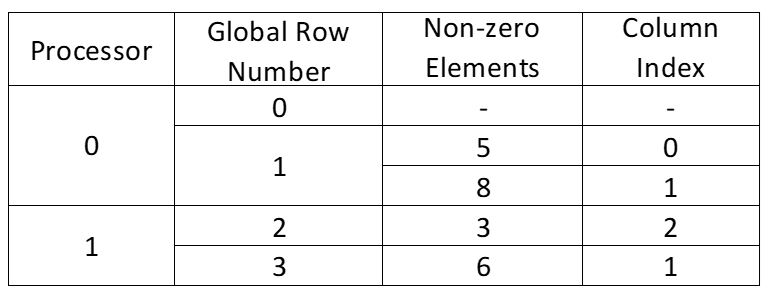
\includegraphics[width=0.4\textwidth]{plots/data.JPG}
	\end{center}
	\caption{Schematic representation of matrix data-structure for each processor}
	\label{fig1} 
\end{figure}
The solution vector \textbf{x} is stored completely on each processors.\\
The most time consuming linear algebra operations in the conjugate gradient algorithm are as follows:
\begin{enumerate}
	\item Matrix-vector multiplication
	\item Scaled Addition of two vectors
	\item Dot product of two vectors	
\end{enumerate}
Theses operations should be parallelized in an efficient way to get the maximum speedup.  The rest of the algorithm can be used unchanged.  
\subsubsection{Matrix-vector Multiplication}\label{mpi}
Matrix-vector multiplication is used to calculate the residual in the conjugate gradient algorithm. Consider a matrix-vector multiplication $\textbf{y}=\textbf{Ax}$. 
\begin{equation*}
\begin{bmatrix}
& & & & & \\
& & & & & \\
& & \mathbf{A}& & & \\
& & & & & \\
& & & & & \\
& & & & & 
\end{bmatrix}
\begin{Bmatrix}
\\
\\
\mathbf{x}\\
\\
\\
\\	
\end{Bmatrix}
= \begin{Bmatrix}
\\
\\
\mathbf{y}\\
\\
\\
\\	
\end{Bmatrix} 
\end{equation*}
The $i$th element in \textbf{y} can be expressed as:
\begin{equation}\label{eq1}
y_i= \textbf{A}_i\textbf{x}=\sum_{k=1}^{n}\textbf{A}_{i,k}\textbf{x}_k
\end{equation}
In CRS data-structure we only store non-zero elements and their corresponding column indices. Hence, the Eq. \ref{eq1} can be expressed as:
\begin{equation}
y_i = \sum_{k=1}^{nnz}\textbf{A}_{i,k}\textbf{x}_{c_k}
\end{equation}
Here, $c_k$ represents the column index for $k$th non-zero element in $i$th row. After parallelization the matrix vector product will be computed on different ranks as
\begin{equation*}
\begin{bmatrix}
\begin{bmatrix}
& & \mathbf{A}_1& & & \\
& & & & & \\
\end{bmatrix}\\
\hline\\
\begin{bmatrix}
& & \mathbf{A}_2& & & \\
& & & & & \\
\end{bmatrix}\\
\hline\\
\begin{bmatrix}
& & \mathbf{A}_3& & & \\
& & & & & \\
\end{bmatrix}\\
\end{bmatrix}
\begin{Bmatrix}
\\
\\
\\
\mathbf{x}\\
\\
\\
\\
\\	
\end{Bmatrix}
=\begin{Bmatrix}
\begin{Bmatrix}
\mathbf{y}_1\\
\\
\end{Bmatrix}\\
\hline\\
\begin{Bmatrix}
\mathbf{y}_2\\
\\
\end{Bmatrix}\\
\hline\\
\begin{Bmatrix}
\mathbf{y}_3\\
\\
\end{Bmatrix}	
\end{Bmatrix} 
\end{equation*}
In the above example, the serial matrix vector product is parallelized with 3 processors. Each processor handles a portion of the matrix  and multiplies it with full vector $\mathbf{x}$ to obtain the portion of the result vector. After the computation is completed by all the processors, all the locally computed elements are sent to all other processors. Better efficiency is achieved if the rows are distributed evenly across the processors.   

\subsubsection{Vector Addition}
Consider an addition of two vectors $\mathbf{x} + \mathbf{y} = \mathbf{z}$ i.e.
\begin{equation*}
\begin{Bmatrix}
\\
\\
\mathbf{x}\\
\\
\\
\\	
\end{Bmatrix} +
\begin{Bmatrix}
\\
\\
\mathbf{y}\\
\\
\\
\\	
\end{Bmatrix}
= \begin{Bmatrix}
\\
\\
\mathbf{z}\\
\\
\\
\\	
\end{Bmatrix}
\end{equation*}
Parallelizing the elementwise operations such as this with multiple processors very straightforward
\begin{equation*}
\begin{Bmatrix}
\begin{Bmatrix}
\mathbf{x}_1\\
\\
\end{Bmatrix}\\
\hline\\
\begin{Bmatrix}
\mathbf{x}_2\\
\\
\end{Bmatrix}\\
\hline\\
\begin{Bmatrix}
\mathbf{x}_3\\
\\
\end{Bmatrix}	
\end{Bmatrix} + 
\begin{Bmatrix}
\begin{Bmatrix}
\mathbf{y}_1\\
\\
\end{Bmatrix}\\
\hline\\
\begin{Bmatrix}
\mathbf{y}_2\\
\\
\end{Bmatrix}\\
\hline\\
\begin{Bmatrix}
\mathbf{y}_3\\
\\
\end{Bmatrix}	
\end{Bmatrix} = 
\begin{Bmatrix}
\begin{Bmatrix}
\mathbf{z}_1\\
\\
\end{Bmatrix}\\
\hline\\
\begin{Bmatrix}
\mathbf{z}_2\\
\\
\end{Bmatrix}\\
\hline\\
\begin{Bmatrix}
\mathbf{z}_3\\
\\
\end{Bmatrix}	
\end{Bmatrix}
\end{equation*}
Each processor will compute the sum of the specific set of rows which it operates on and will store the partial results in a local variable.

\subsubsection{Dot Product}
Dot product operation between two vectors is required for calculation of step size $\alpha$. The dot product between two vectors of size $n$ can be expressed as: $\textbf{x}.\textbf{y}=\sum_{i=1}^{n}\textbf{x}_i\textbf{y}_i$. 
\begin{equation*}
\begin{Bmatrix}
\\
\\
\mathbf{x}\\
\\
\\
\\	
\end{Bmatrix} \cdot
\begin{Bmatrix}
\\
\\
\mathbf{y}\\
\\
\\
\\	
\end{Bmatrix}
= sum\begin{Bmatrix}
\\
\\
\mathbf{x}\circ \mathbf{y}\\
\\
\\
\\	
\end{Bmatrix}
\end{equation*}

Both of the vectors are similarly distributed across the processors. Each processor calculates the partial dot product corresponding to its allocated elements as

\begin{equation*}
\begin{Bmatrix}
\begin{Bmatrix}
\mathbf{x}_1\\
\\
\end{Bmatrix}\\
\hline\\
\begin{Bmatrix}
\mathbf{x}_2\\
\\
\end{Bmatrix}\\
\hline\\
\begin{Bmatrix}
\mathbf{x}_3\\
\\
\end{Bmatrix}	
\end{Bmatrix} \cdot 
\begin{Bmatrix}
\begin{Bmatrix}
\mathbf{y}_1\\
\\
\end{Bmatrix}\\
\hline\\
\begin{Bmatrix}
\mathbf{y}_2\\
\\
\end{Bmatrix}\\
\hline\\
\begin{Bmatrix}
\mathbf{y}_3\\
\\
\end{Bmatrix}	
\end{Bmatrix} = 
sum\begin{Bmatrix}
sum\begin{Bmatrix}
\mathbf{x}_1 \circ \mathbf{y}_1\\
\\
\end{Bmatrix}\\
\hline\\
sum\begin{Bmatrix}
\mathbf{x}_2 \circ \mathbf{y}_2\\
\\
\end{Bmatrix}\\
\hline\\
sum\begin{Bmatrix}
\mathbf{x}_3 \circ \mathbf{y}_3\\
\\
\end{Bmatrix}	
\end{Bmatrix}
\end{equation*}


The partial dot product for $k$th processor can be expressed as follows:
\begin{equation}
s_k =\sum_{i=f_k}^{l_k}\textbf{x}_i\textbf{y}_i
\end{equation}
Here, $f_k$ and $l_k$ are respectively first and last indices of elements stored on $k$th processors. These partial dot products are  sent to the master processor using MPI\_Send and MPI\_Rec operations. The final dot product for $m$ processors is calculated on the mater processor as follows:
\begin{equation}
\textbf{x}.\textbf{y}= \sum_{k=1}^{m}s_k
\end{equation}
Finally, every processor requires a copy of complete dot product value for further operations. This achieved by MPI broadcast operation (MPI\_Bcast) where dot product value is sent to all the processors from master processor.

\subsection{CUDA Implementation}
Graphical Processing Unit (GPU) is a relatively new technology which has brought a paradigm shift in the field of high performance computing. It was originally developed for rendering graphics albeit over the years it has become indispensable for solving simulation problems hitherto considered computationally prohibitive. Here, we try to exploit the putative computational power of GPU programming for accelerating the performance of our conjugate gradient solver. The strength of GPUs predicates on the multitude of cores available for computation which empowers the user to run numerous threads concurrently without context switching. CUDA, which is a general purpose parallel computing platform and programming model developed by NVIDIA is commonly used for this purpose \cite{nvidia2011nvidia}.

However, GPU programming is not apt for every computational problem and it needs to be carefully evaluated as to how one could exploit the potential of this tool. Lee et al. have debunked the myth of the hundred-fold improvement in the performance of GPUs over CPUs through their expository work  \cite{lee2010debunking}. It was shown that intelligent optimization techniques could boost the performance of CPUs and deliver results at a speed comparable to GPUs. Karunadasa \& Ranasinghe \cite{karunadasa2009accelerating} implemented the Stranssen algorithm for matrix multiplication and conjugate gradient for solving a system of linear equations using a combination of MPI and CUDA. MPI was used to deliver data to the GPUs which in turn performed the computations to yield the final result. While significant improvement was observed in the performance of the Stranssen algorithm, the conjugate gradient algorithm failed to show an noteworthy speedup. The authors attributed this to a lack of second level of parallelism in the algorithm. However, certain application specific CUDA implementations of the conjugate gradient solver have yielded promising results. Maringnati et al \cite{maringanti2009acceleration} employed GPU programming for circuit simulation using a preconditioned conjugate gradient algorithm and found a speedup of upto 10 times relative to single-threaded CPU implementation. Zhang et al. \cite{zhang2013efficient} observed similar speedups for their implementation of a CUDA polynomial preconditioned conjugate gradient for elasticity related FEM problems. CUDA implementation for fluid flow problems has also bolstered the efficacy of the algorithm \cite{ji2012cuda, amador2010cuda}. Favorable performance in variegated areas  \cite{gravvanis2012solving,phillips2014cuda, li2014gpu, michels2011sparse, oyarzun2014mpi} has made the technique a hugely popular tool for numerical computing.

In contrast to the aforementioned CUDA implementations of conjugate gradient algorithm which make use of sophisticated tricks, we employ simpler techniques like reduction and seek to enhance the performance of the conjugate gradient algorithm used here. In the following section, we describe the algorithms we used for the CUDA implementation. 

\subsubsection{Matrix-vector implementation}

As explained in previous sections, we use the CSR data structure for representing the sparse matrices. Several pedagogical works have expounded the usage of CUDA for sparse matrix-vector product (SpMV) computation using this representation \cite{bell2008efficient, wang2010optimizing, spvm}. Figure \ref{spvm} illustrates how work is distributed for GPU computation of SpMV. This implementation functions at the level of rows per thread. As the kernel is launched, each thread computes the product corresponding to a single row of the sparse matrix. We use MPI to allocate a chunk of the full sparse matrix to a rank which is subsequently processed by the GPU threads. As a common practice in CUDA programming to make the code more portable, readable and scalable, one can also use grid-stride loops for parallelizing the loop using the kernel \cite{stride}. Schematically shown in Figure \ref{spvm}, this becomes imperative for solving problems on hardware where the thread grid is not large enough to cover the input array in entirety. 

\begin{figure}[h!]
	\begin{center}
		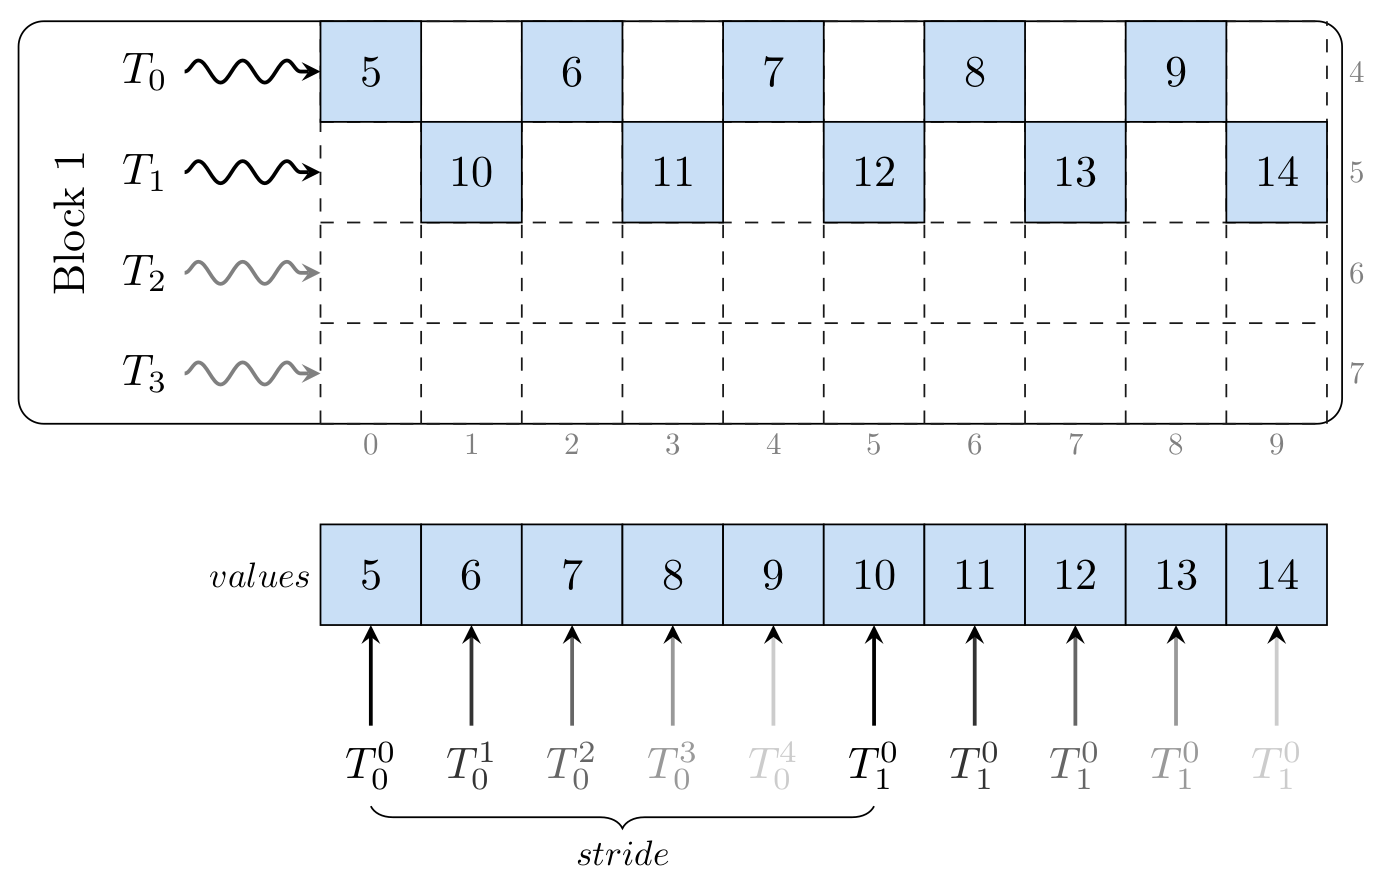
\includegraphics[width=0.45\textwidth]{plots/spvm.png}
	\end{center}
	\caption{Work distribution for SpMV implementation using CUDA \cite{spvm}}
	\label{spvm} 
\end{figure}

Nonetheless, issues of load balancing and thread divergence beset this simple and easy-to-understand algorithm for SpMV \cite{spvm}. The pattern of memory access which needlessly processes threads with zeros impinges upon the efficacy of this method. The performance of our code manifestly suffers due to this inefficiency and more sophisticated techniques like CSR-Vector reduction, CSR-Stream and CSR-Adaptive implementations are needed to observe significant speedups \cite{spvm}. 

\subsubsection{Vector dot product}\label{cuda_dot}

The algorithm, as implemented, needs to compute the dot product of multiple pairs of vectors on any given MPI rank. The concomitant computational load engenders the need to use GPU-enhanced processing of the dot product. A cursory glance at the problem suggests that CUDA is aptly suited for this job wherein each thread computes the product of the corresponding components of the vectors in parallel. However, calculating a vector dot product entails the reduction from vectors to a scalar.  
\begin{align}
c &= \vec{a} \cdot \vec{b} \\
&= (a_0,a_1,a_2,a_3)\cdot(b_0,b_1,b_2,b_3) \\
&= a_0b_0 + a_1b_1 + a_2b_2 + a_3b_3
\end{align}

To calculate the sum in the last equation, one could use different approaches. 

\begin{figure}[h!]
	\begin{center}
		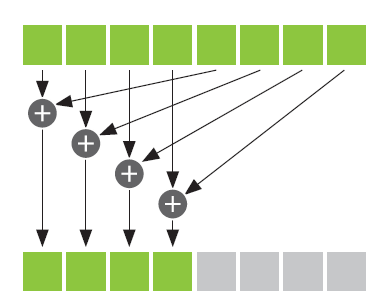
\includegraphics[width=0.45\textwidth]{plots/reduction.png}
	\end{center}
	\caption{Vector dot product: A step of summation reduction using CUDA \cite{spvm}}
	\label{spvm} 
\end{figure}




\subsection{MPI I/O}
MPI I/O modules are optimally implemented in the algorithm at three instances -- loading all partitioned input data in the right processor, load the full update vector on to each rank (after it is partially updated by each rank) and to write the partial final results from each rank to a common output file.

\subsubsection{Reading Partitioned Inputs}
The following binary files are required as inputs to solve the system of equations
\begin{enumerate}
	\item \texttt{Mvec} -- File which stores the sparse matrix as a vector
	\item \texttt{rowp} -- File storing the auxiliary array pointing to the index of first non-zero element of each row in \texttt{Mvec}
	\item \texttt{colm} -- File storing the column index of all non-zero entries
	\item \texttt{rhs} -- File storing the full RHS vector (i.e. $\mathbf{b}$ in $\mathbf{A}\mathbf{x}=\mathbf{b}$)
\end{enumerate} 

All the processors will have its own copy of the full RHS vector. The other 3 vectors are partitioned and read into each processor to ensure that values corresponding to the set of rows assigned to a processor are only read. 

The routine \texttt{MPI\_File\_read\_at()} is used to ensure that each process reads the right chunk of data from the input files and load them in relevant variables.

\subsubsection{Loading Update Vector}
The algorithm can be realized by using only one full-vector (i.e. a vector that is stored in its entirety on each rank). The update vector $\mathbf{p_k}$ in our programme is the only full-vector as it is the only one involved in the matrix-vector product. On each processor, the partial vector result of the partial matrix full vector product is computed as in fig \ref{fig2}
\begin{figure}[H]
	\begin{center}
		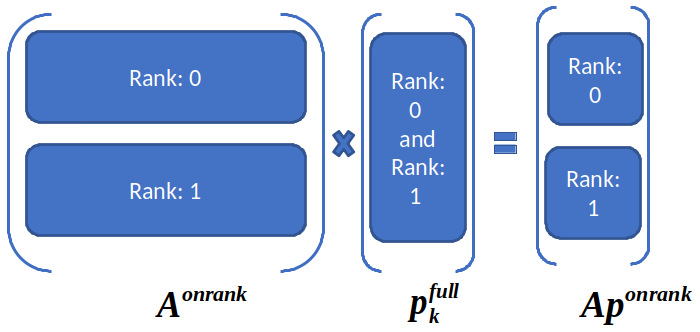
\includegraphics[width=0.45\textwidth]{plots/mpio_Ap.png}
	\end{center}
	\caption{Matrix-vector product on multiple ranks}
	\label{fig2} 
\end{figure}
The subsequent operations operations to get the new update vector $\mathbf{p_{k+1}}$ are done using the scaled vector addition and dot product kernels. The new update vector, however is stored partially on each rank based on the calculations from that rank.
\begin{figure}[H]
	\begin{center}
		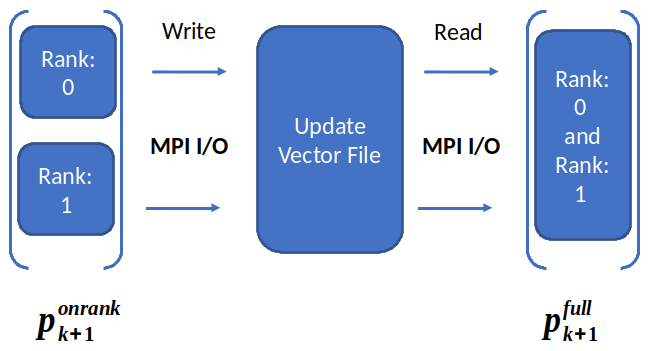
\includegraphics[width=0.45\textwidth]{plots/mpio_pupdate.png}
	\end{center}
	\caption{Partial update vector on each rank to full update vector using MPI I/O}
	\label{fig3} 
\end{figure}

\texttt{MPI\_File\_write\_at()} routine is used to write the partial update vector on each rank to a common file \texttt{update\_vector}. After all ranks finish writing the update vector to the file, using \texttt{MPI\_File\_read\_all()} the full update vector is read into a variable. Therefore, all ranks will have a copy of the full update vector for the matrix vector multiplication in the next iteration.

\subsubsection{Writing Final Result}
The solution to given linear system i.e. the result vector is also stored in each processor partially. The results were written to output file(s) in two ways -- 
\begin{enumerate}
	\item To one common result file using \texttt{MPI\_File\_write\_at()} ensuring each processor writes the partial result in the right location
	\item To multiple result files (one from each rank) using \texttt{MPI\_File\_write\_all()}
\end{enumerate}


\section{Performance Analysis}
The performance of parallel conjugate gradient solver is tested on \emph{AiMOS} for different systems with varying sizes. We tested two versions of the solver, the CPU only version and hybrid CPU/GPU version. Both strong and weak scaling analysis are conducted. These test results are discussed in this section. 
\subsection{Problem Definition}
Numerical analysis of steady 1D heat equation is considered for the performance analysis of the parallel conjugate gradient solver. Steady state heat equation in 1D is given as:
\begin{equation}\label{heat}
\kappa\frac{\partial^2 T}{\partial x^2}= f(x)
\end{equation}
Here, $T$ is the temperature, $\kappa$ is thermal conductivity and $f(x)$ is the source term. Numerical analysis of Eq. \eqref{heat} involves discretizing the domain into small segments and solving the equation using finite difference technique. This ultimately leads to solving a system of linear equations. The coefficient matrix obtained here is a sparse matrix with tri-diagonal banded structure. Bases on number of discretized segments, systems with varying sizes are obtained for performance analysis. 

\subsection{MPI Performance}\label{mpi_perfrom}
In this subsection performance analysis of MPI only version of the solver is discusses. Strong scaling study is conducted on 7 different systems of size $1K\times 1K$, $2.5K\times 2.5K$, $5K\times 5K$, $10K\times 10K$, $20K\times 20K$, $50K\times 50K$ and $100K\times 100K$. The number of MPI ranks is varied from 1-6 and 12. Plots for run-time analysis of strong scaling study are displayed in Fig. \ref{strong1}

\begin{figure*}
	\begin{subfigure}{0.4\textwidth}
		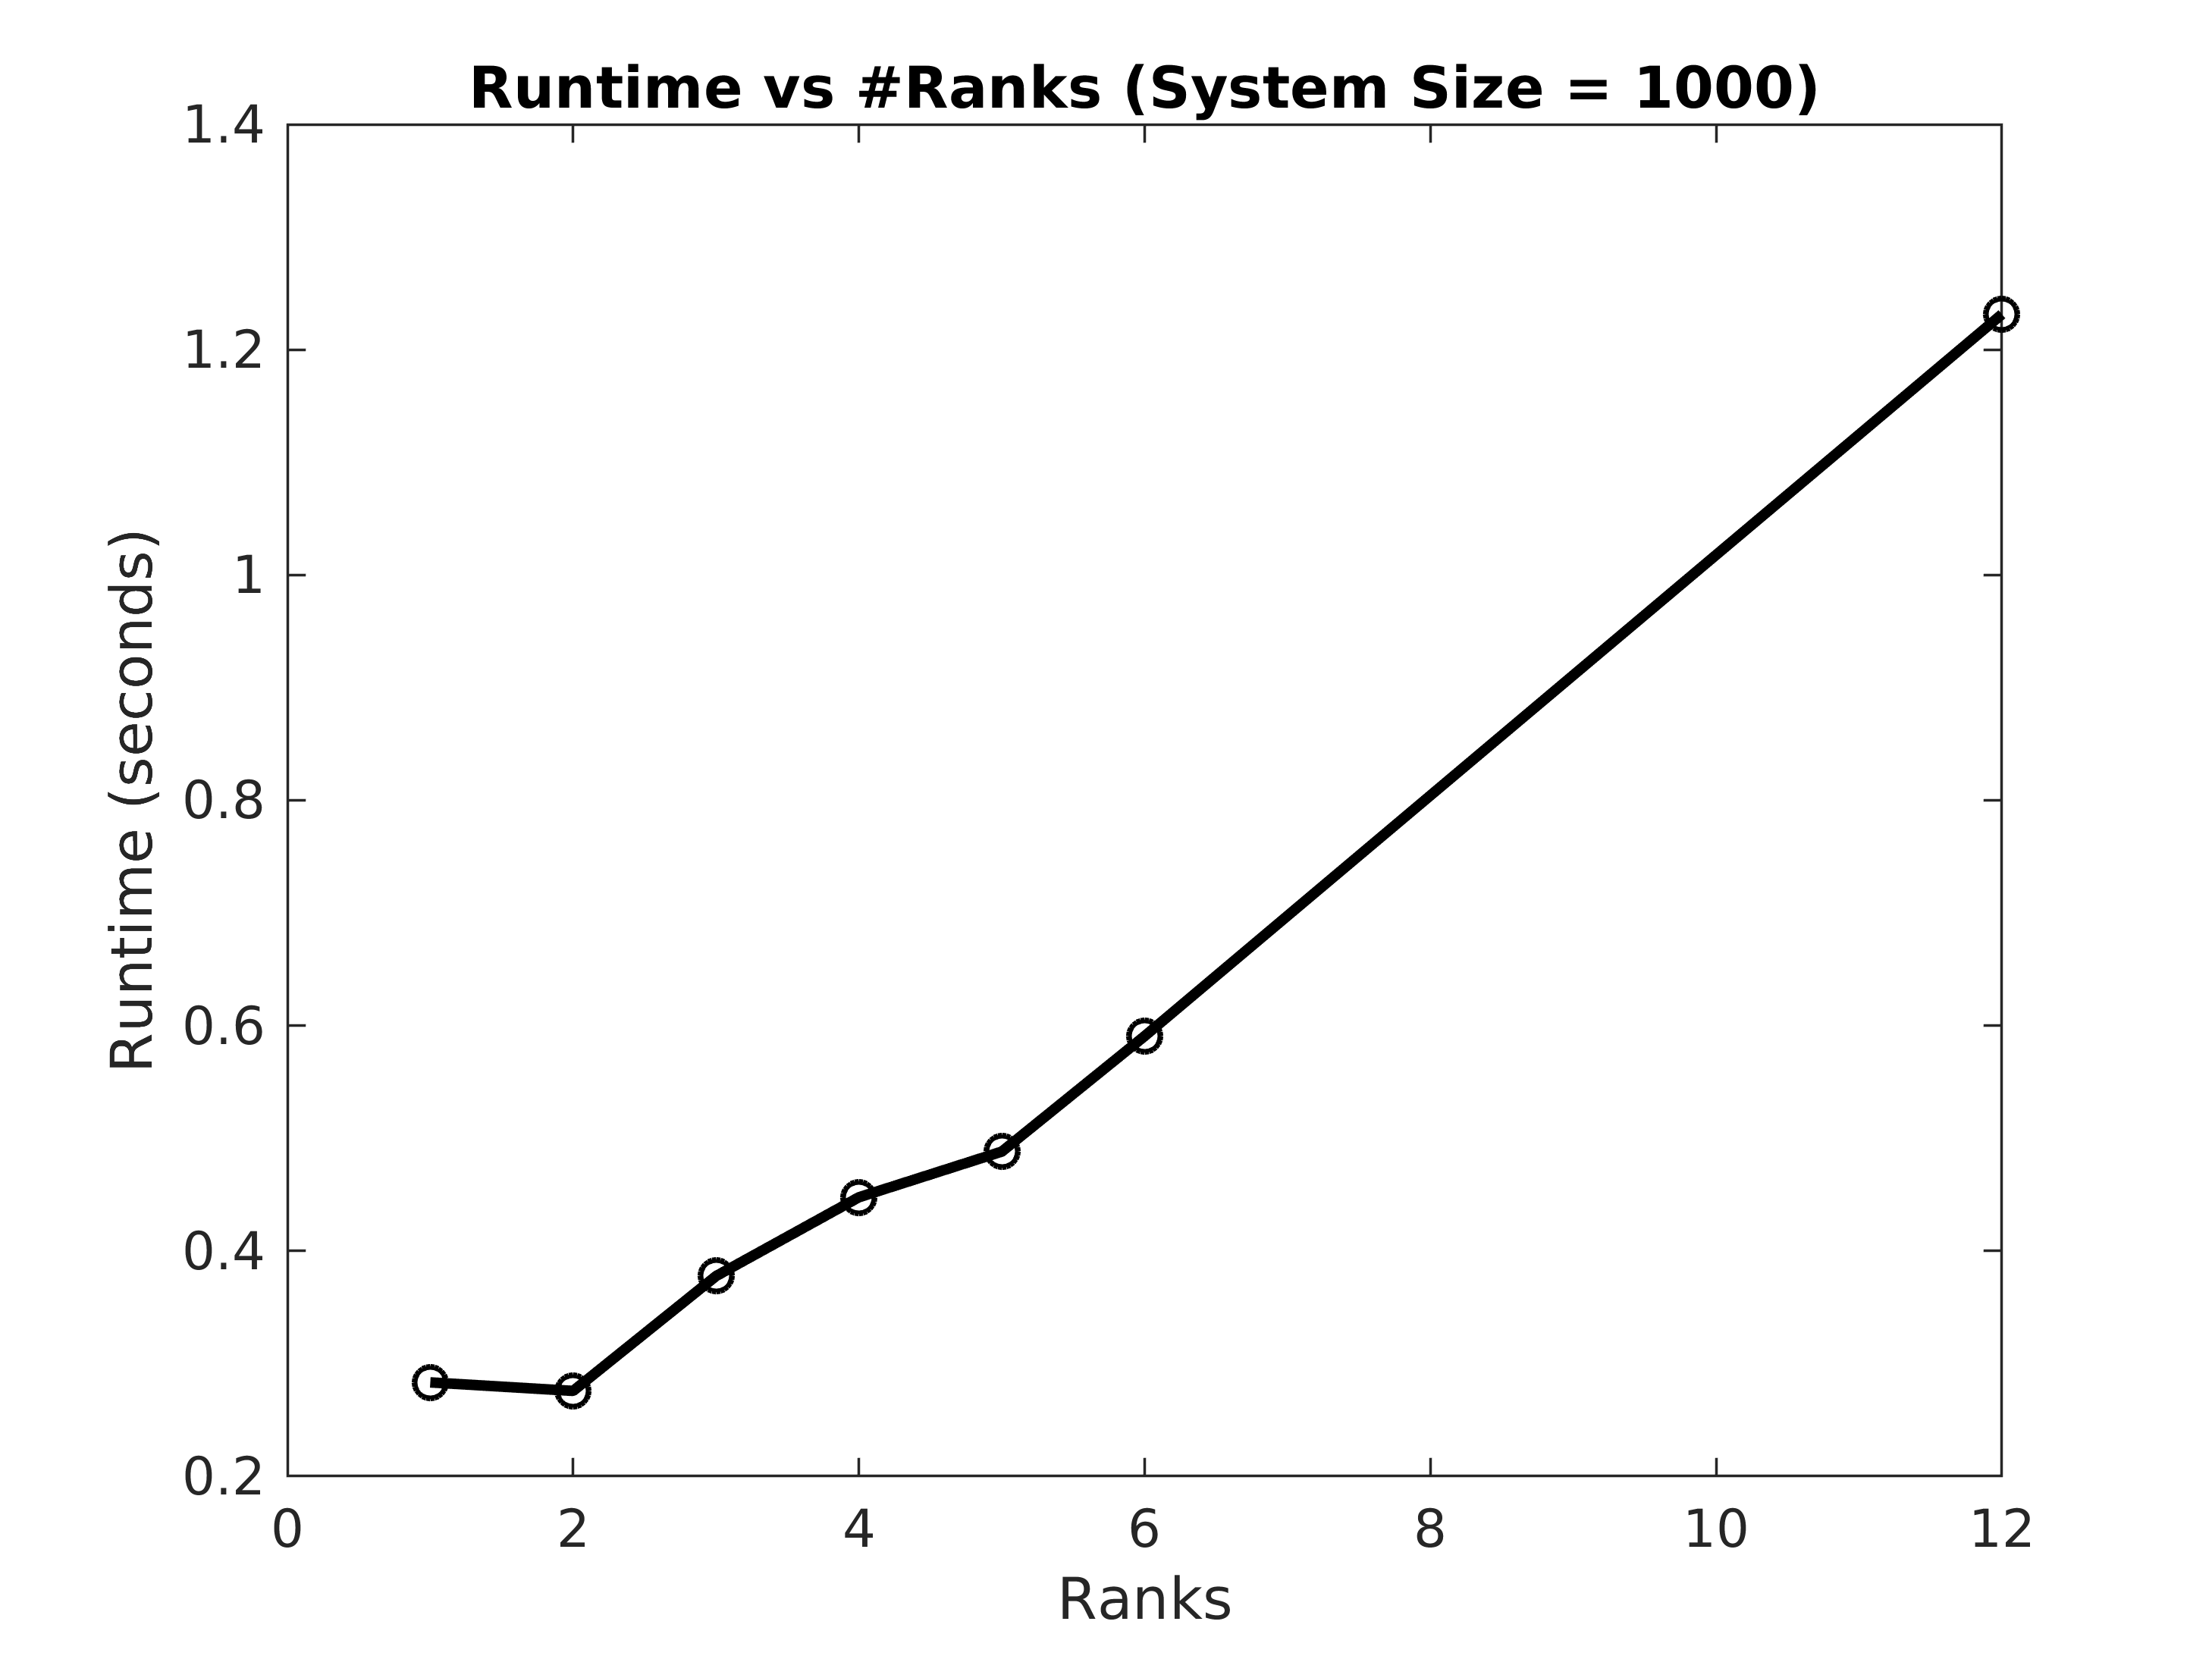
\includegraphics[trim= 20 5 35 10,clip, width=0.95\linewidth, height=5cm]{plots/MPI_strong_1k.png} 
		\caption{}
	\end{subfigure}
	\begin{subfigure}{0.4\textwidth}
		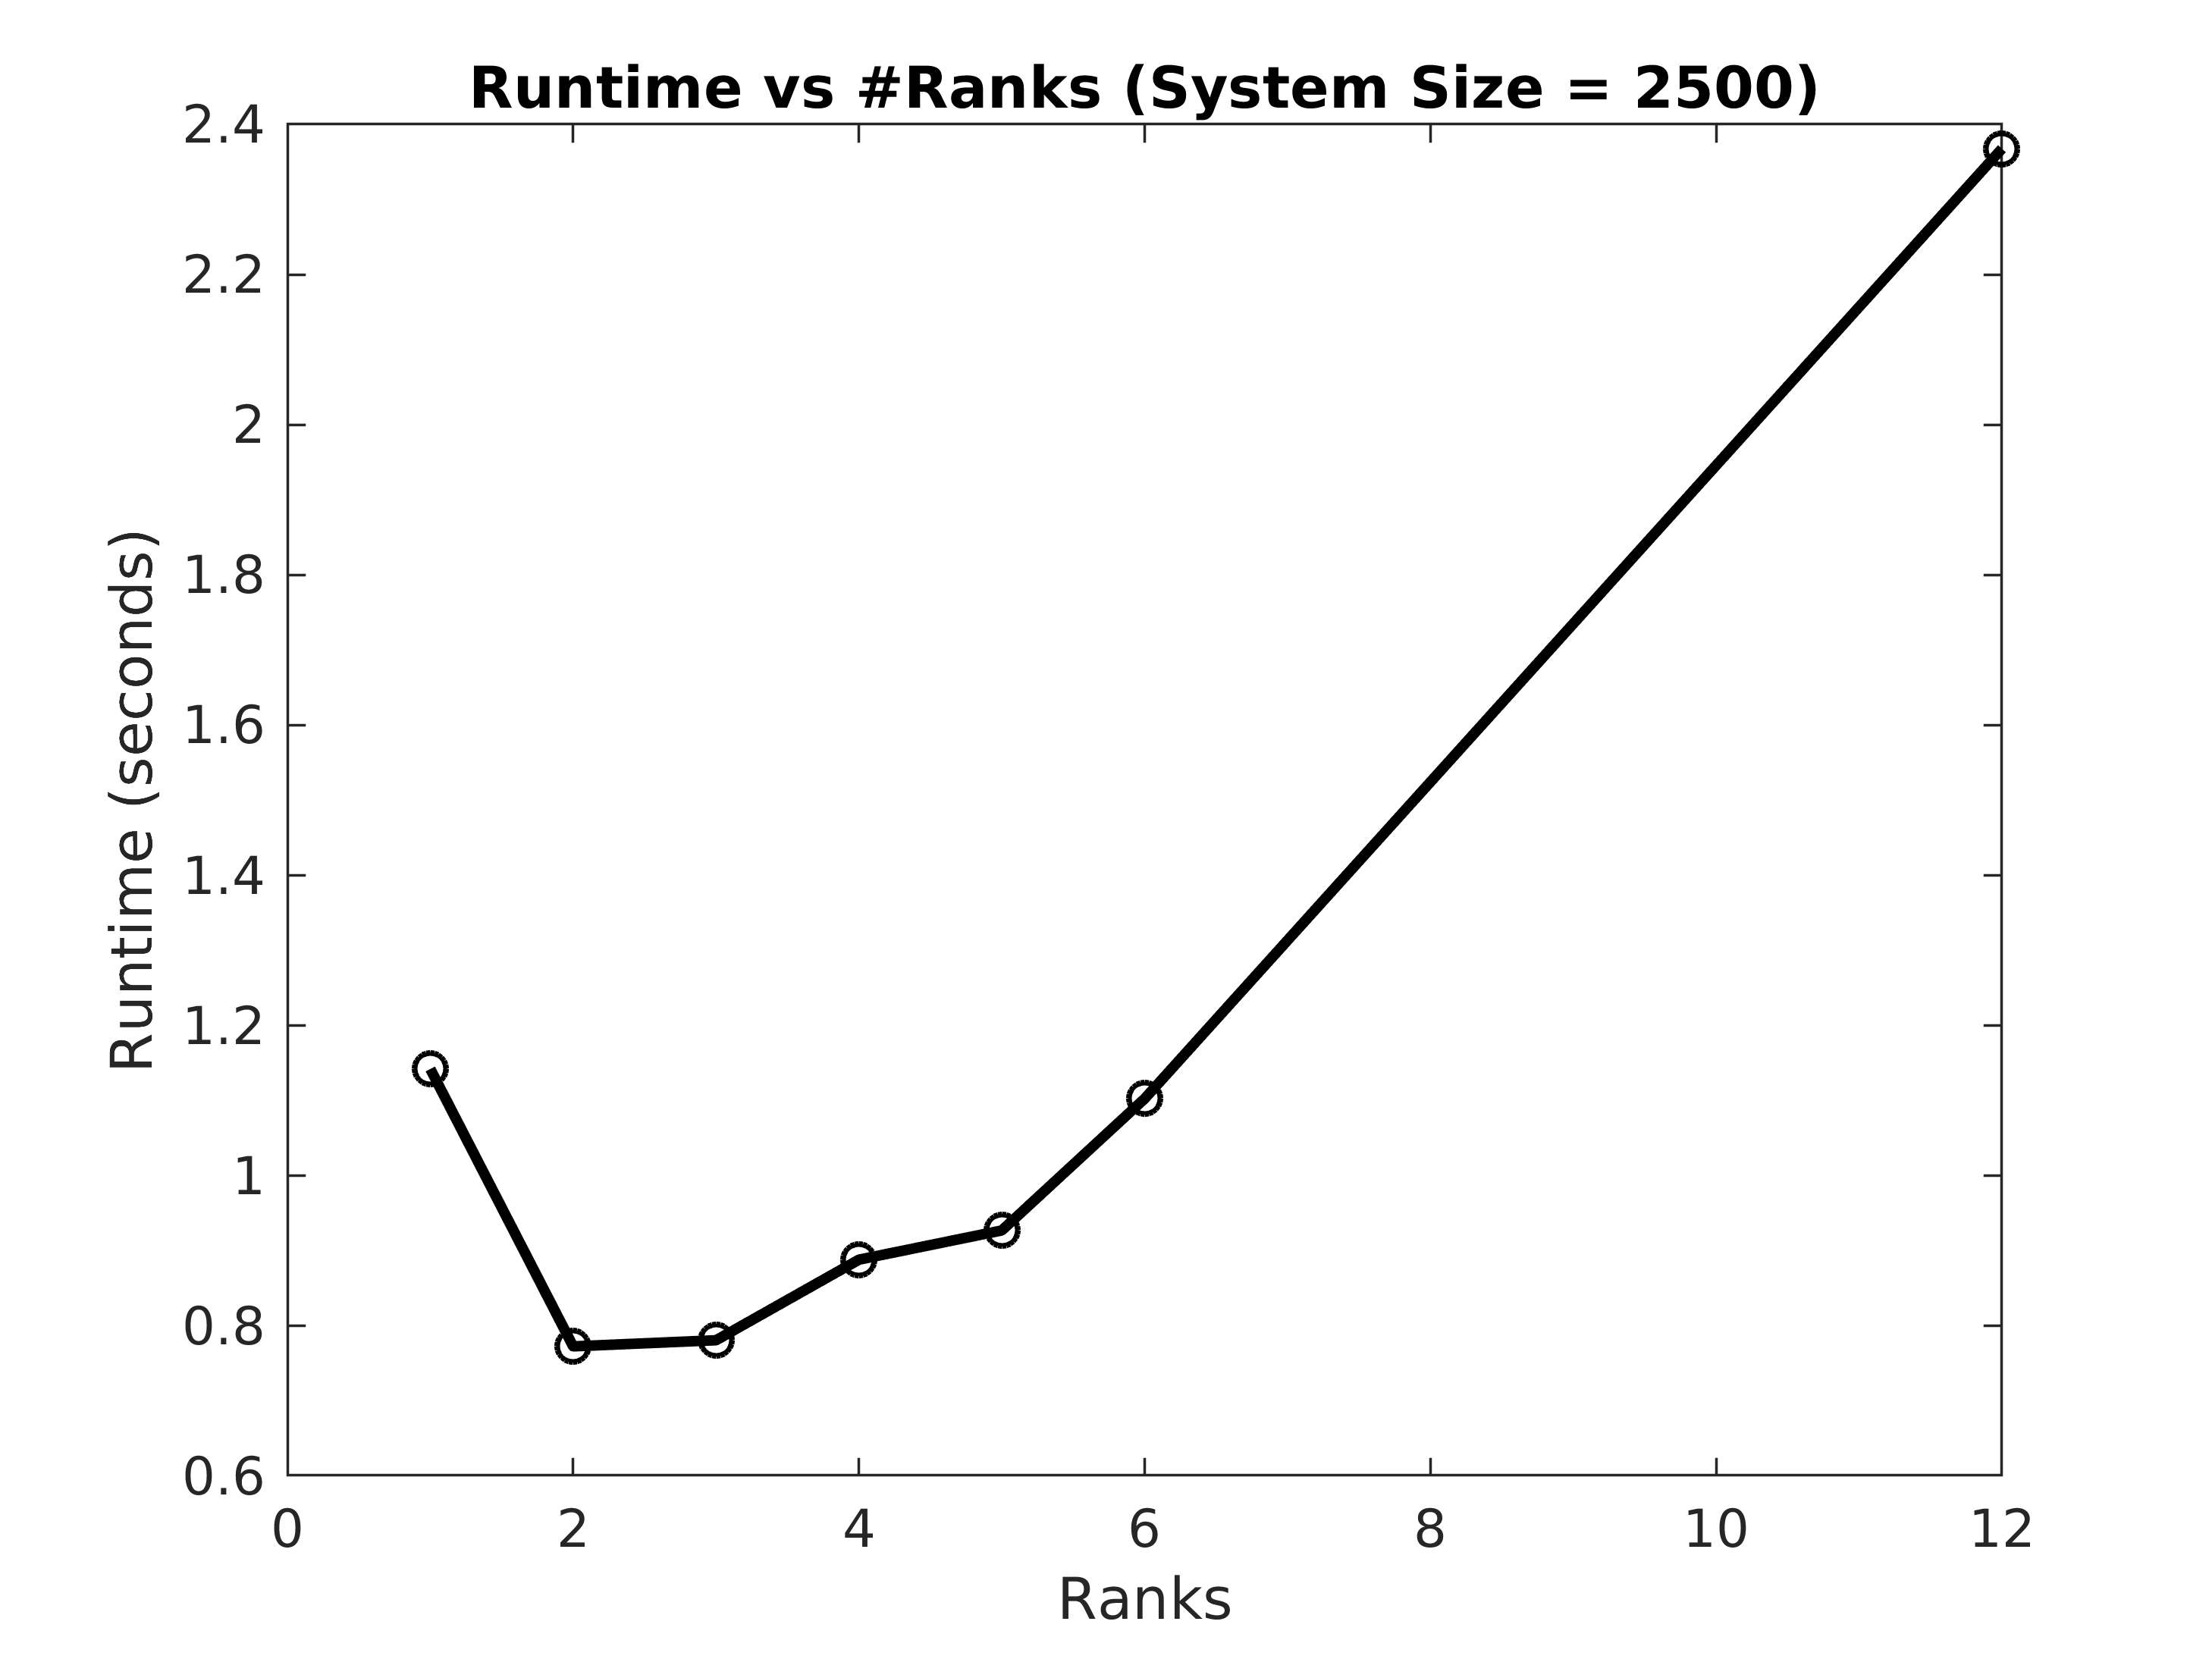
\includegraphics[trim= 20 5 35 10,clip, width=0.95\linewidth, height=5cm]{plots/MPI_strong_2k.png}
		\caption{}
	\end{subfigure}
	\begin{subfigure}{0.4\textwidth}
		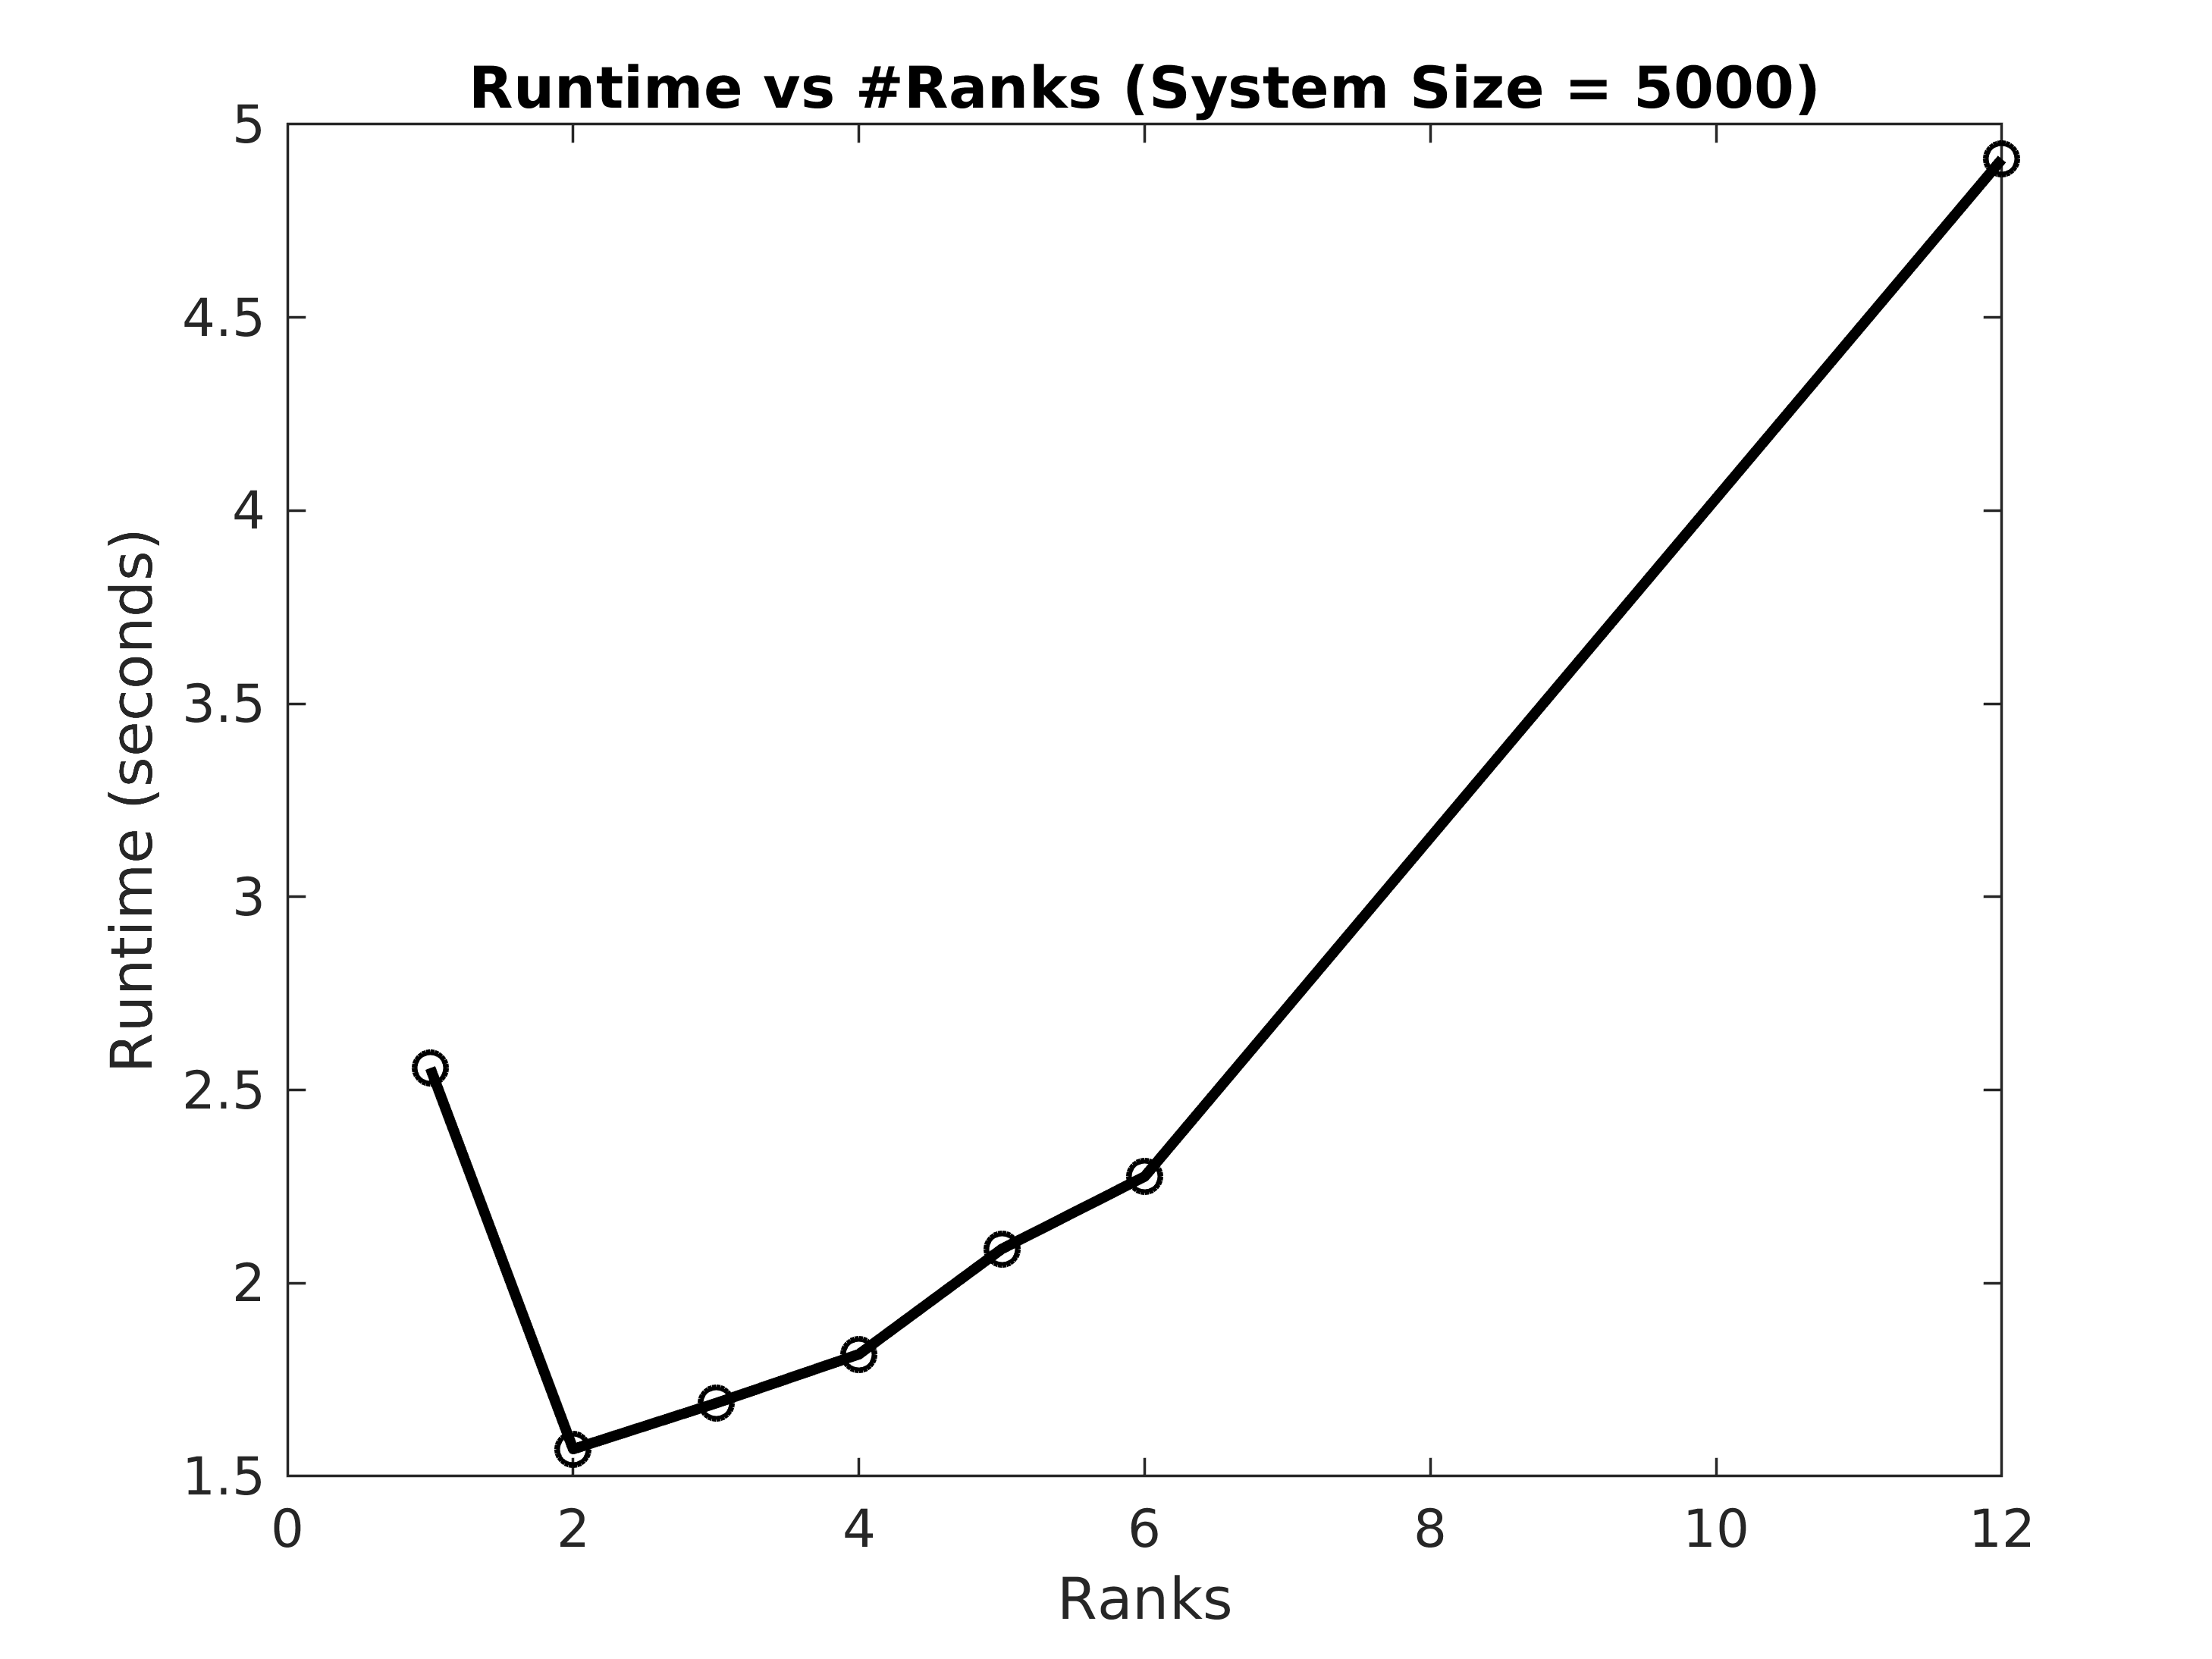
\includegraphics[trim= 20 5 35 10,clip, width=0.95\linewidth, height=5cm]{plots/MPI_strong_5k.png}
		\caption{}
	\end{subfigure}
	\begin{subfigure}{0.4\textwidth}
		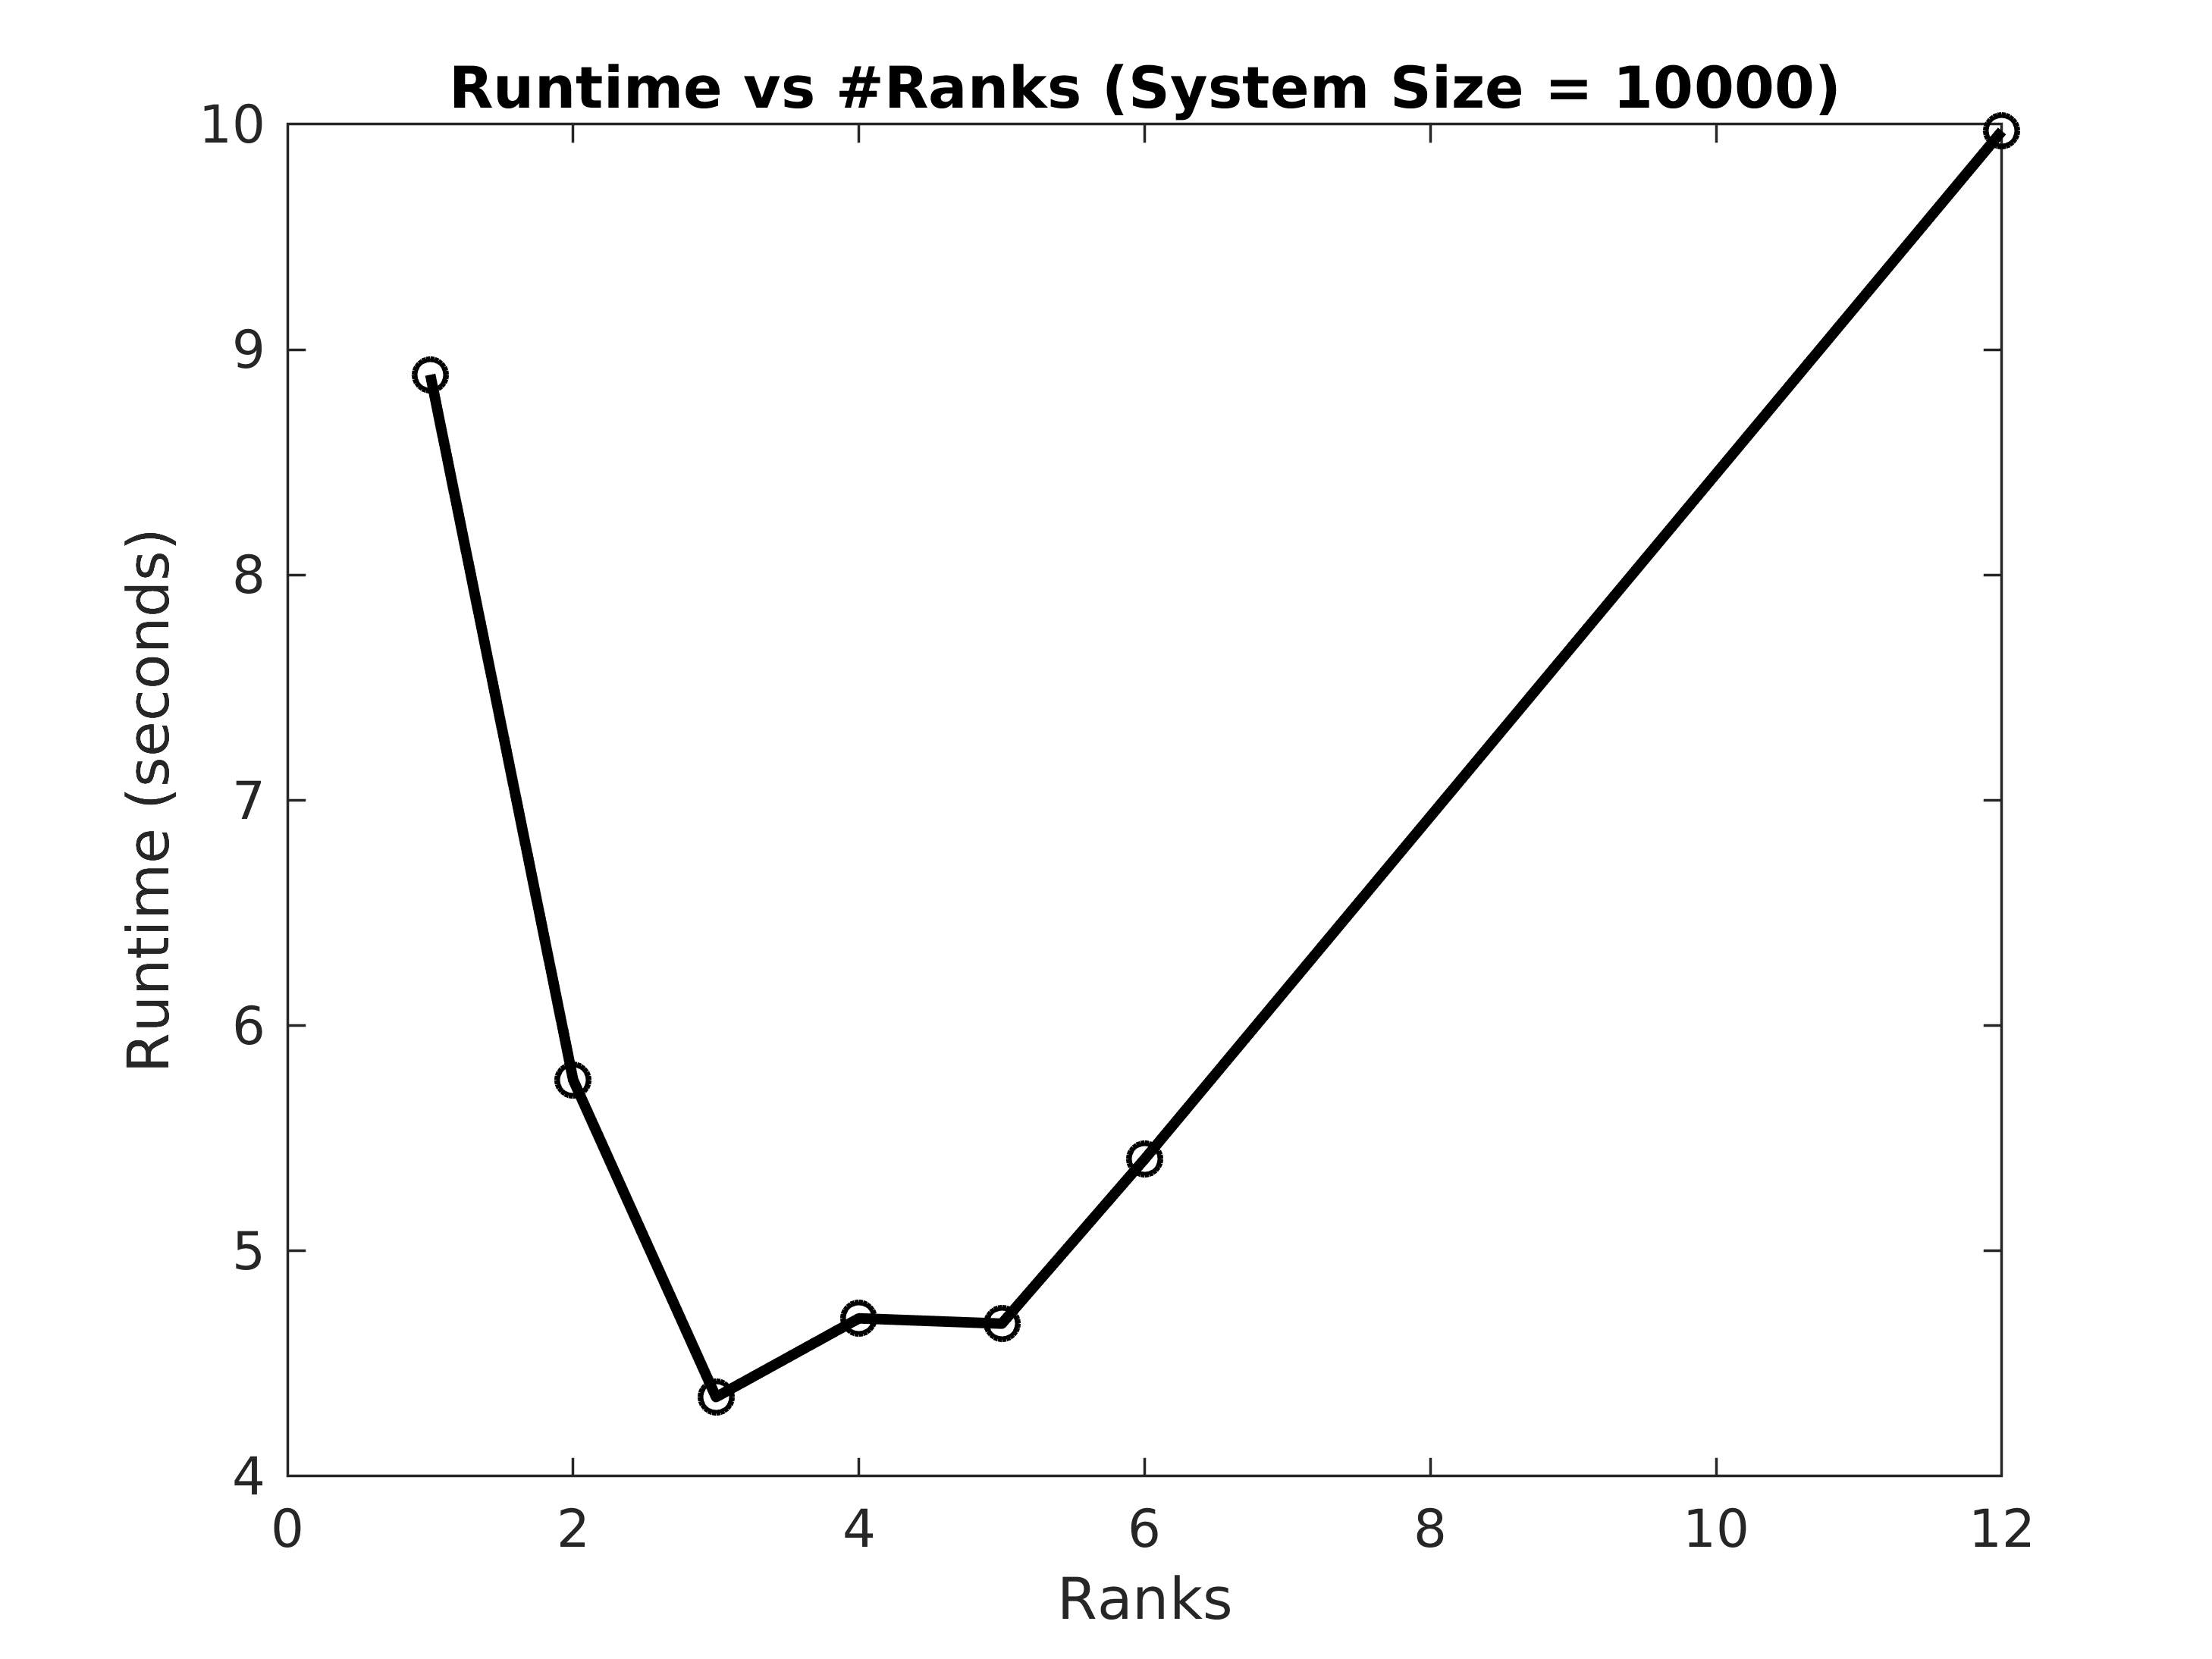
\includegraphics[trim= 20 5 35 10,clip, width=0.95\linewidth, height=5cm]{plots/MPI_strong_10k.png}
		\caption{}
	\end{subfigure}
	\begin{subfigure}{0.4\textwidth}
		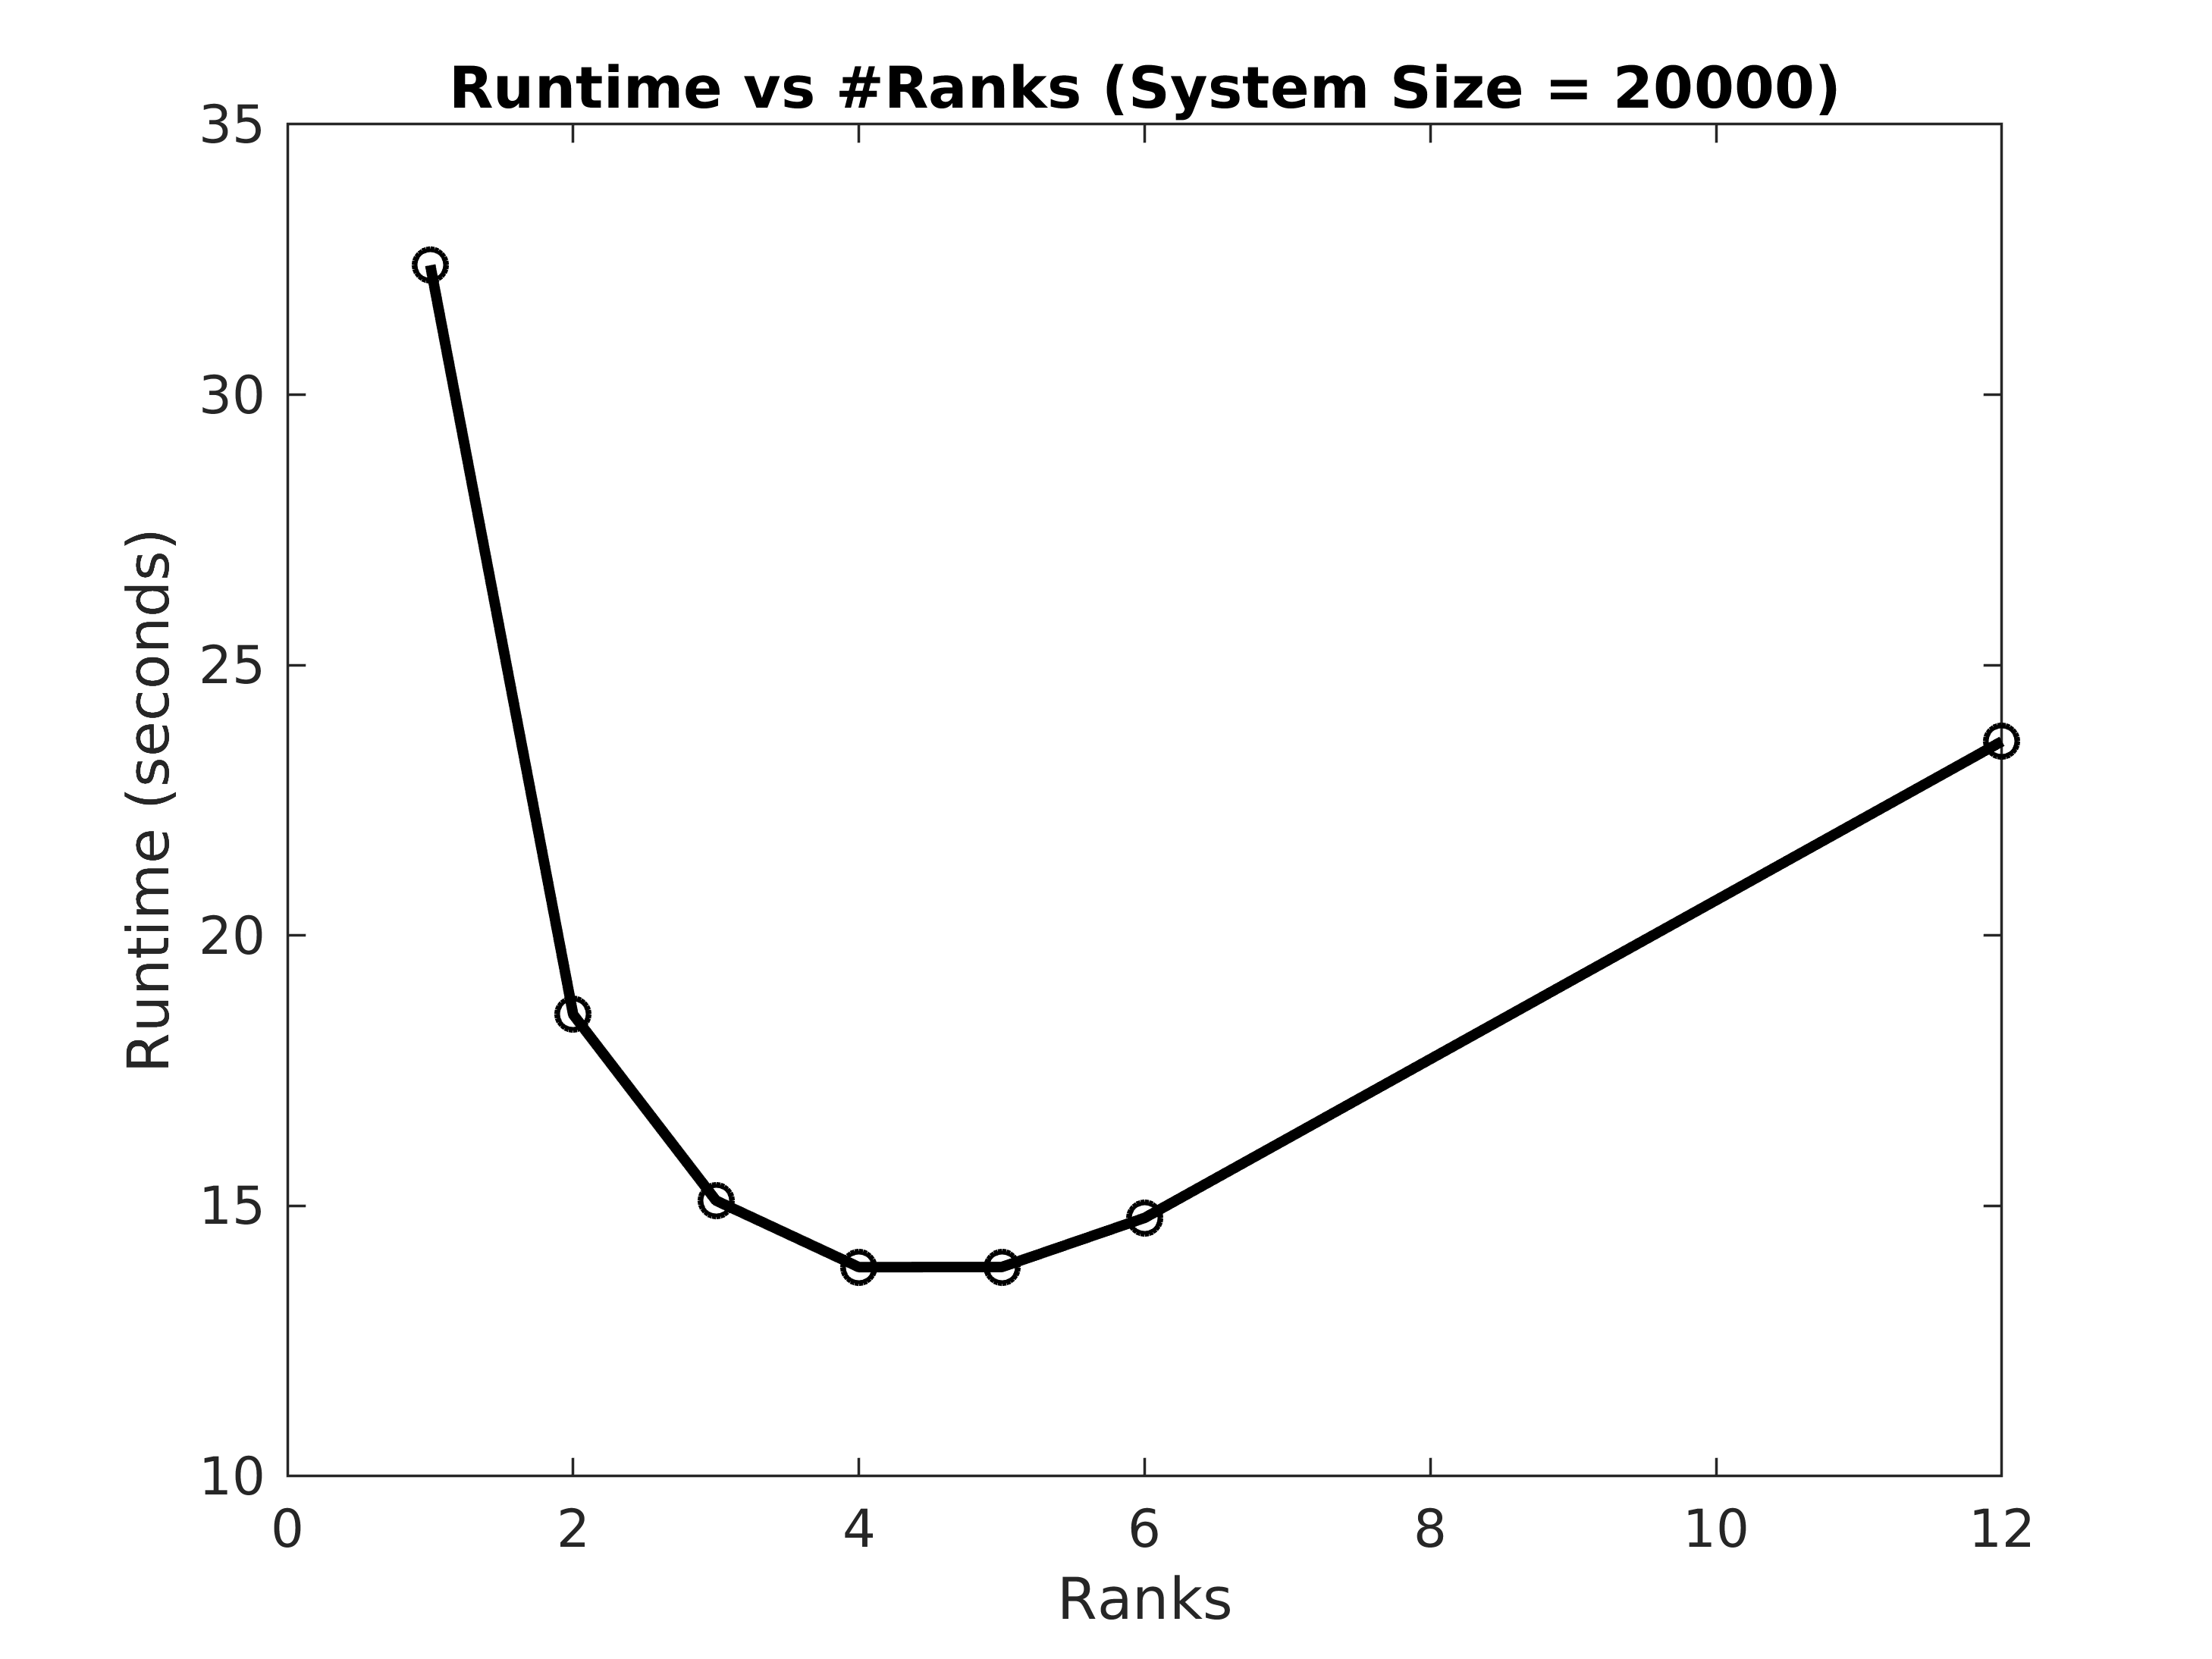
\includegraphics[trim= 20 5 35 10,clip, width=0.95\linewidth, height=5cm]{plots/MPI_strong_20k.png} 
		\caption{}
	\end{subfigure}
	\begin{subfigure}{0.4\textwidth}
		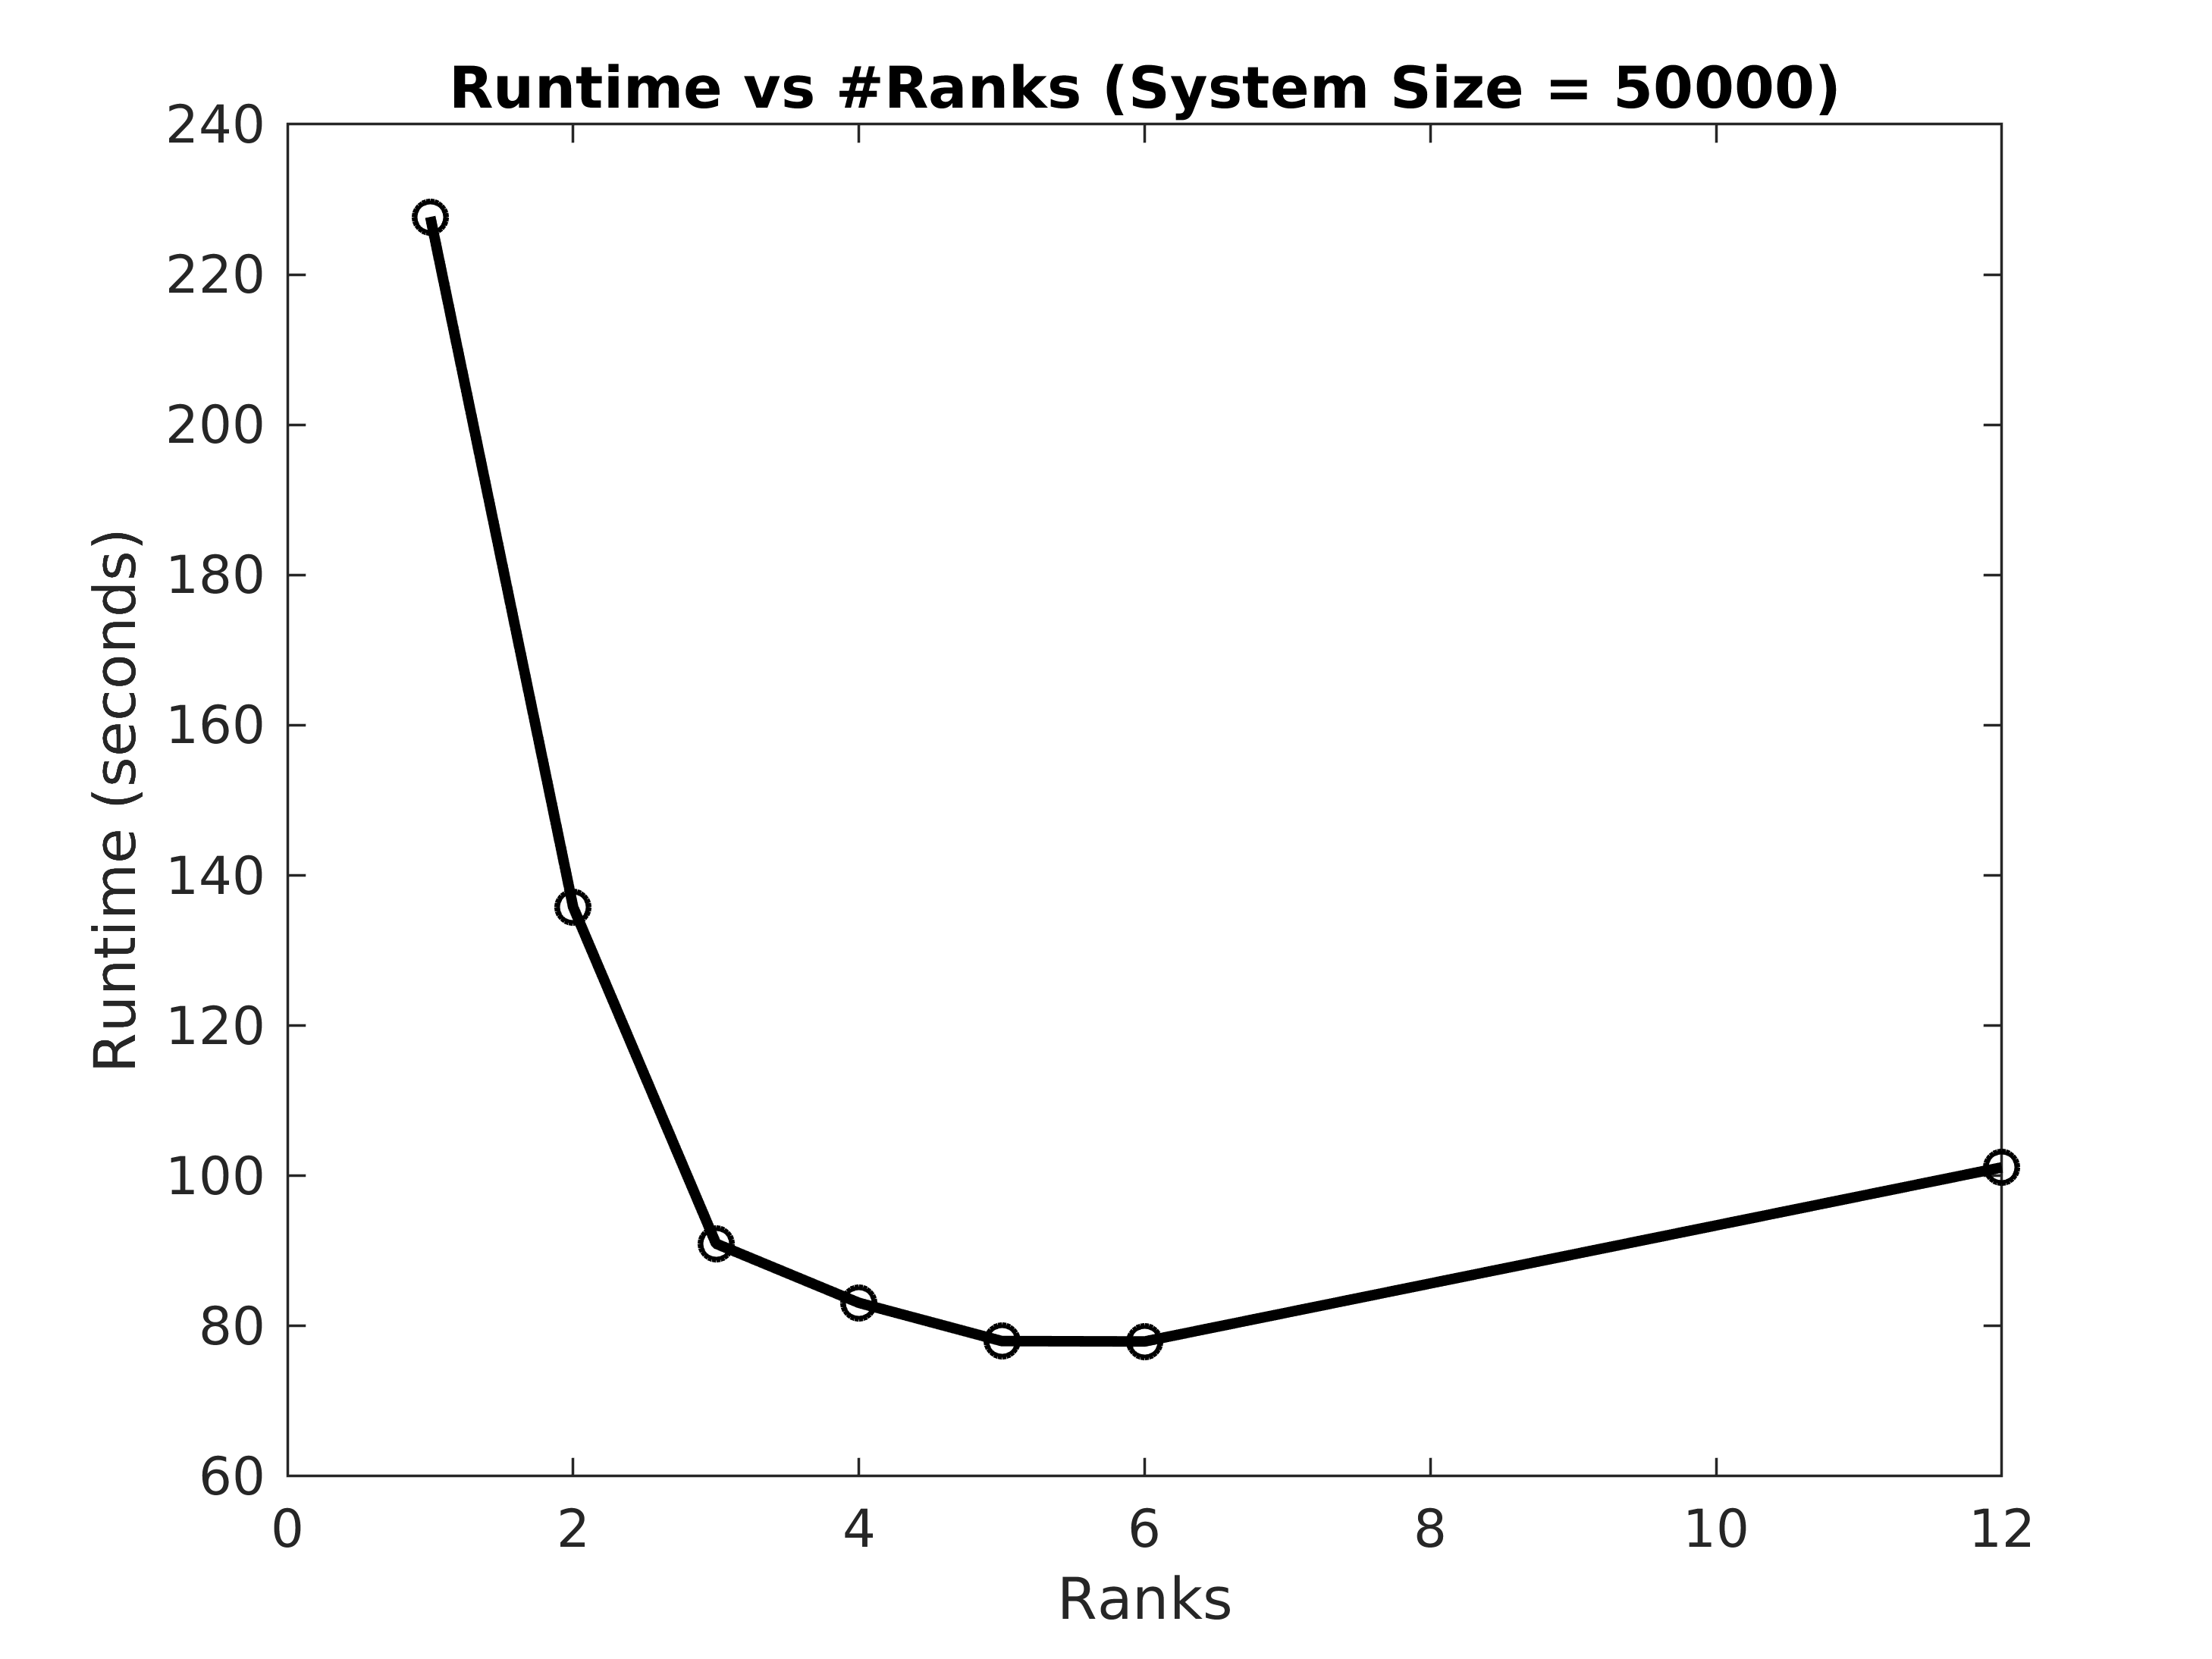
\includegraphics[trim= 20 5 35 10,clip, width=0.95\linewidth, height=5cm]{plots/MPI_strong_50k.png}
		\caption{}
	\end{subfigure}
	\begin{subfigure}{0.4\textwidth}
		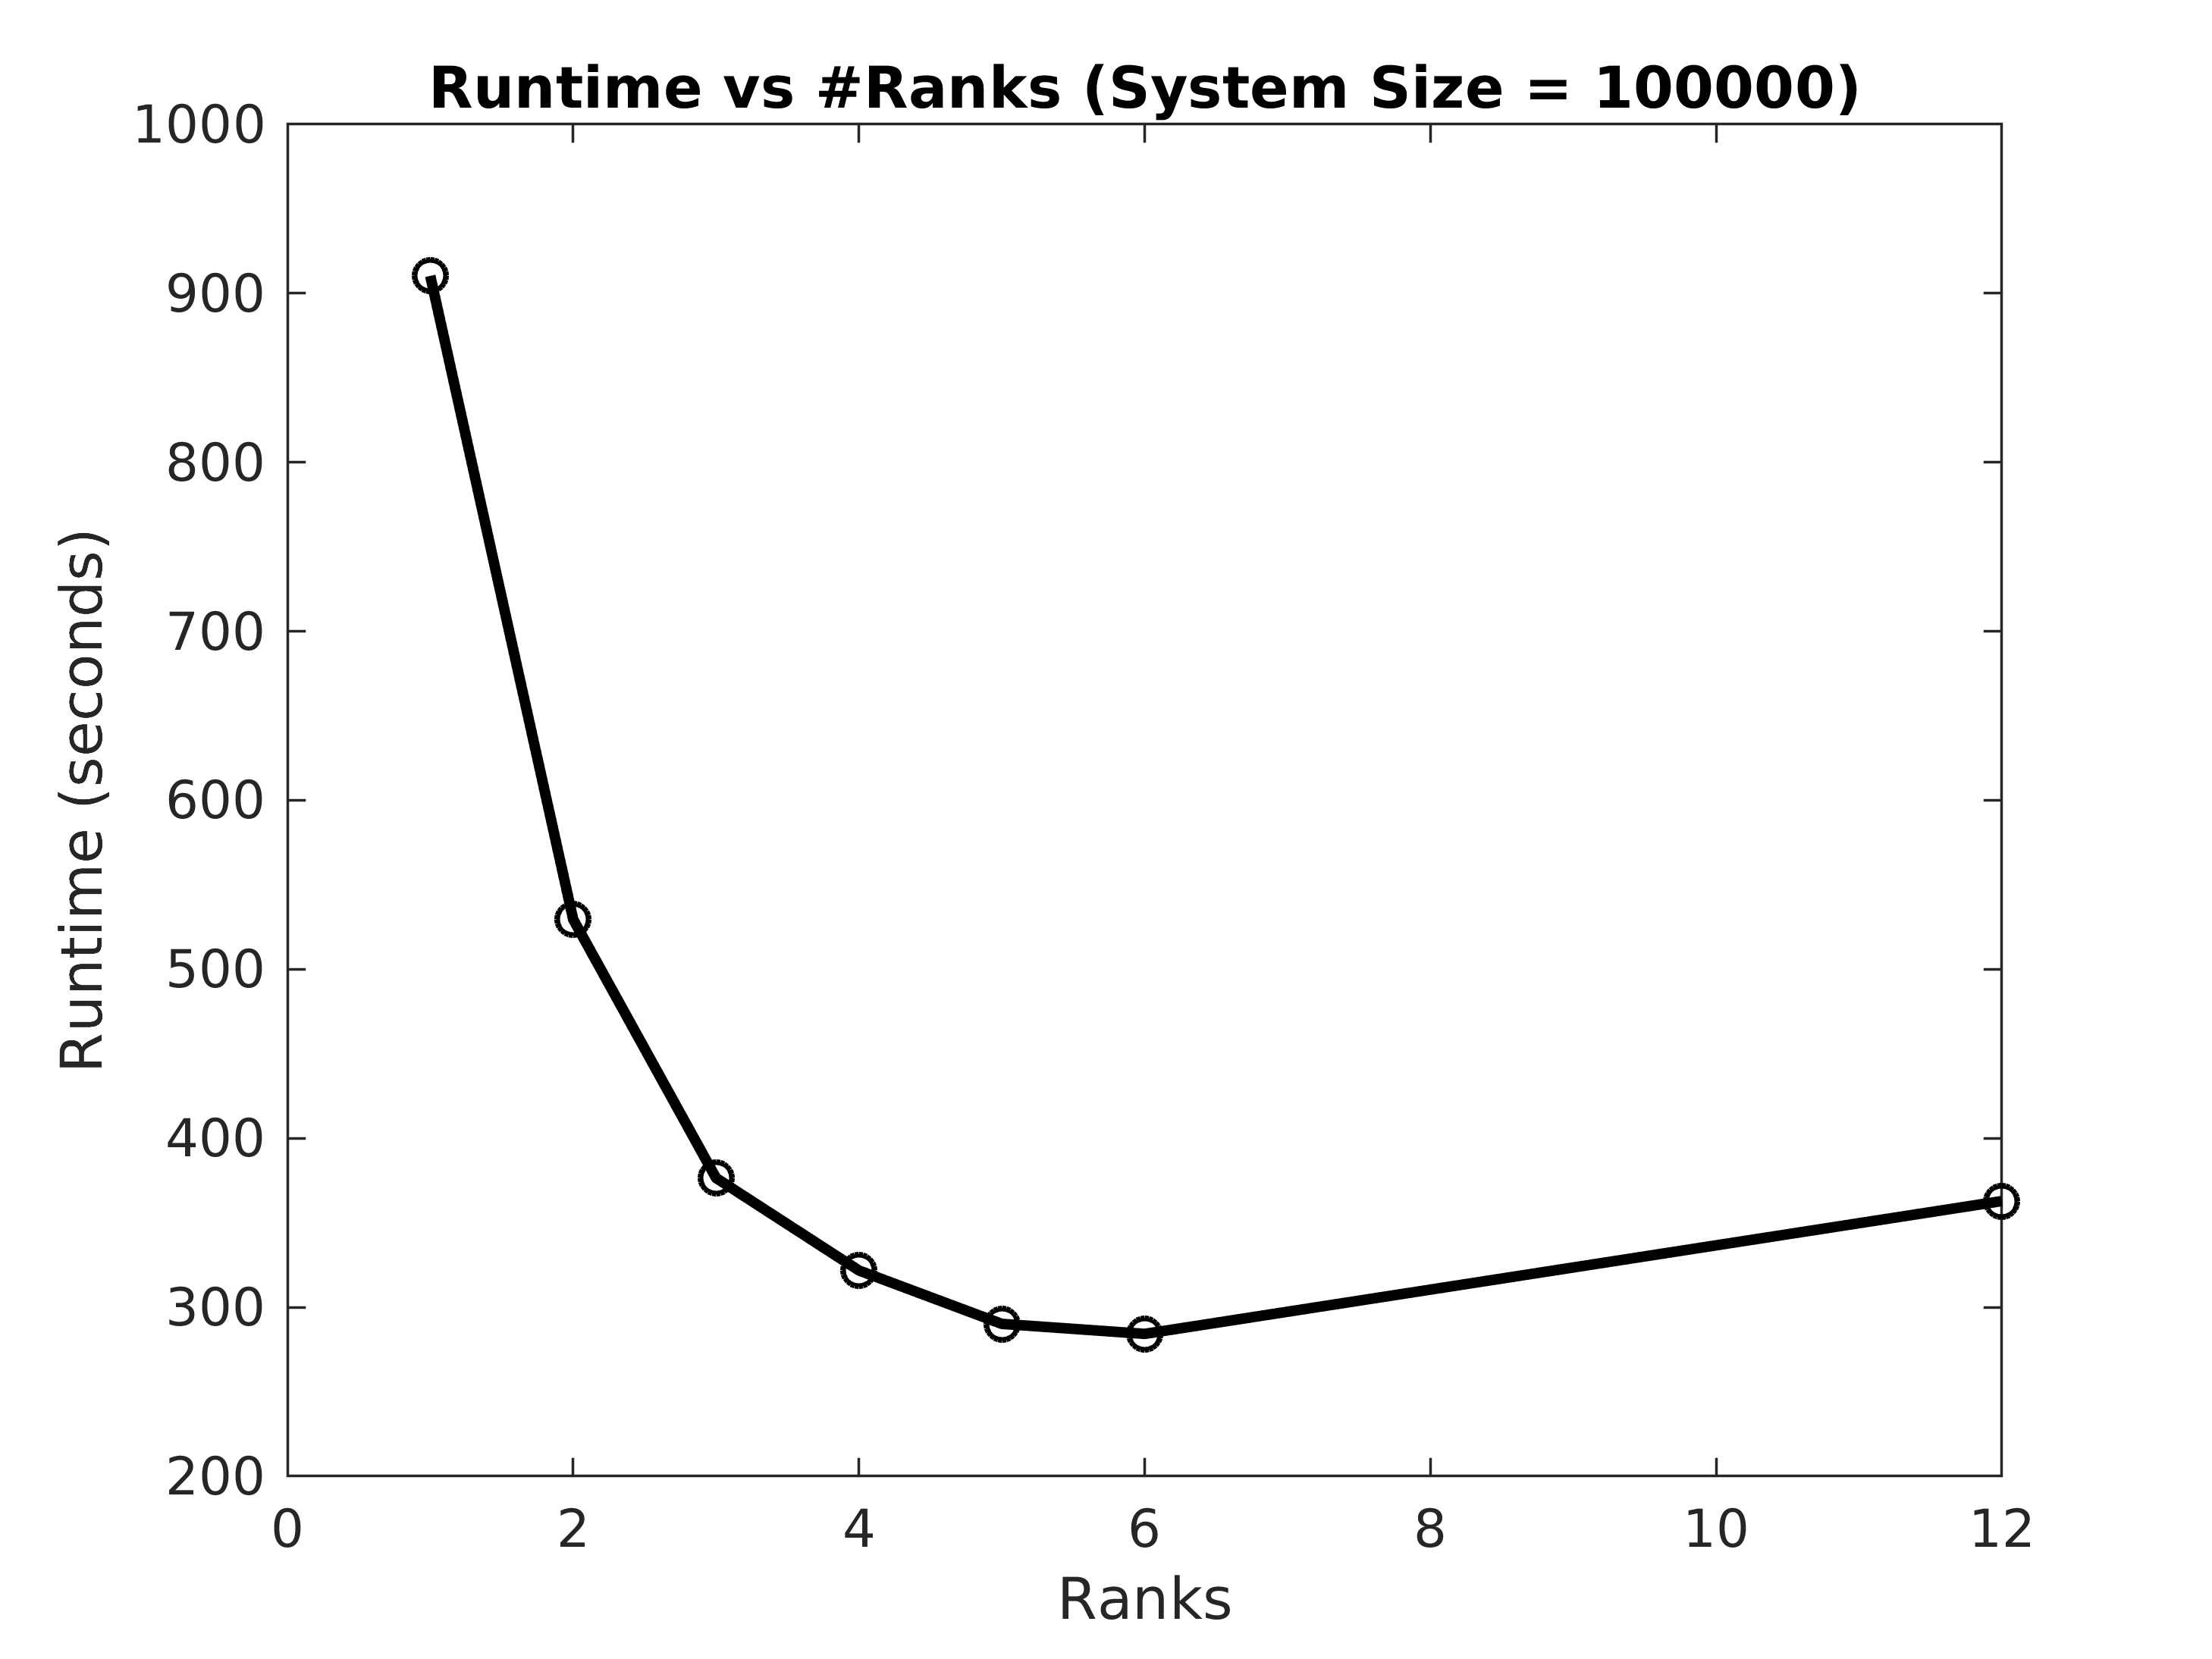
\includegraphics[trim= 20 5 35 10,clip, width=0.95\linewidth, height=5cm]{plots/MPI_strong_100k.png}
		\caption{}
	\end{subfigure}
	\caption{MPI only strong scaling analysis.}
	\label{strong1}
\end{figure*}

\begin{figure}[h!]
	\begin{center}
		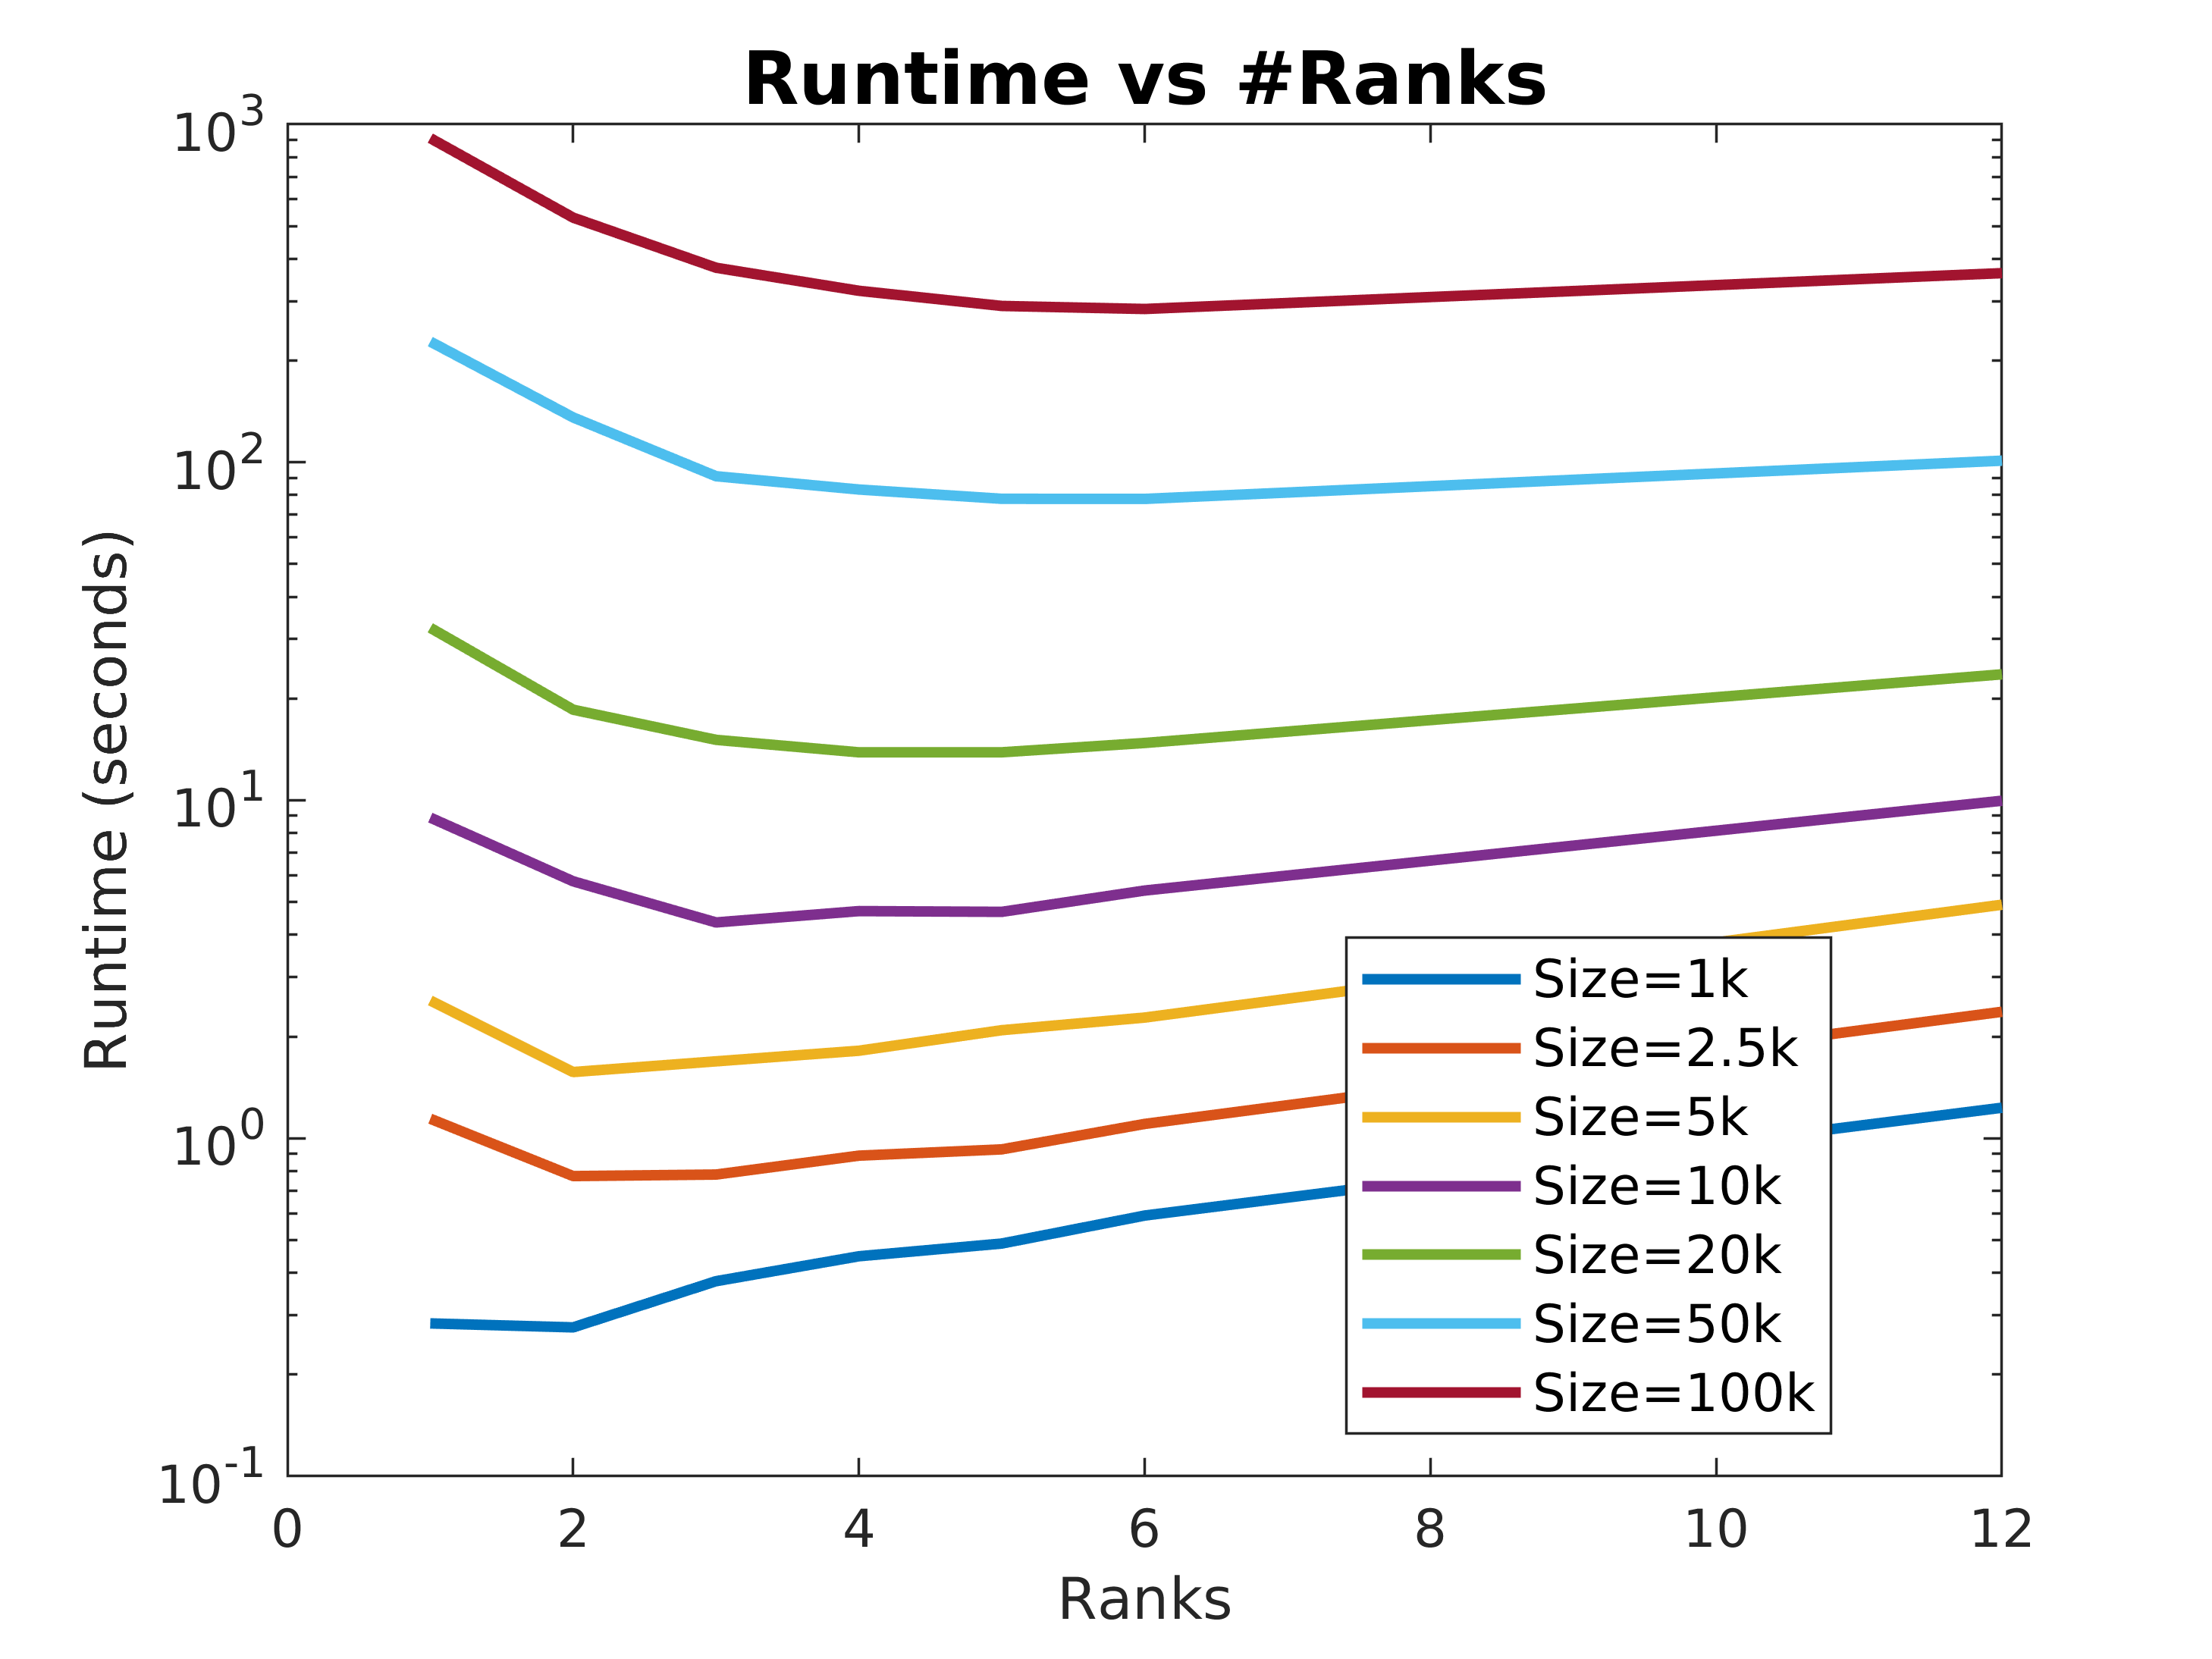
\includegraphics[width=0.35\textwidth]{plots/MPI_strong_allranks_log.png}
	\end{center}
	\caption{Run-time vs. no. of ranks for all cases}
	\label{strong2}      
\end{figure}

In Fig. \ref{strong2}, run-time analysis for all the cases is displayed. It can be observed that for size $1K\times 1K$, $2.5K\time 2.5K$ and $5K\times 5K$, there is a nominal speedup by using 2 ranks. But as we increase the ranks from 2 the run-time is increasing. For the larger systems we can observe the speedup with increase in number of ranks from 1-6. But for 12 ranks all the systems show different degrees of slowdown. 

To get better understanding of these results, we did performance analysis of the solver using an application \emph{GProf}. The results for system of size $50K\times 50K$ are shown in Table \ref{tab:gprof1}, \ref{tab:gprof2}, \ref{tab:gprof3}. The operations which take maximum time are matrix-vector multiplication, vector-vector addition and vector-vector dot product. As we increase the ranks from 1-2 and eventually to 12, the speedup in all three operations can be observed. But all the ranks need synchronization before moving to the next iteration. If each rank handles relatively small number of rows, the idle time will increase because of synchronization. Hence using more than 2 ranks in only justified for large systems. 

\begin{table}[H]
	\scriptsize
	\caption{Profiling for 50k system size with 1 rank}
	\label{tab:gprof1}
	\begin{tabular}{|l|l|l|l|l|}
		\hline
		\multicolumn{1}{|l|}{\begin{tabular}[c]{@{}l@{}}\%\\ time\end{tabular}} & \multicolumn{1}{l|}{\begin{tabular}[c]{@{}l@{}}Cumulative\\ seconds\end{tabular}} & \multicolumn{1}{l|}{\begin{tabular}[c]{@{}l@{}}self\\ seconds\end{tabular}} & \multicolumn{1}{l|}{\begin{tabular}[c]{@{}l@{}}self\\ calls\end{tabular}} & \multicolumn{1}{l|}{Function}    \\ \hline
		44.68                                                                   & 92.54                                                                             & 92.54                                                                       & 50010                                                                     & matrix\_vector\_product\_onrank  \\
		27.54                                                                   & 149.58                                                                            & 57.04                                                                       & 150027                                                                    & vector\_scaled\_addition\_onrank \\
		26.80                                                                   & 205.08                                                                            & 55.50                                                                       & 150027                                                                    & vector\_dot\_product\_onrank \\ \hline   
	\end{tabular}
\end{table}

\begin{table}[H]
	\scriptsize
	\caption{Profiling for 50k system size with 2 ranks}
	\label{tab:gprof2}
	\begin{tabular}{|l|l|l|l|l|}
		\hline
		\multicolumn{1}{|l|}{\begin{tabular}[c]{@{}l@{}}\%\\ time\end{tabular}} & \multicolumn{1}{l|}{\begin{tabular}[c]{@{}l@{}}Cumulative\\ seconds\end{tabular}} & \multicolumn{1}{l|}{\begin{tabular}[c]{@{}l@{}}self\\ seconds\end{tabular}} & \multicolumn{1}{l|}{\begin{tabular}[c]{@{}l@{}}self\\ calls\end{tabular}} & \multicolumn{1}{l|}{Function}    \\ \hline
		47.01                                                                   & 48.63                                                                             & 48.63                                                                       & 50009                                                                     & matrix\_vector\_product\_onrank  \\
		26.44                                                                   & 75.98                                                                            & 27.35                                                                       & 150024                                                                    & vector\_scaled\_addition\_onrank \\
		25.76                                                                   & 102.63                                                                            & 26.65                                                                       & 150024                                                                    & vector\_dot\_product\_onrank \\ \hline   
	\end{tabular}
\end{table}

\begin{table}[H]
	\scriptsize
	\caption{Profiling for 50k system size with 12 ranks}
	\label{tab:gprof3}
	\begin{tabular}{|l|l|l|l|l|}
		\hline
		\multicolumn{1}{|l|}{\begin{tabular}[c]{@{}l@{}}\%\\ time\end{tabular}} & \multicolumn{1}{l|}{\begin{tabular}[c]{@{}l@{}}Cumulative\\ seconds\end{tabular}} & \multicolumn{1}{l|}{\begin{tabular}[c]{@{}l@{}}self\\ seconds\end{tabular}} & \multicolumn{1}{l|}{\begin{tabular}[c]{@{}l@{}}self\\ calls\end{tabular}} & \multicolumn{1}{l|}{Function}    \\ \hline
		42.51                                                                   & 7.36                                                                             & 7.36                                                                       & 50006                                                                     & matrix\_vector\_product\_onrank  \\
		30.63                                                                   & 12.67                                                                            & 5.30                                                                       & 150015                                                                    & vector\_scaled\_addition\_onrank \\
		25.80                                                                   & 17.14                                                                            & 4.47                                                                       & 150015                                                                    & vector\_dot\_product\_onrank \\ \hline   
	\end{tabular}
\end{table}

The weak scaling study analyzes speedup with number of processors for fixed problem size per processor. This type of study is not possible on our solver as it would lead to an invalid system of equation. Run-time analysis vs. size of the problem for different number of ranks is displayed in Fig. \ref{weak}.

\begin{figure}
	\begin{subfigure}{0.3\textwidth}
		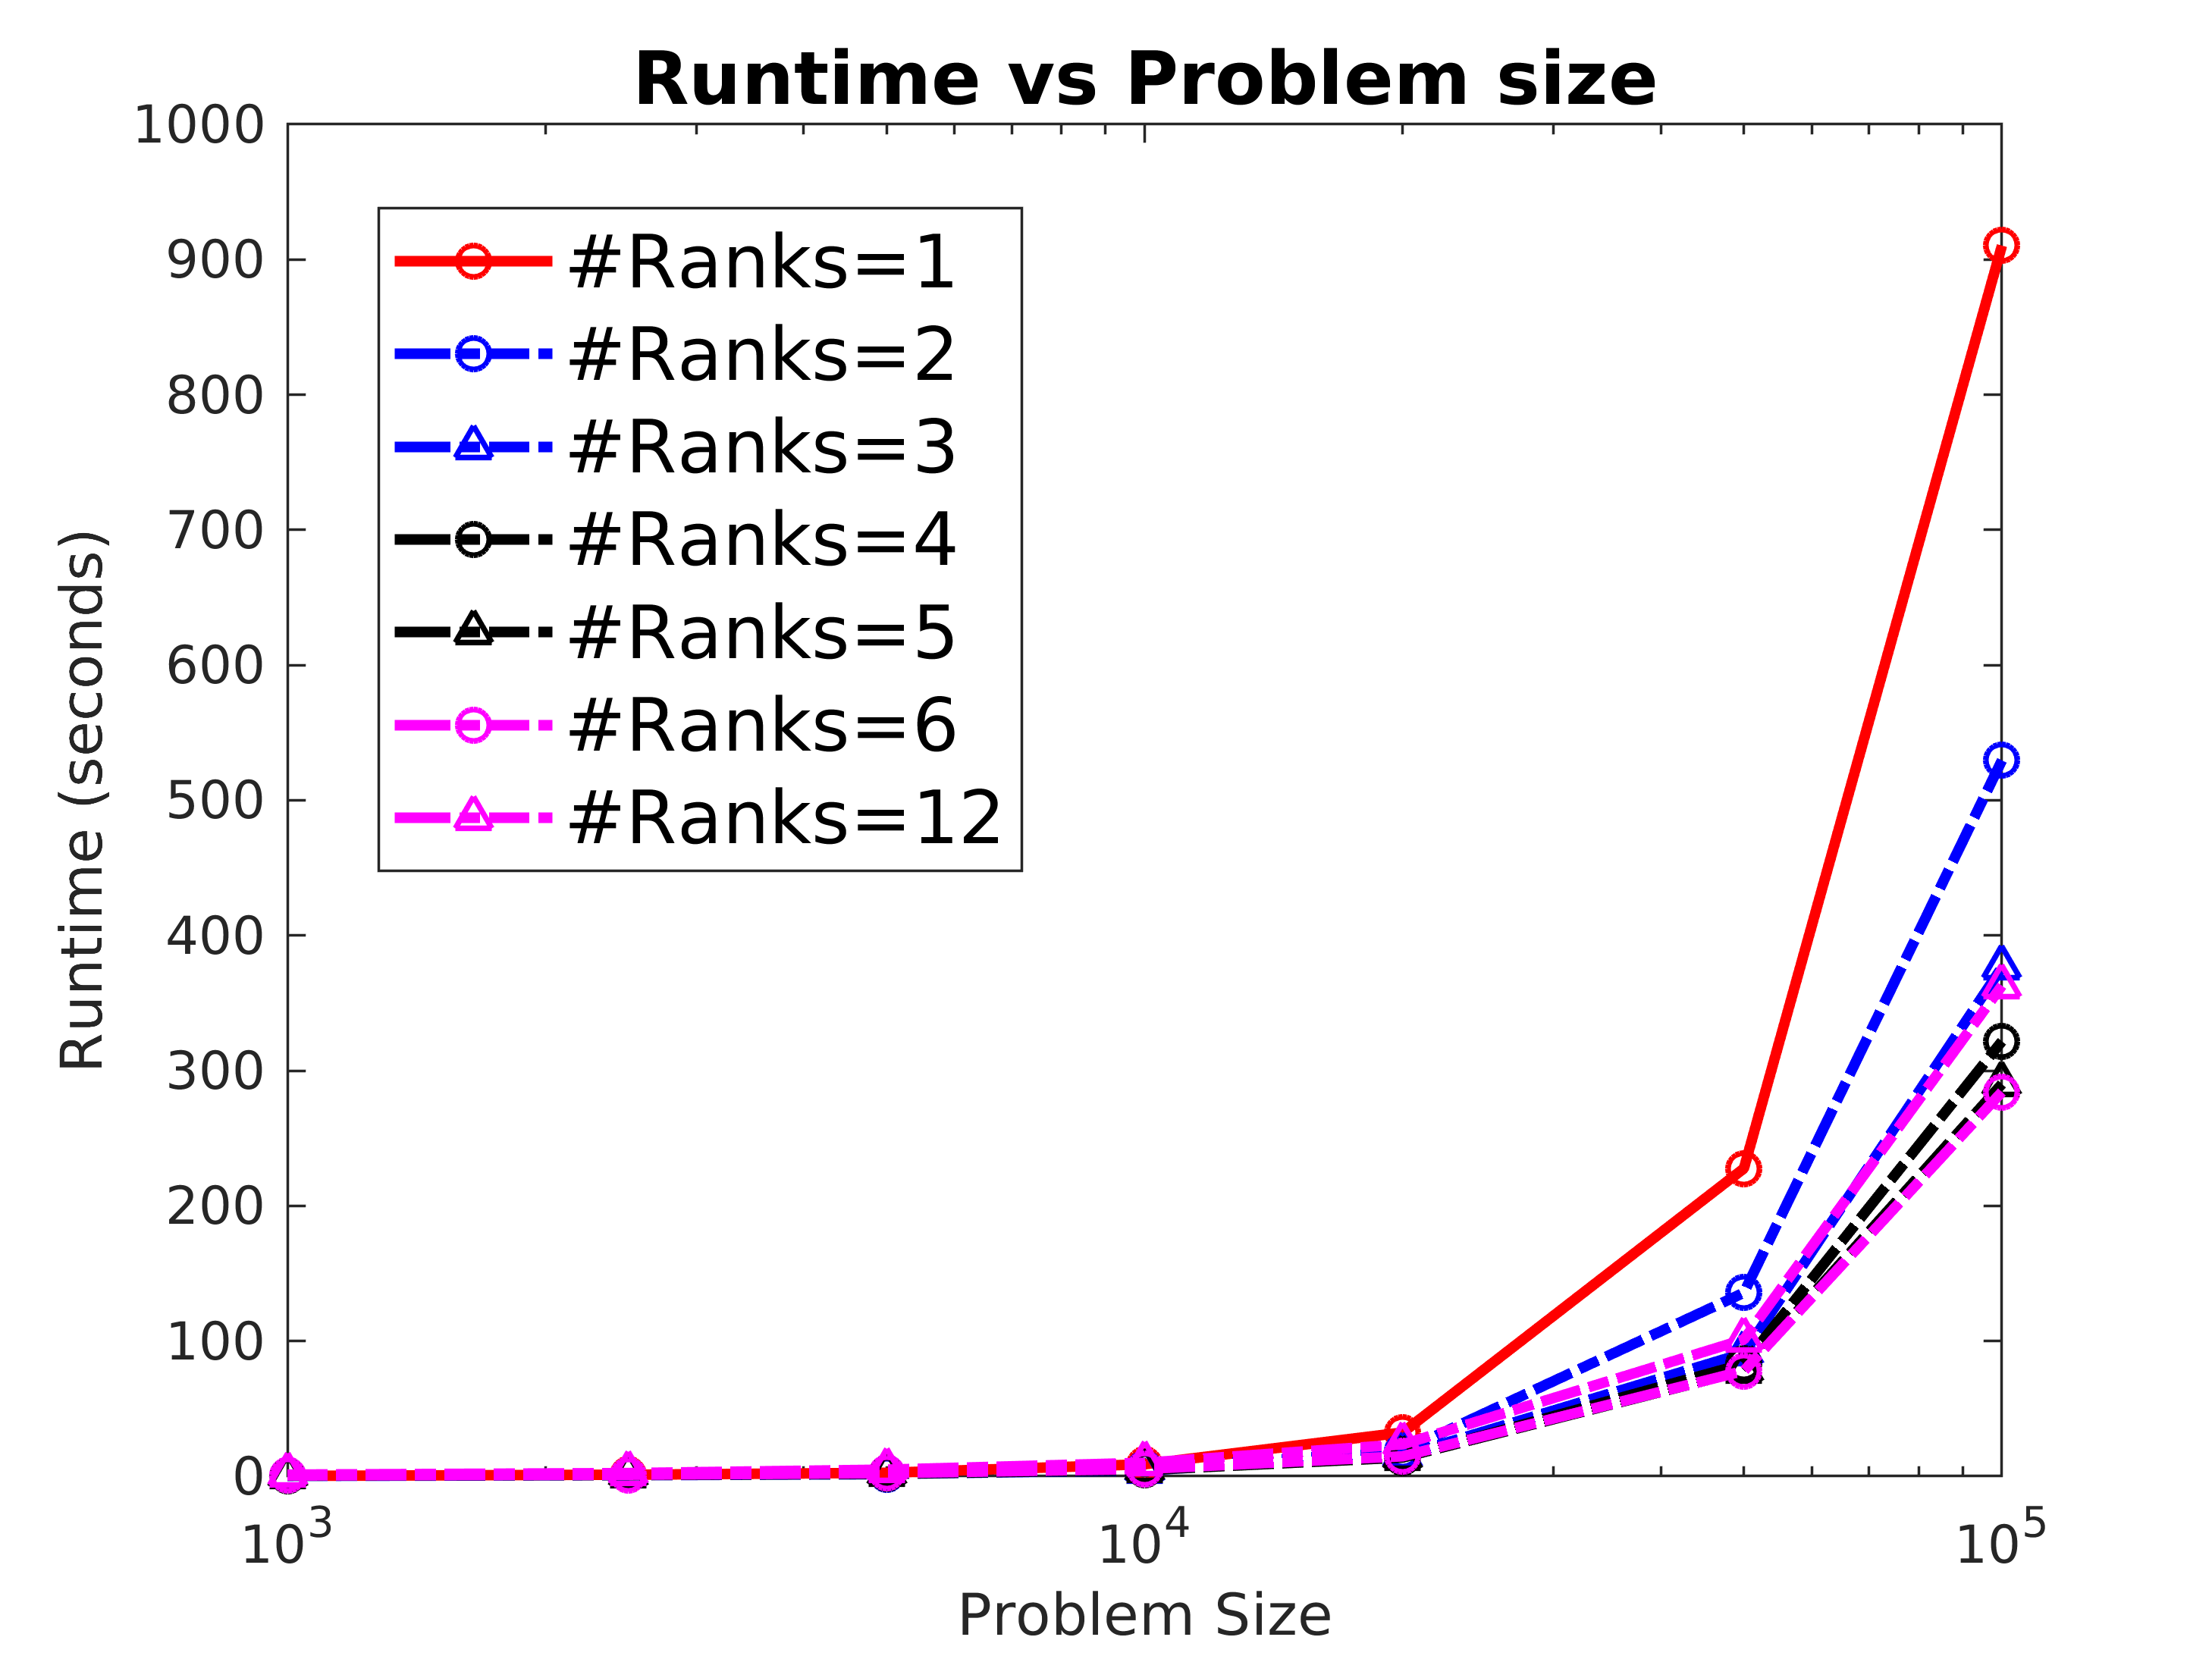
\includegraphics[trim= 10 5 35 10,clip, width=0.95\linewidth, height=5cm]{plots/MPI_weak_allrank.png} 
		\caption{Linear time scale}
	\end{subfigure}
	\begin{subfigure}{0.3\textwidth}
		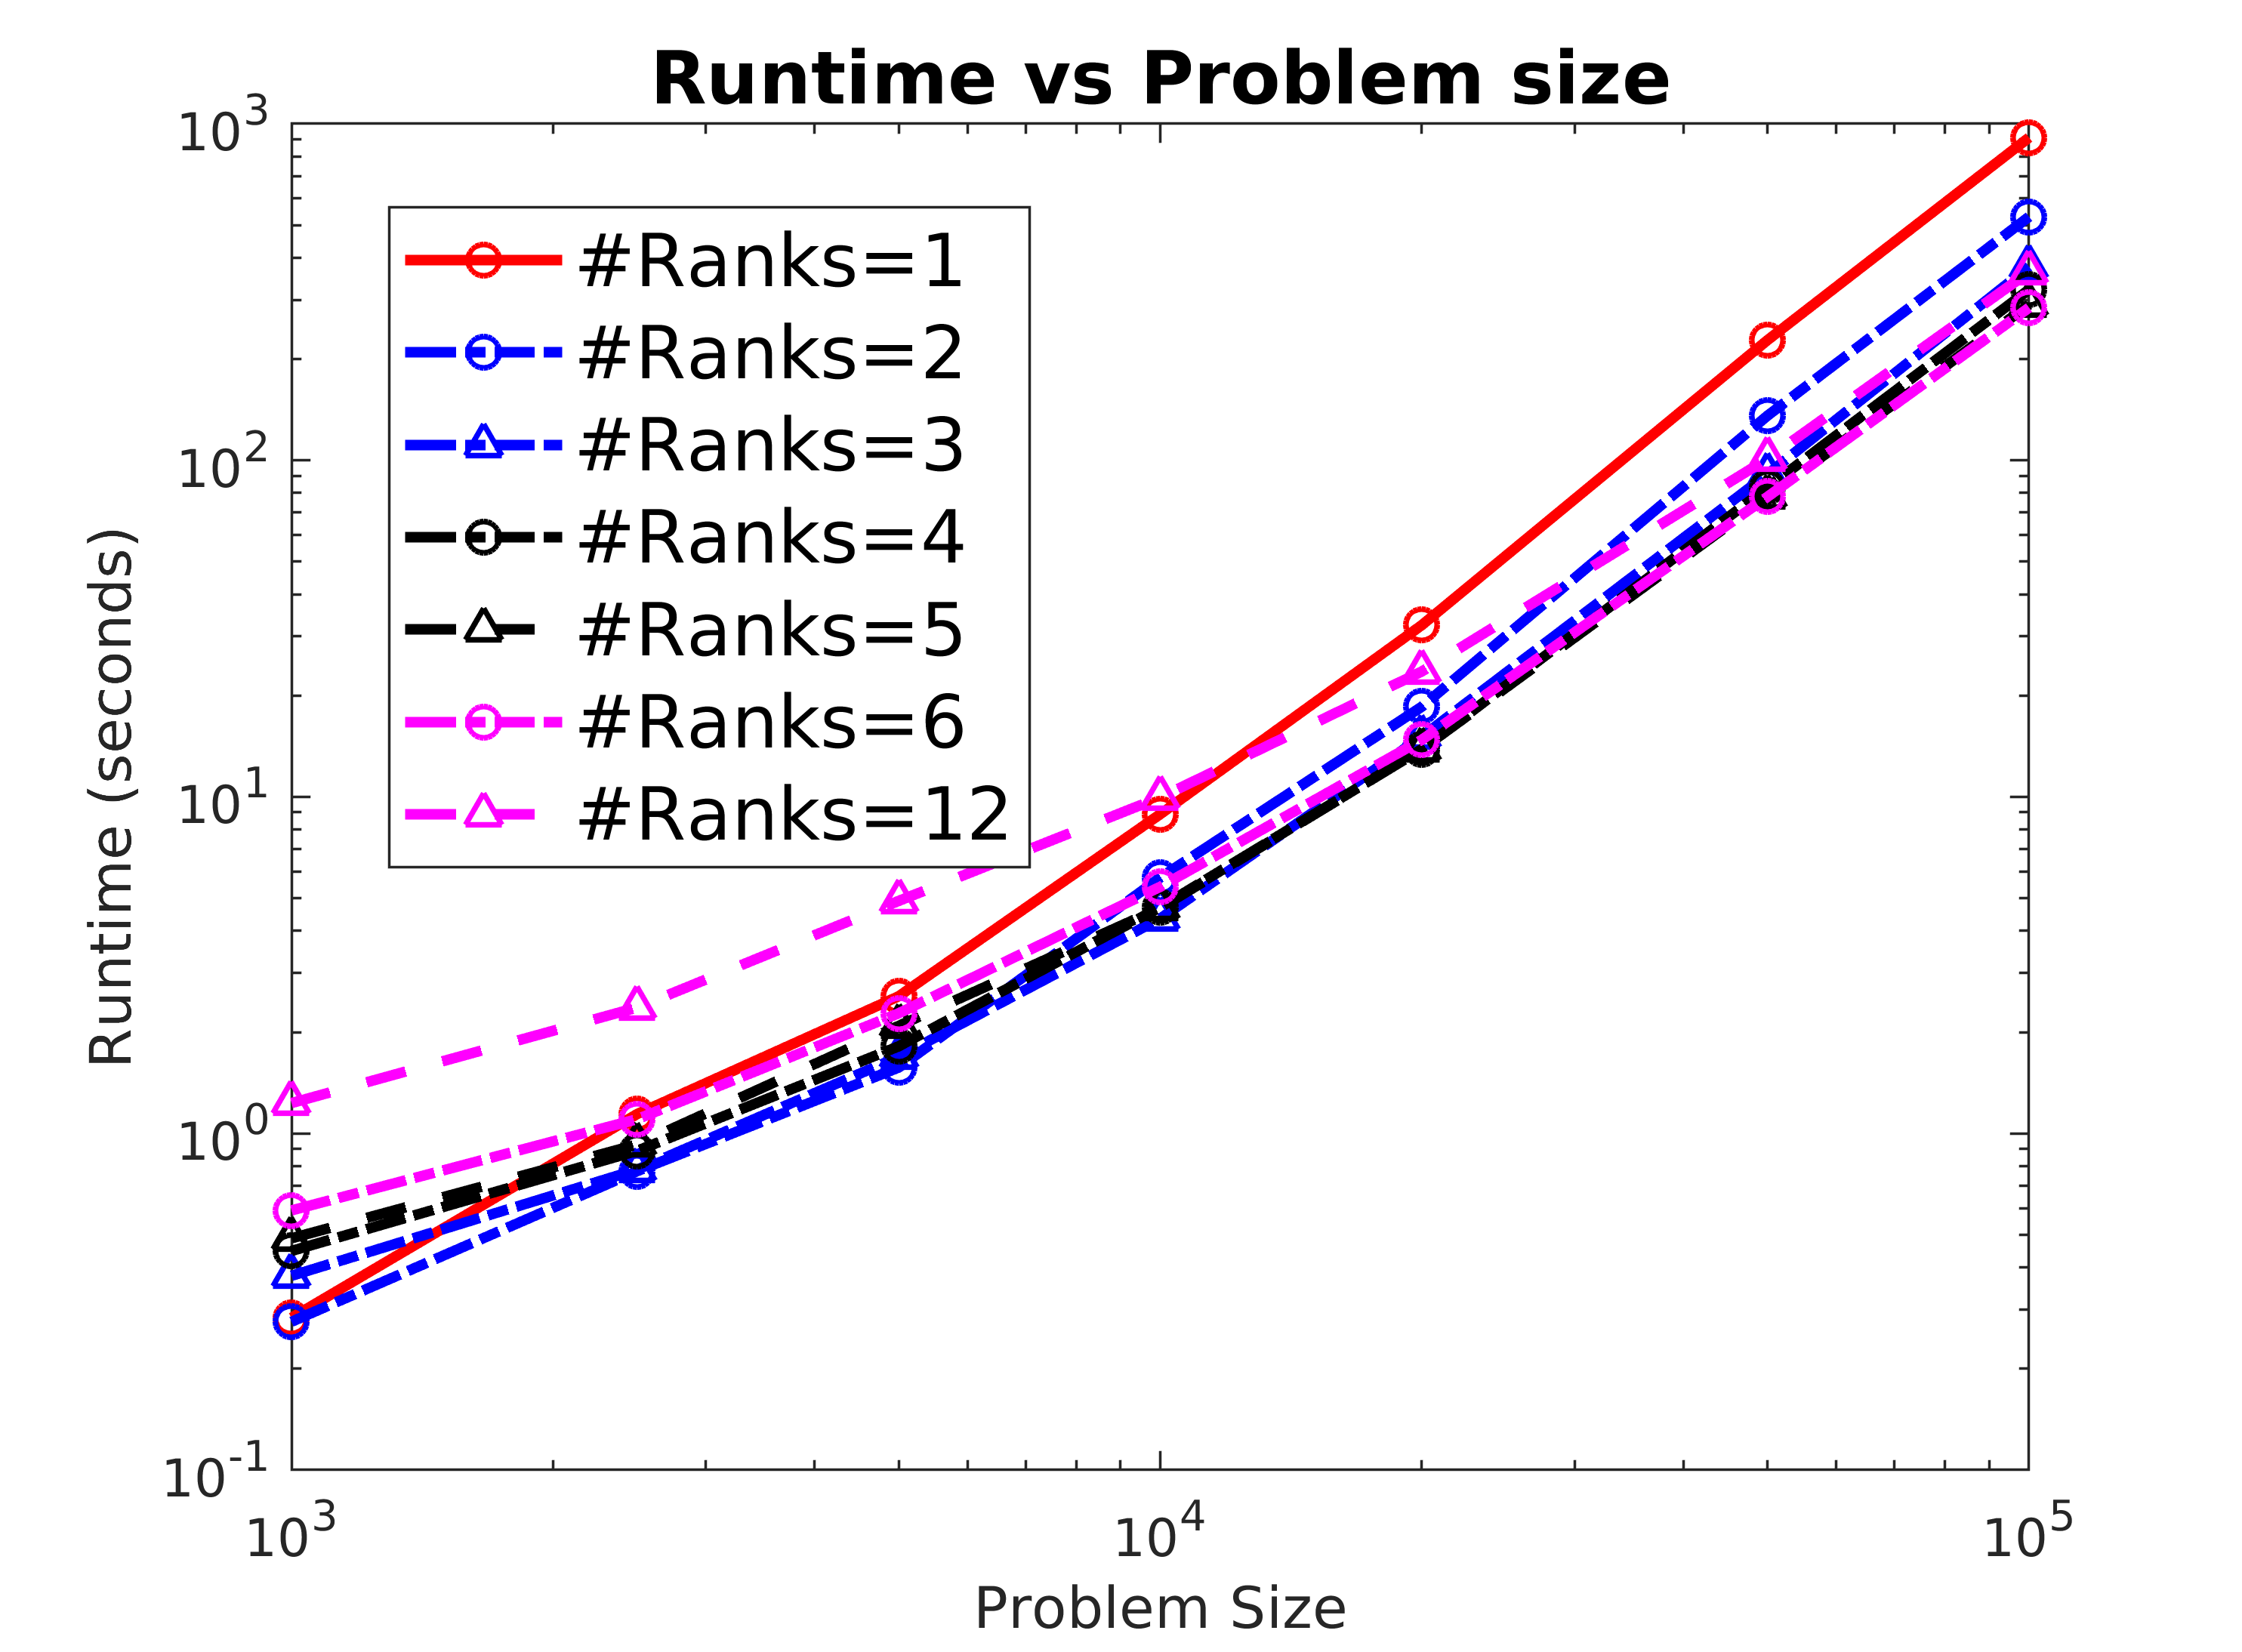
\includegraphics[trim= 10 5 35 10,clip, width=0.95\linewidth, height=5cm]{plots/MPI_weak_allrank_loglog.png}
		\caption{Log time scale}
	\end{subfigure}
	\caption{Run-time vs. problem size for all ranks}
	\label{weak}
\end{figure}

\noindent Weak scaling results from Fig. \ref{weak} show a greater \% increase in the speedup with increase in number of ranks for larger systems. 

\subsection{MPI/CUDA Performance}
Similar test cases as Section \ref{mpi_perfrom} are used to analyze the performance of the hybrid MPI/CUDA version of the solver. The results for both versions are also compared in this section. As explained in the Section \ref{cuda_dot}, we are employing a CUDA reduction technique for vector-dot product. We first analyze the performance gain obtained by using the reduction technique. 

\begin{figure}
	\begin{subfigure}{0.3\textwidth}
		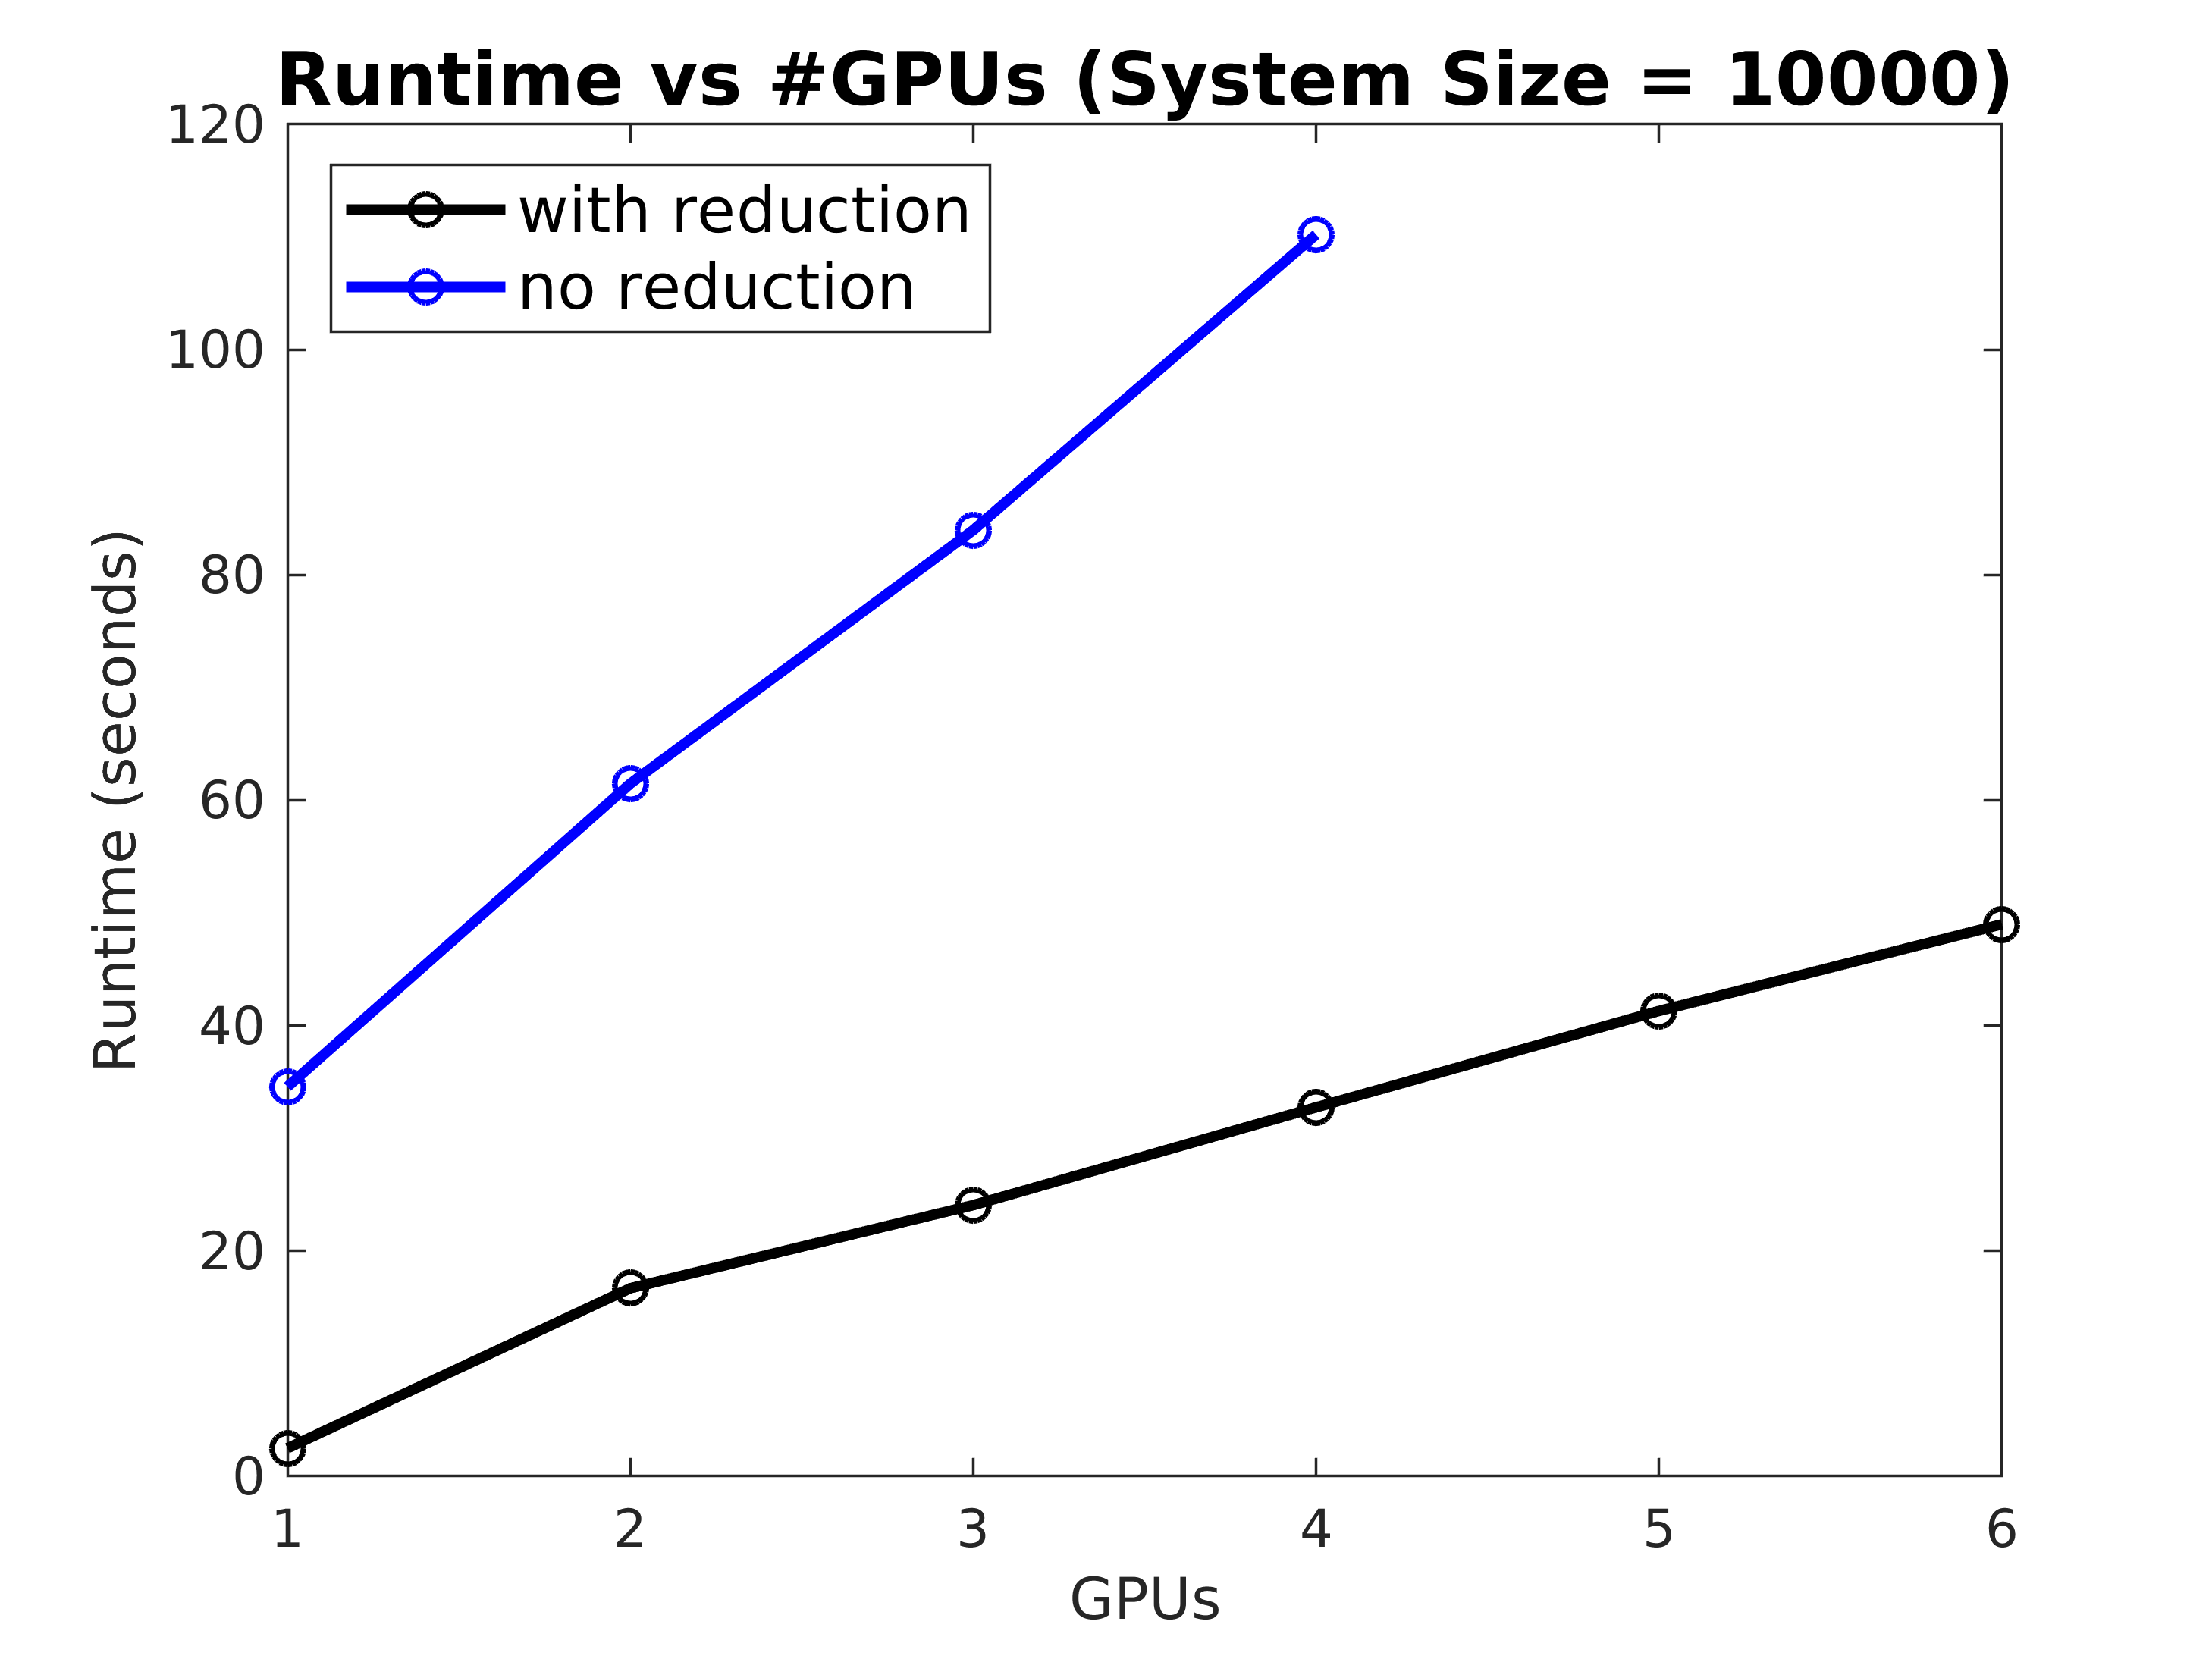
\includegraphics[trim= 10 5 35 10,clip, width=0.95\linewidth, height=5cm]{plots/CUDA_strong_10k.png} 
		\caption{}
	\end{subfigure}
	\begin{subfigure}{0.3\textwidth}
		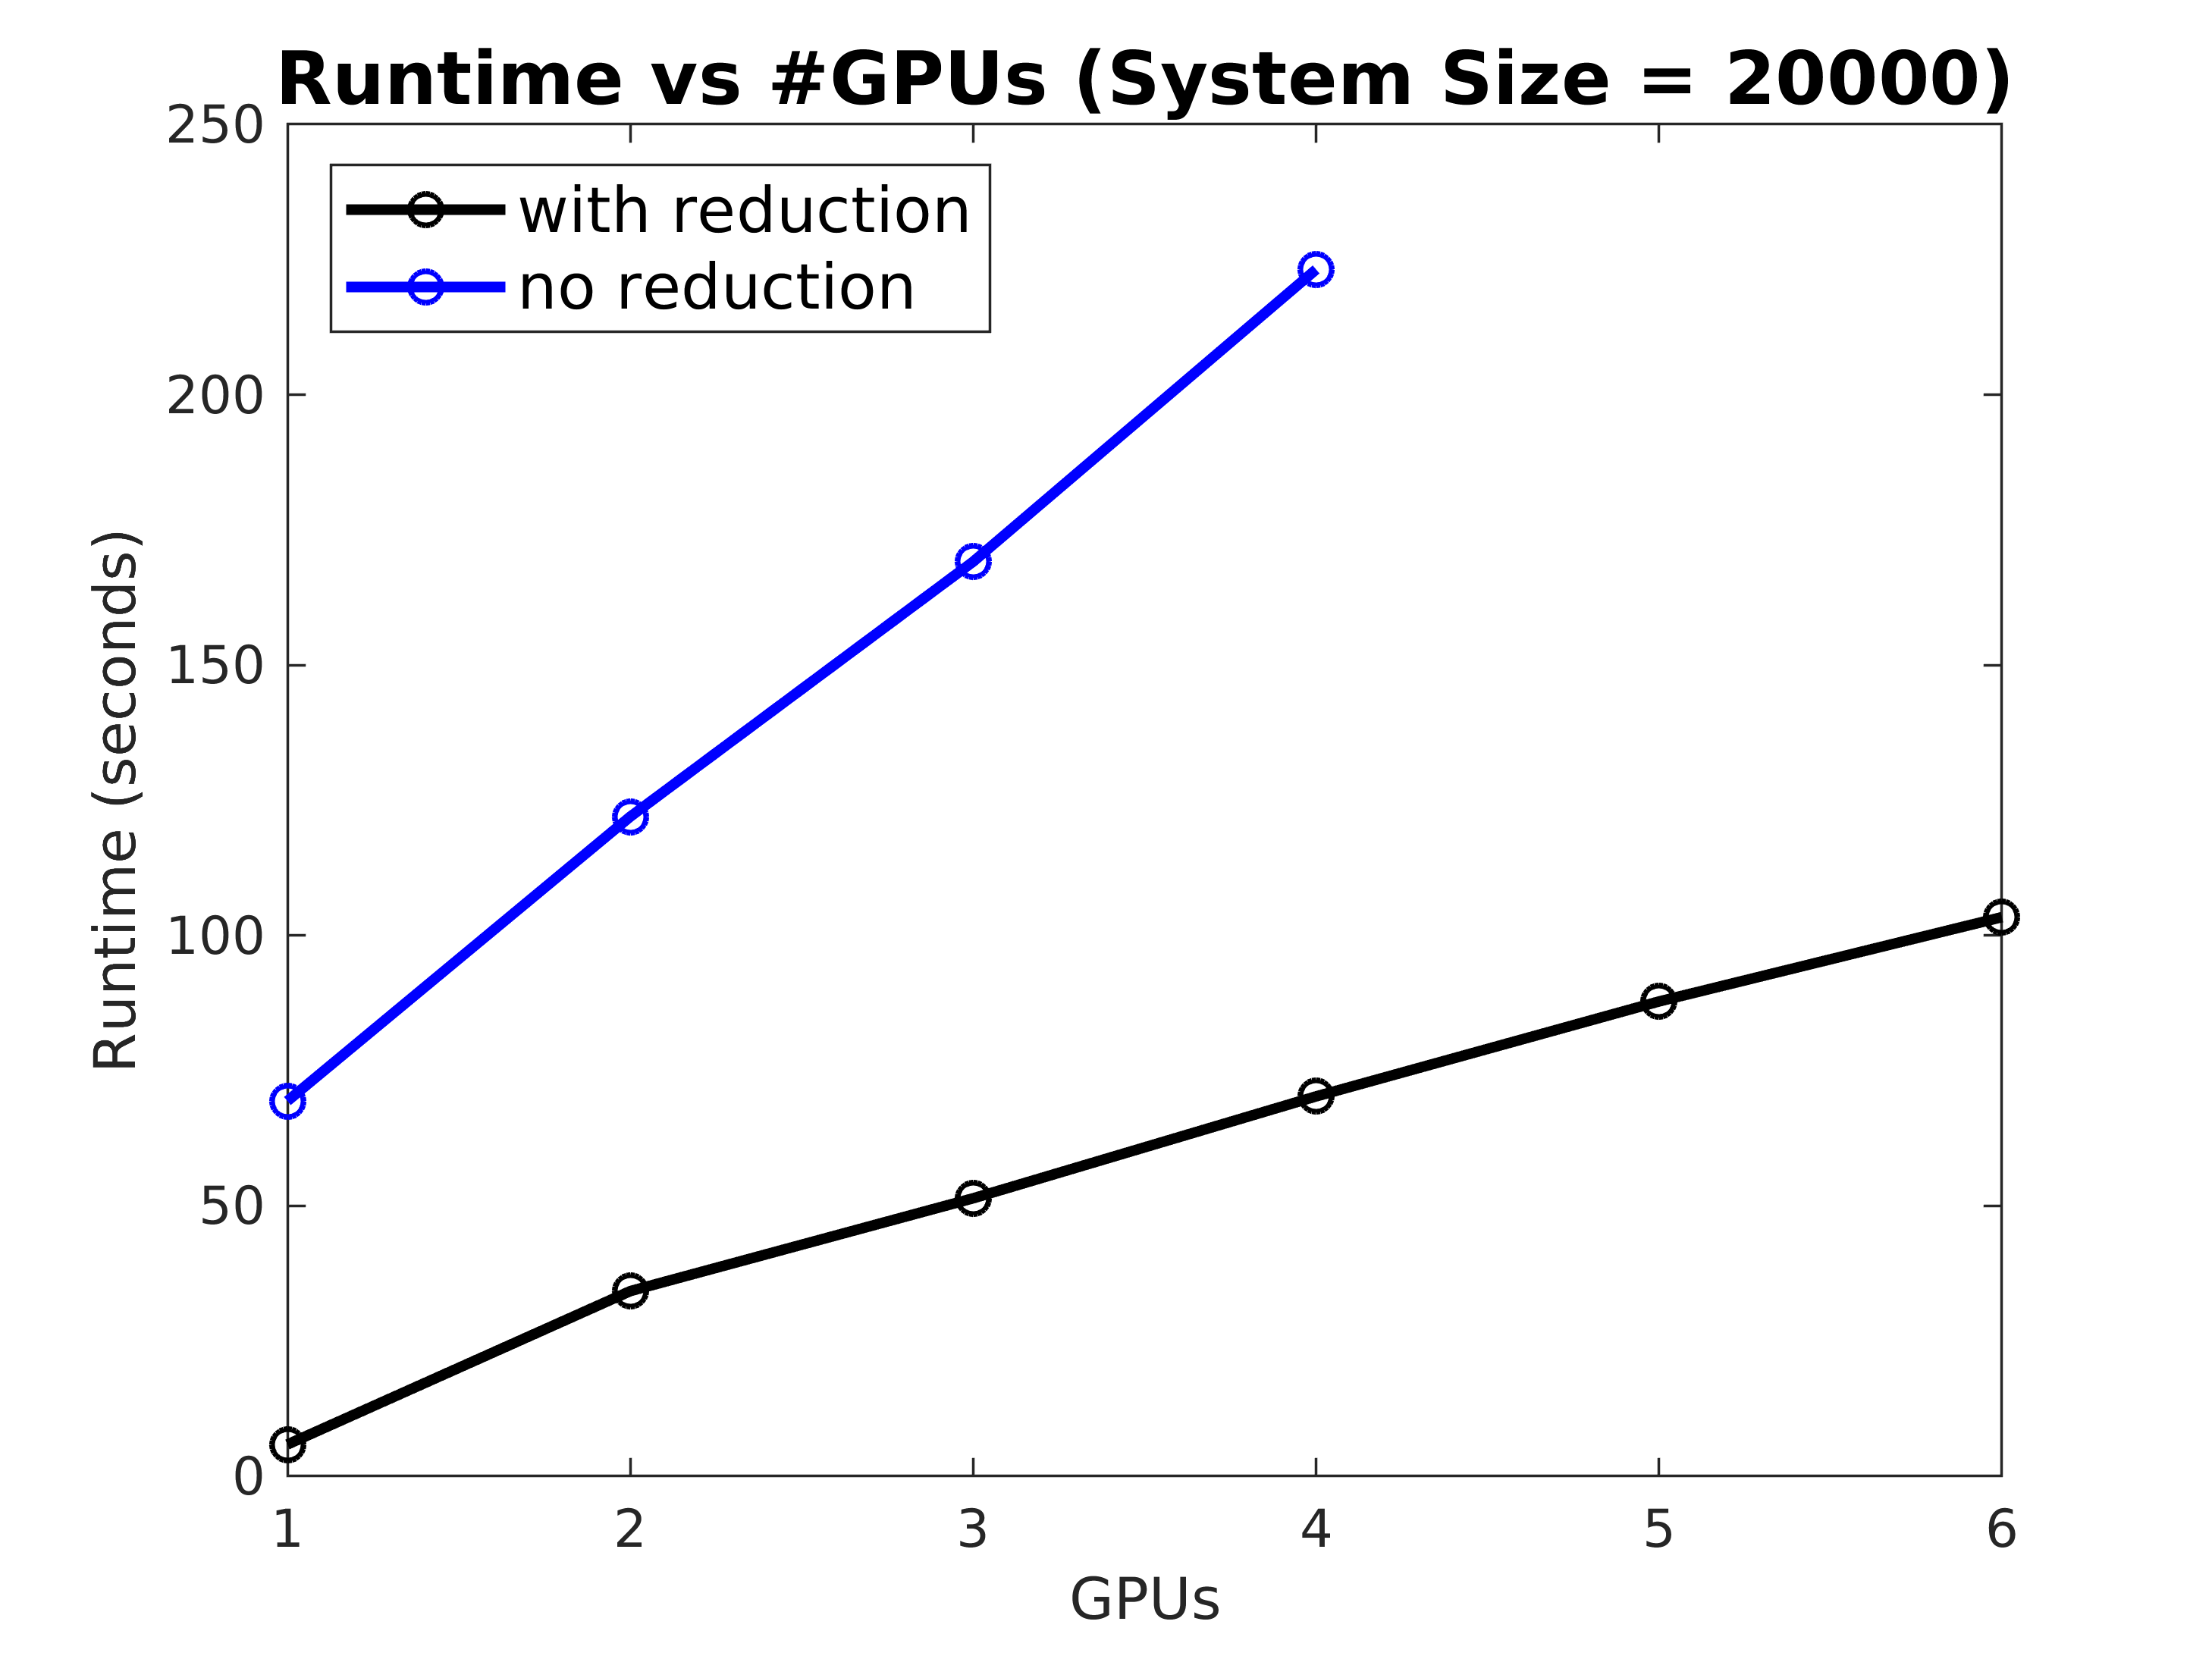
\includegraphics[trim= 10 5 35 10,clip, width=0.95\linewidth, height=5cm]{plots/CUDA_strong_20k.png}
		\caption{}
	\end{subfigure}
	\caption{Run-time comparison after applying reduction technique}
	\label{compare}
\end{figure}
Fig. \ref{compare} illustrates that the run-time significantly decreases after applying CUDA reduction technique for vector-dot product. All the subsequent MPI/CUDA results presented are with the reduction technique. 

Strong scaling studies for different systems are done on the hybrid solver. The run-time analysis vs. number of GPUs for all systems is presented in Fig. \ref{cuda-strong}. Also we compare theses results with the MPI only solver's performance. The comparison for   

\begin{figure}[h!]
	\begin{center}
		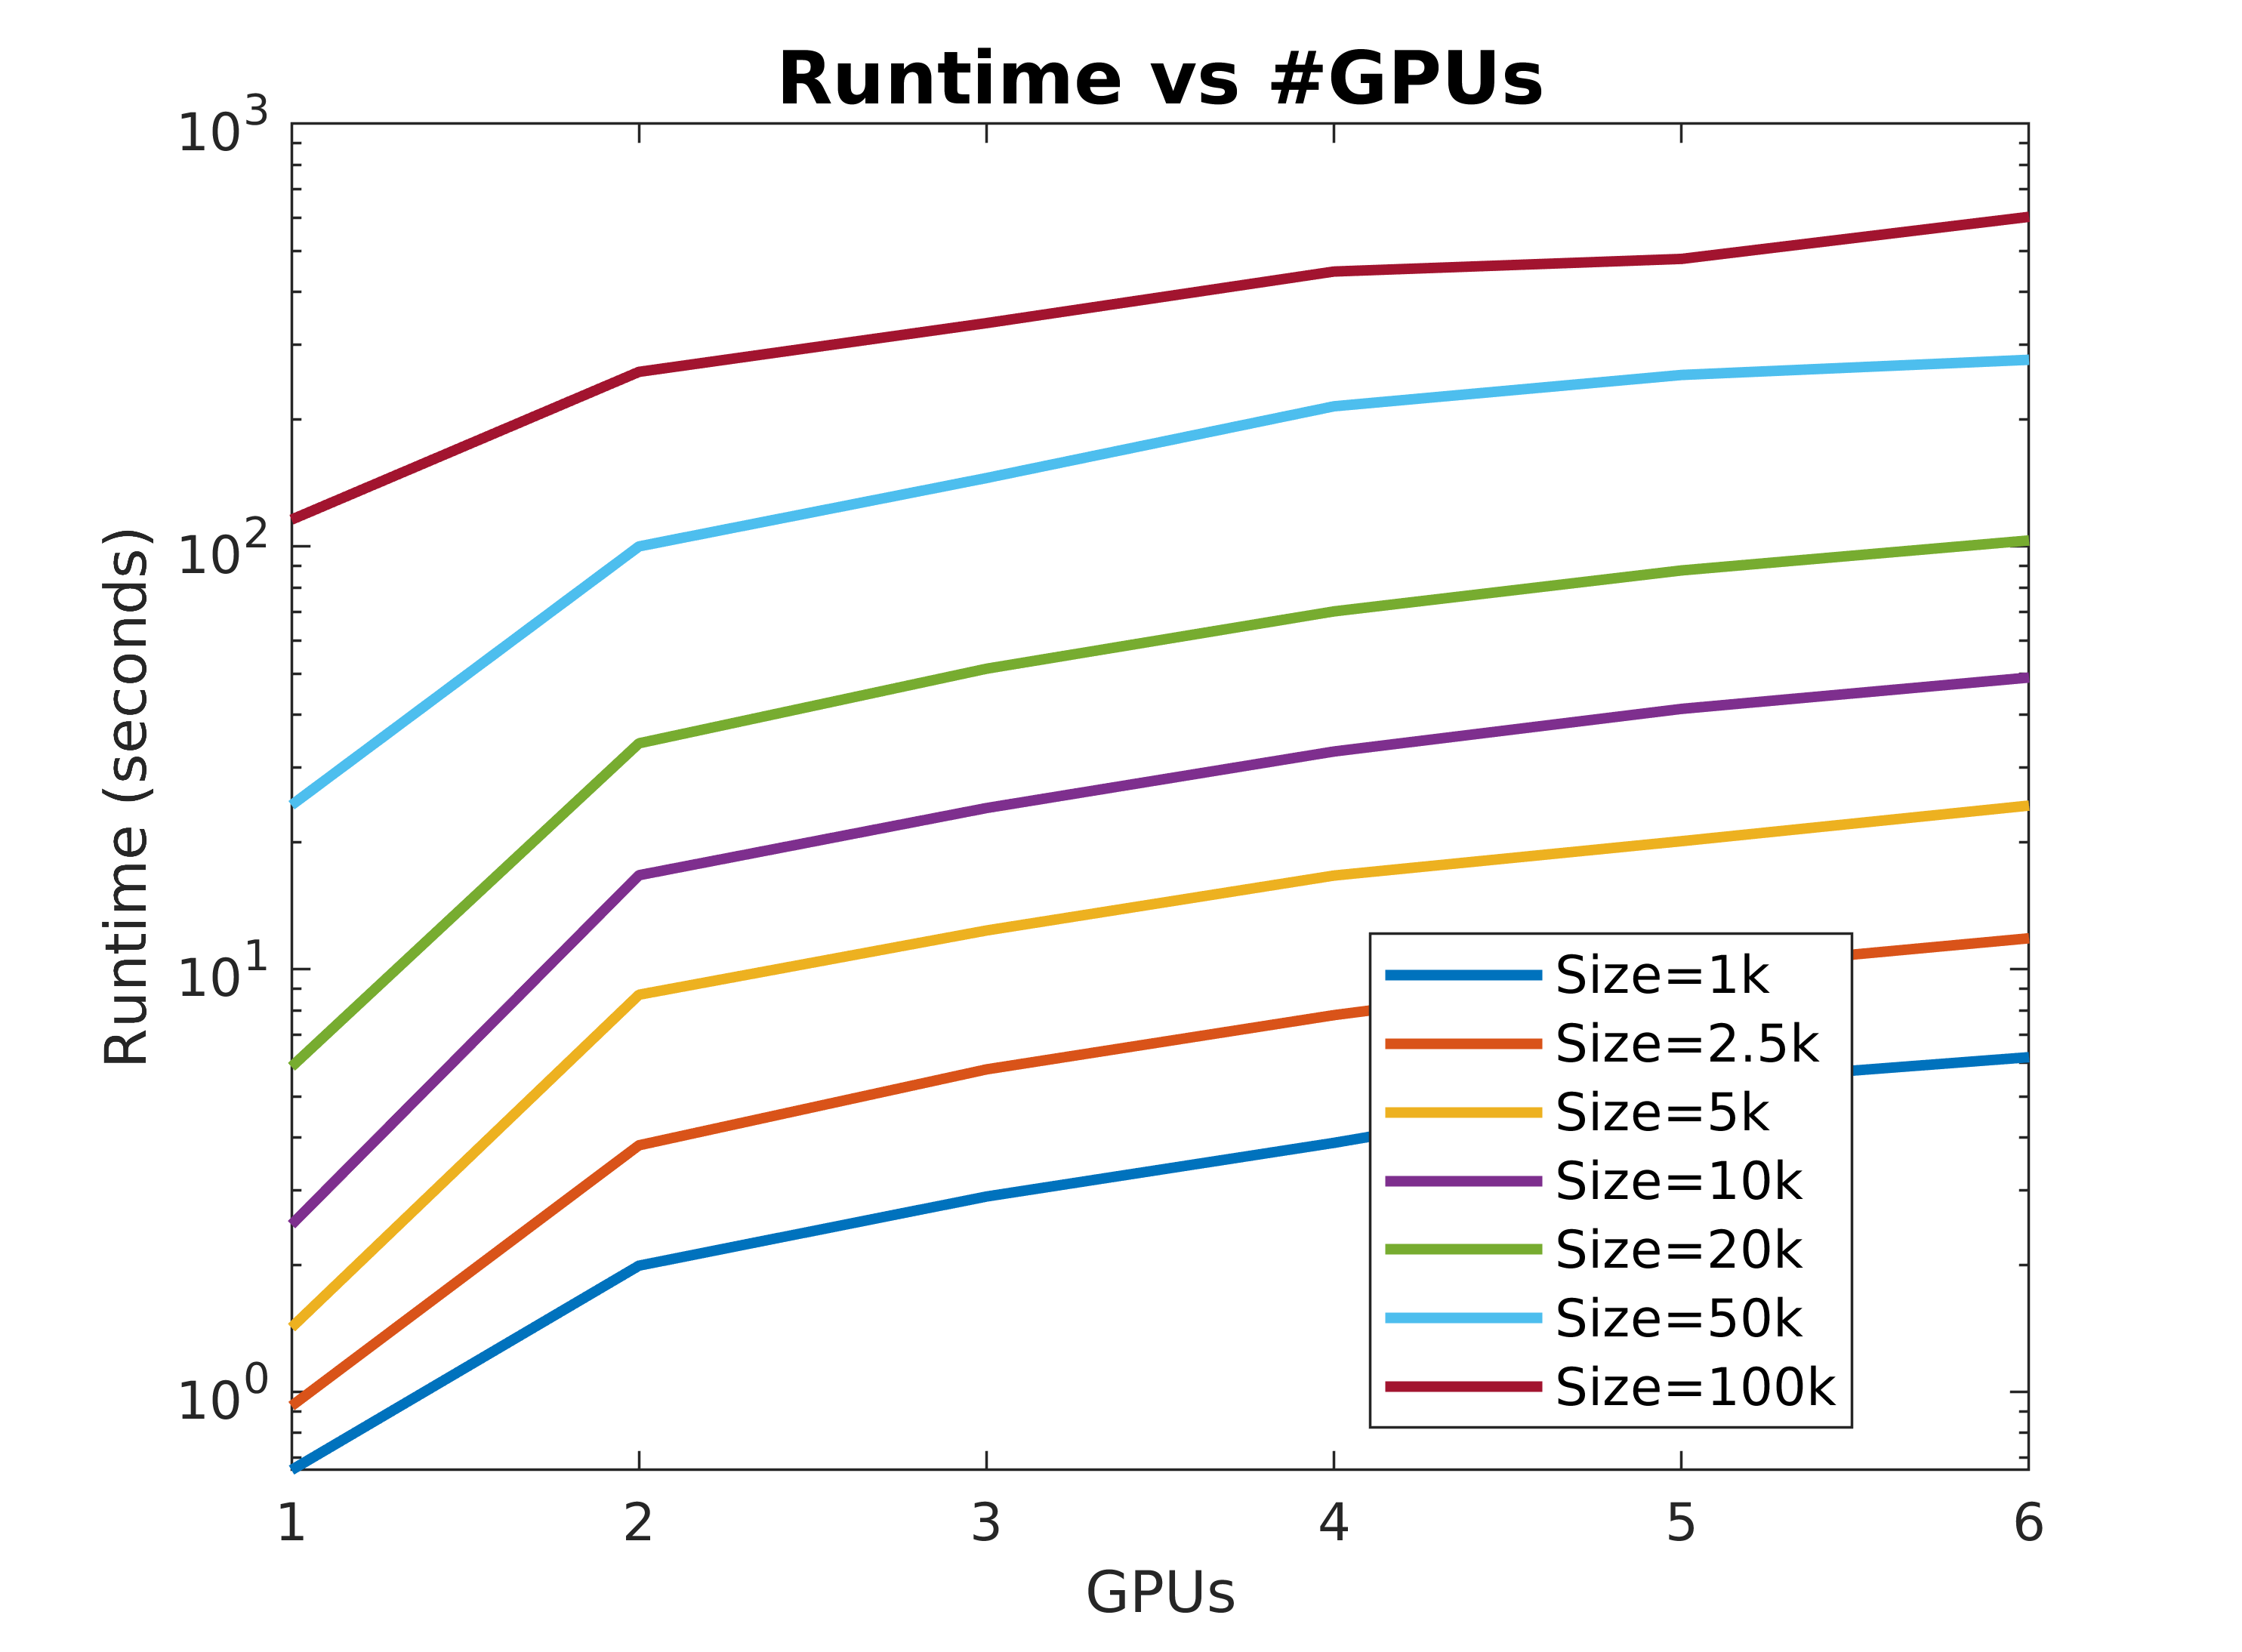
\includegraphics[width=0.35\textwidth]{plots/CUDA_strong_allranks_log.png}
	\end{center}
	\caption{Run-time vs. no. of GPUs for all cases}
	\label{cuda-strong}      
\end{figure}

\begin{figure}
	\begin{subfigure}{0.3\textwidth}
		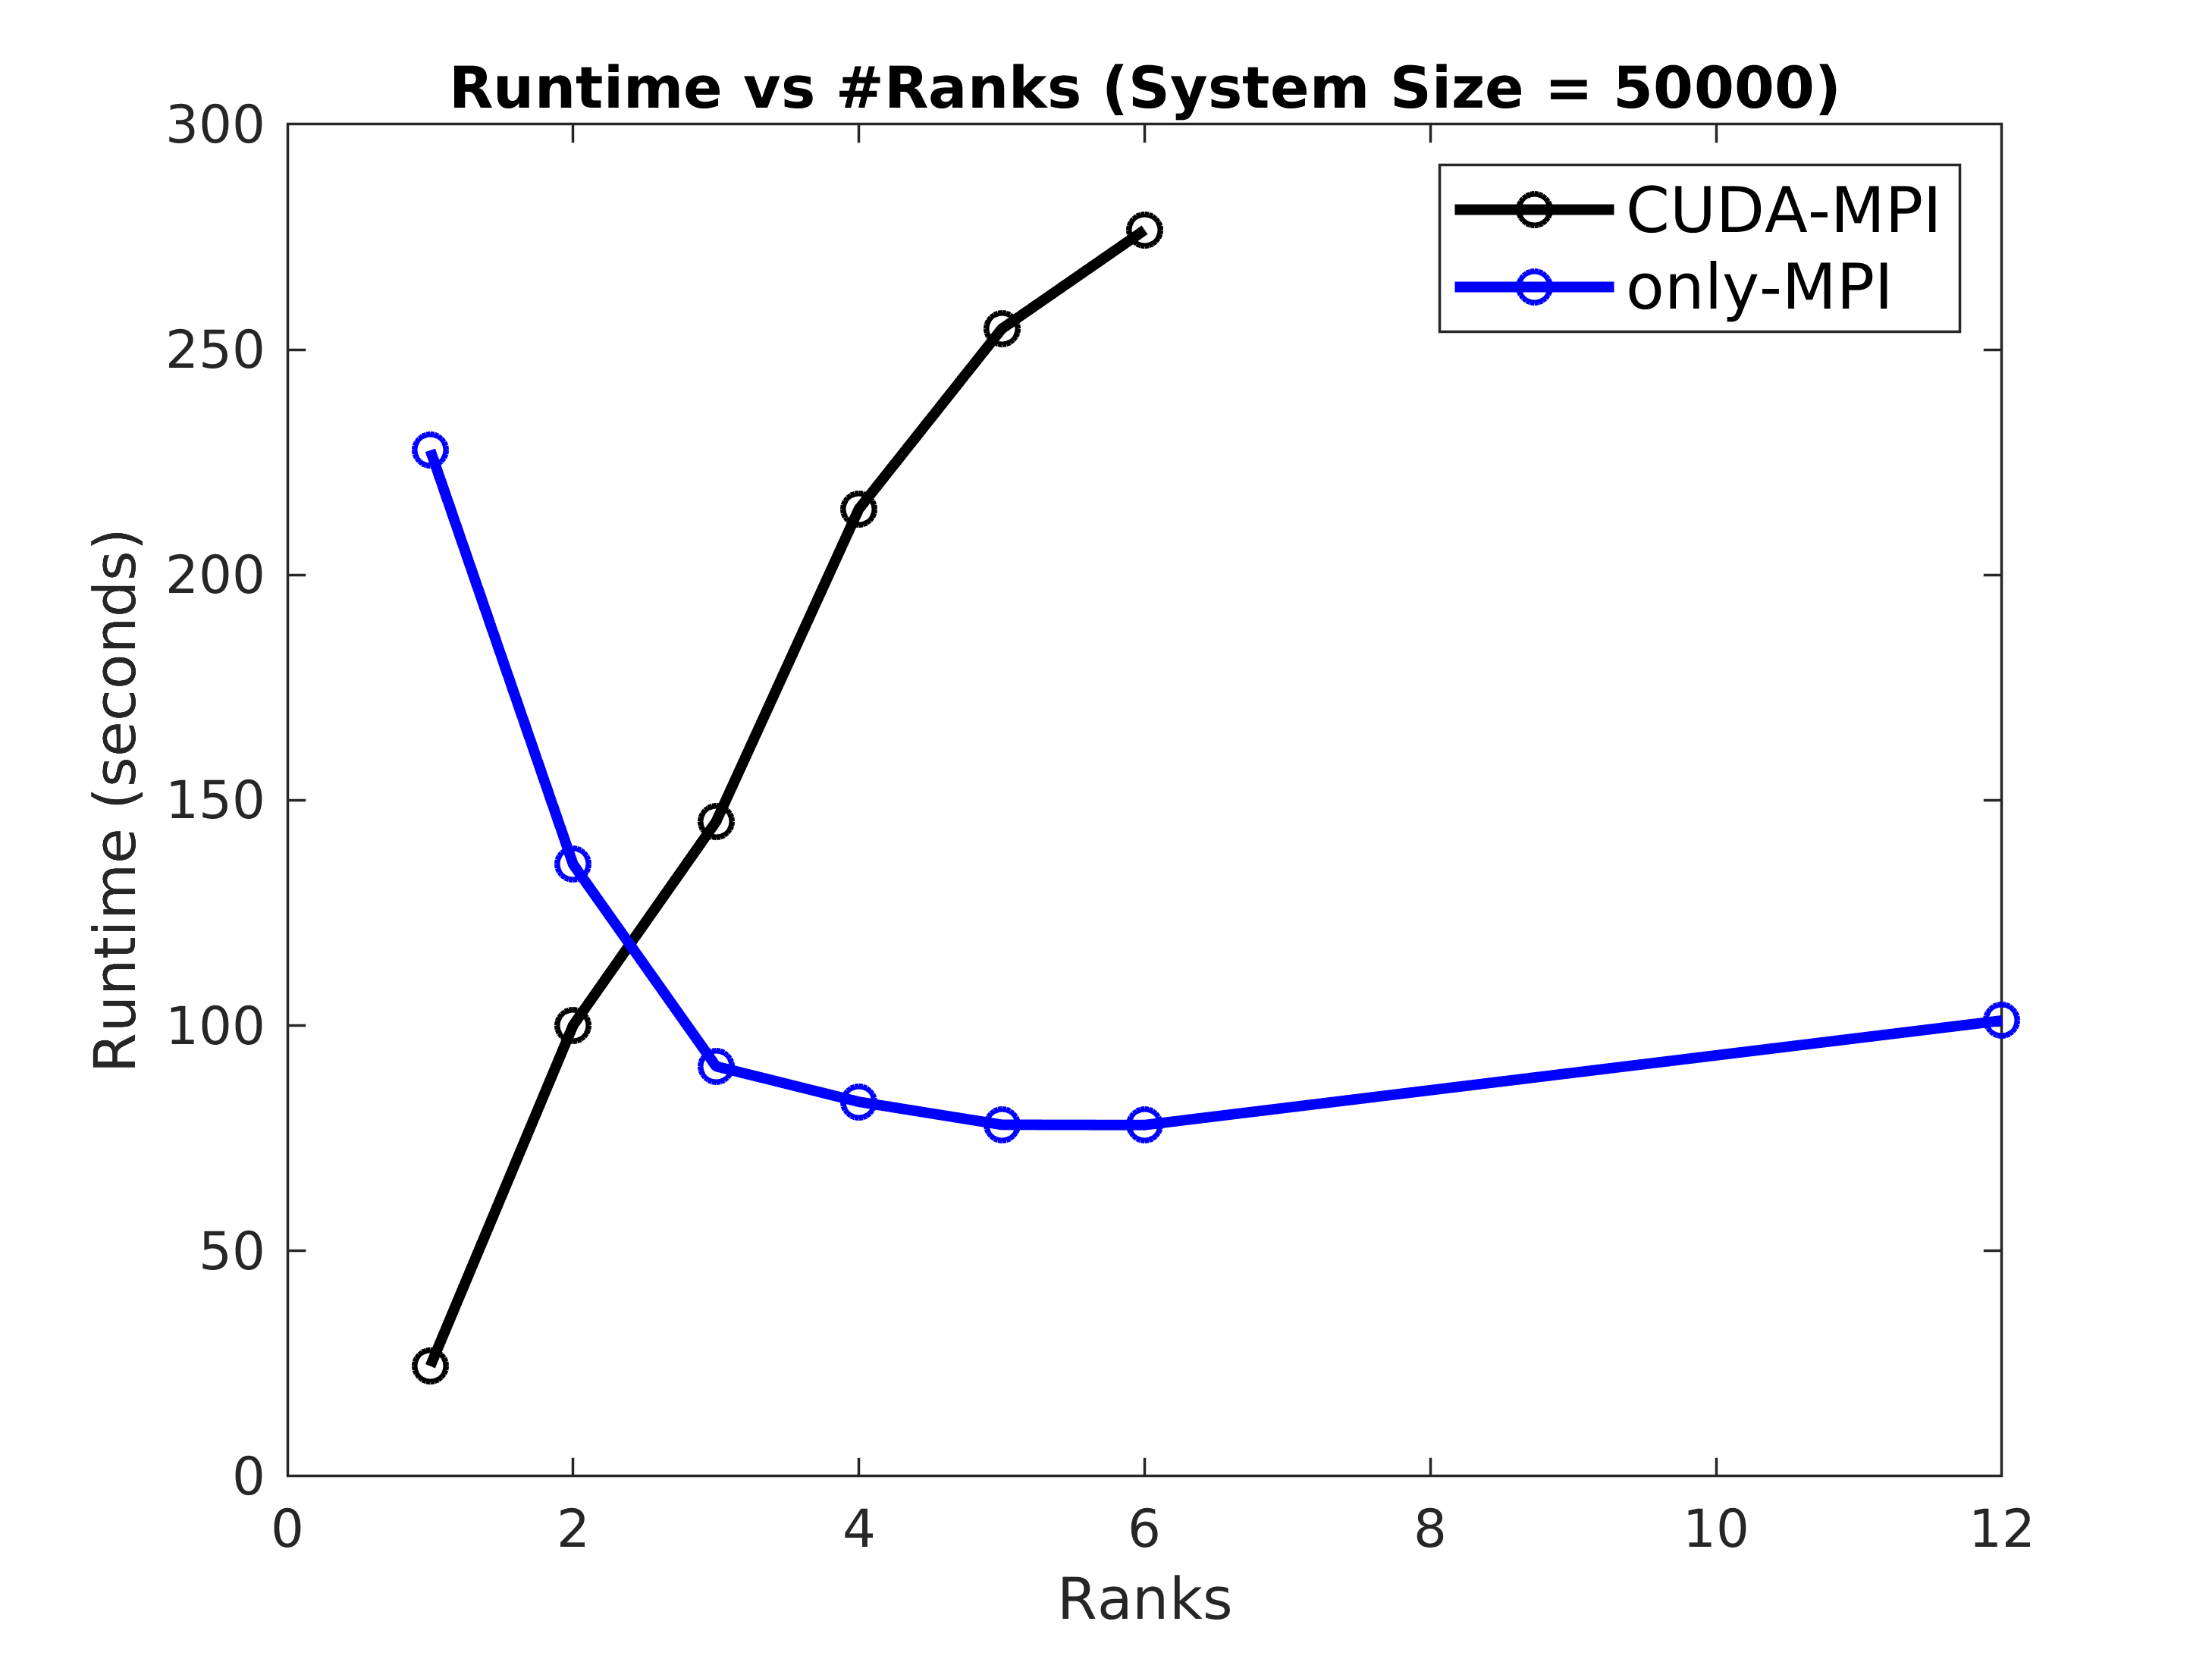
\includegraphics[trim= 10 5 35 10,clip, width=0.95\linewidth, height=5cm]{plots/compare_strong_50k.png} 
		\caption{}
	\end{subfigure}
	\begin{subfigure}{0.3\textwidth}
		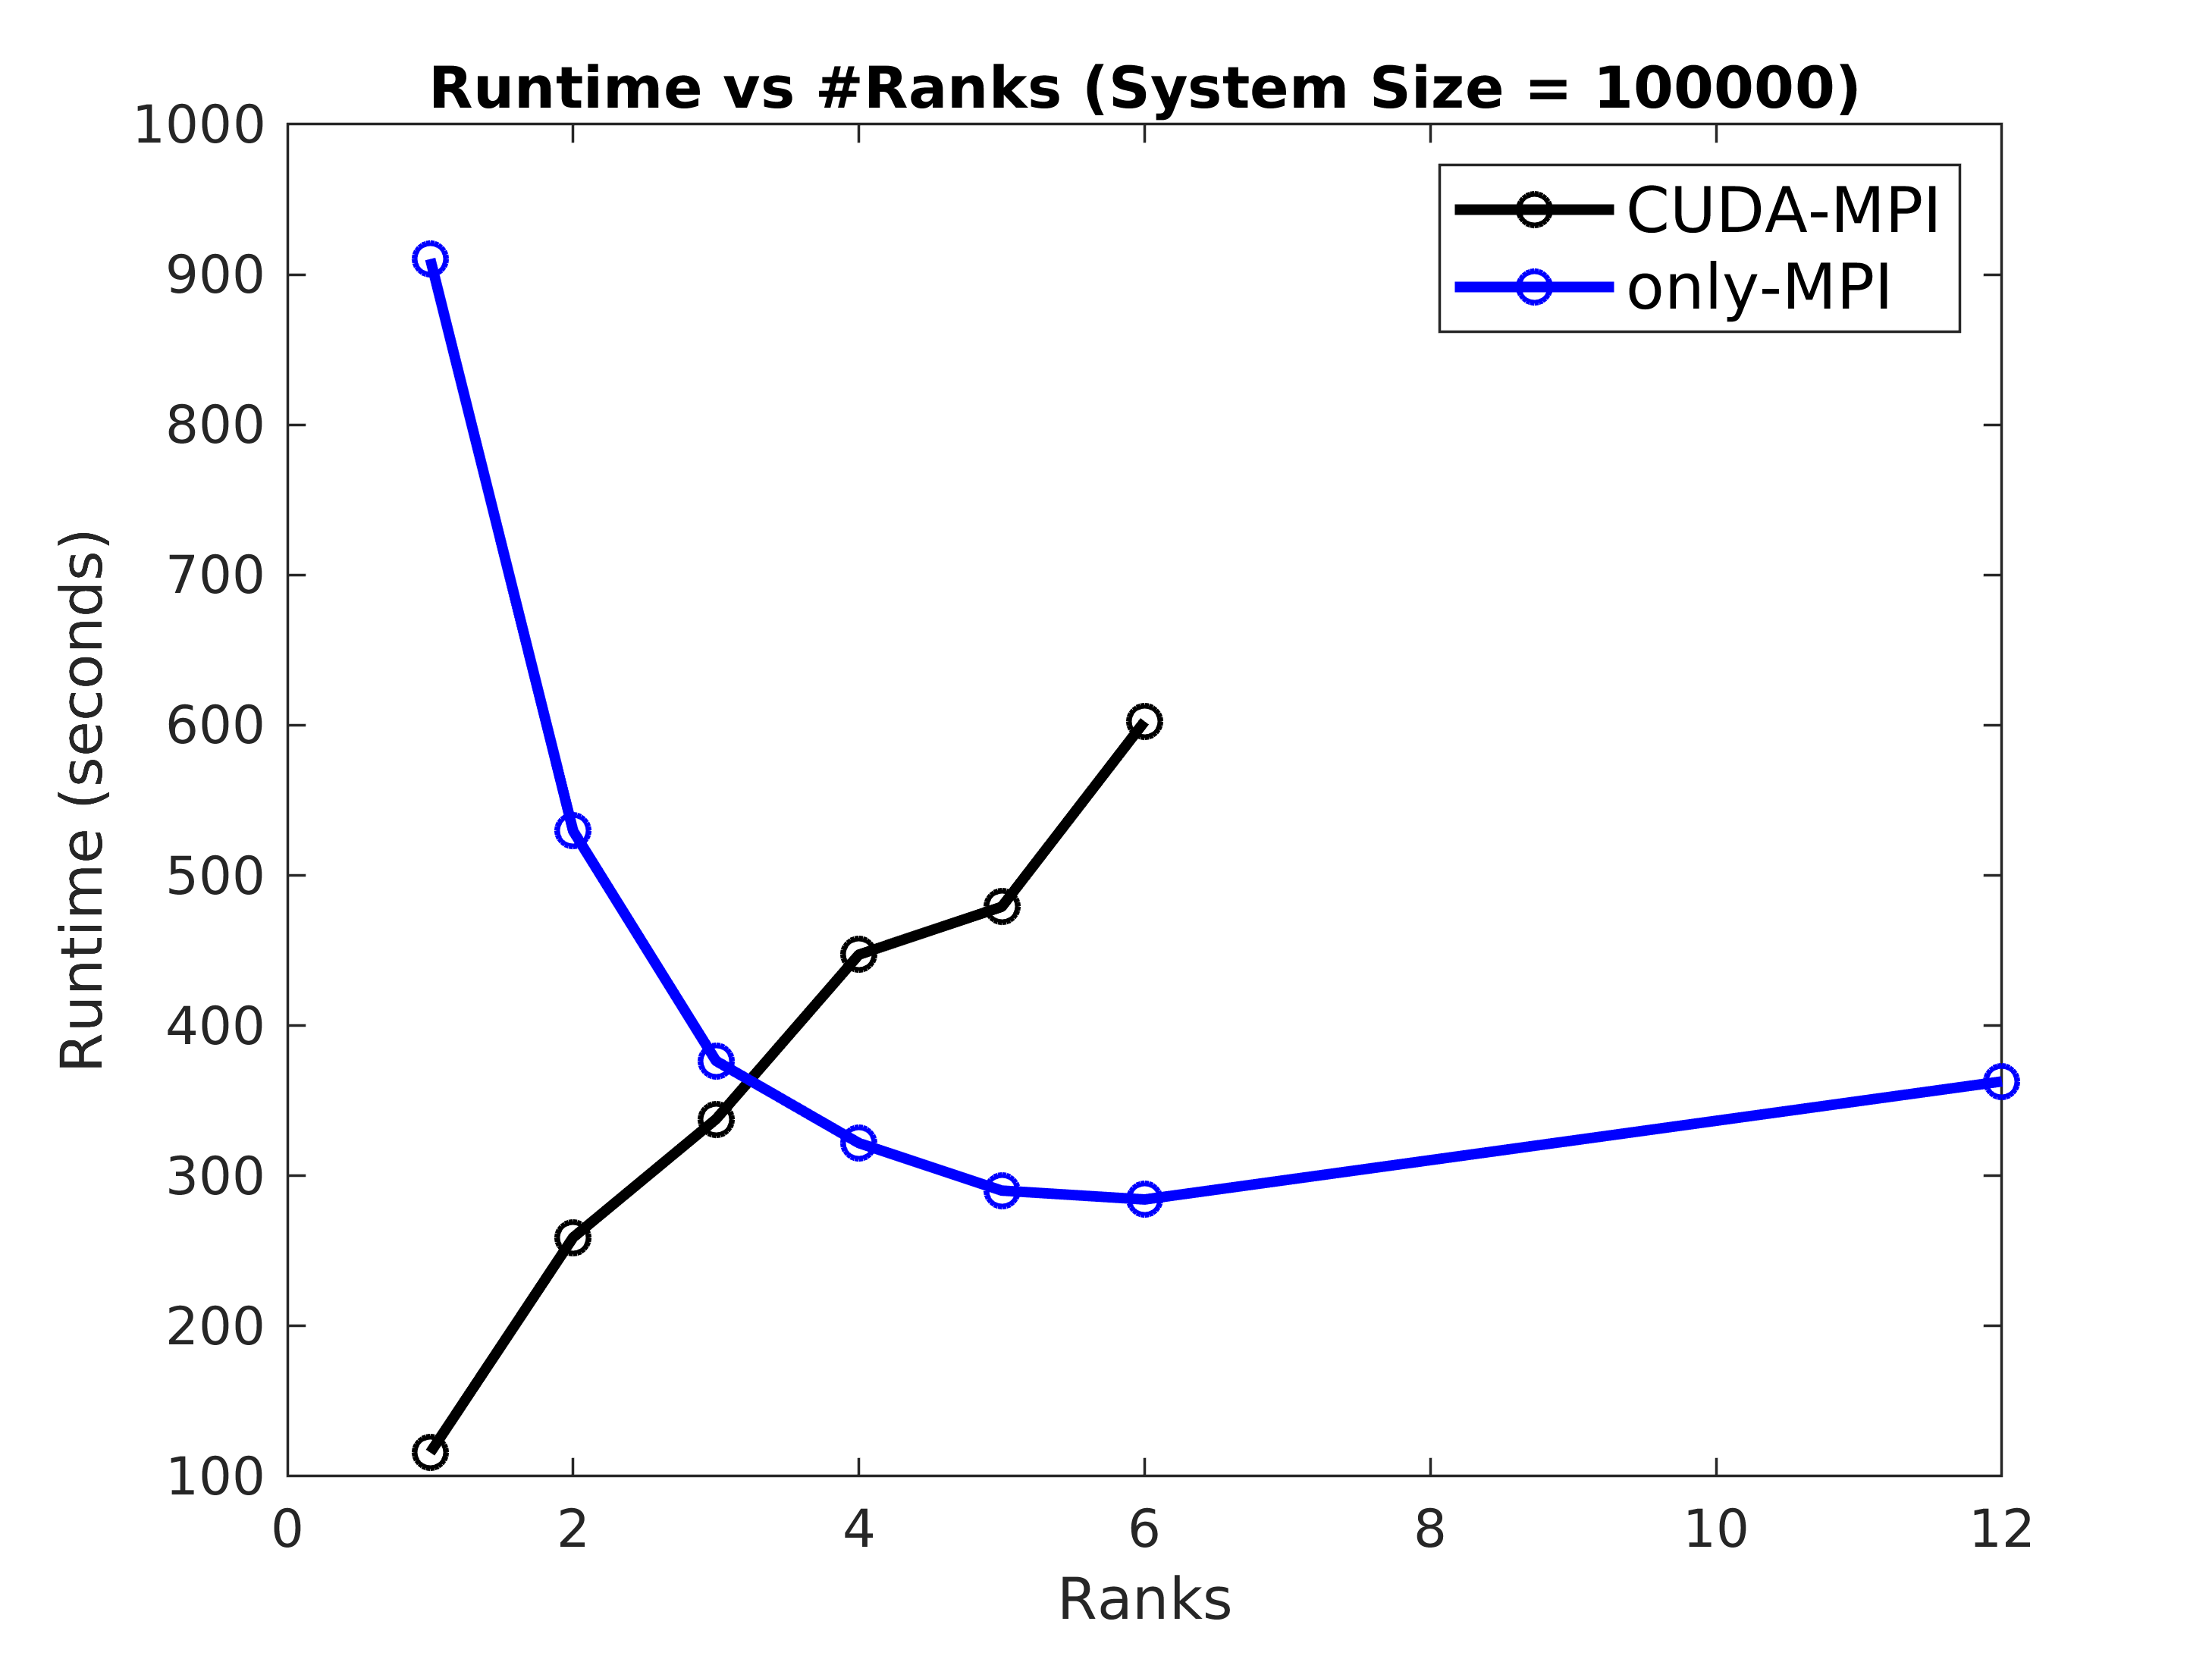
\includegraphics[trim= 10 5 35 10,clip, width=0.95\linewidth, height=5cm]{plots/compare_strong_100k.png}
		\caption{}
	\end{subfigure}
	\caption{Run-time comparison after applying reduction technique}
	\label{compare_strong}
\end{figure}


\subsection{Profiling}
\begin{table}[H]
	\scriptsize
	\caption{Profiling for 20k system size with 1 GPU}
	\label{tab:nvprof1}
	\begin{tabular}{|l|l|l|l|l|}
		\hline
		Rank               & \begin{tabular}[c]{@{}l@{}}\%\\ time\end{tabular} & \begin{tabular}[c]{@{}l@{}}self\\ seconds\end{tabular} & \begin{tabular}[c]{@{}l@{}}self\\ calls\end{tabular} & Kernel                         \\ \hline\hline
		\multirow{3}{*}{0} & 62.34                                             & 1.93                                                   & 60003                                                & dot\_product \\ \cline{2-5} 
		& 28.66                                             & 0.89                                                   & 60003                                                & vector\_addition                   \\ \cline{2-5} 
		& 9.00                                              & 0.28                                                   & 20002                                                & matrix\_vector\_multiplication               \\ \hline
	\end{tabular}
\end{table}


\begin{table}[H]
	\scriptsize
	\caption{Profiling for 20k system size with 2 GPU}
	\label{tab:nvprof2}
	\begin{tabular}{|l|l|l|l|l|}
		\hline
		Rank               & \begin{tabular}[c]{@{}l@{}}\%\\ time\end{tabular} & \begin{tabular}[c]{@{}l@{}}self\\ seconds\end{tabular} & \begin{tabular}[c]{@{}l@{}}self\\ calls\end{tabular} & Kernel                         \\ \hline\hline
		\multirow{3}{*}{0} & 63.43                                             & 3.71                                                   & 20002                                                & matrix\_vector\_multiplication \\ \cline{2-5} 
		& 27.69                                             & 1.62                                                   & 60003                                                & dot\_product                   \\ \cline{2-5} 
		& 8.88                                              & 0.52                                                   & 60003                                                & vector\_addition               \\ \hline\hline
		\multirow{3}{*}{1} & 61.25                                             & 3.71                                                   & 20002                                                & matrix\_vector\_multiplication \\ \cline{2-5} 
		& 27.73                                             & 1.68                                                   & 60003                                                & dot\_product                   \\ \cline{2-5} 
		& 11.02                                              & 0.67                                                   & 60003                                                & vector\_addition               \\ \hline
	\end{tabular}
\end{table}


\begin{table}[H]
	\scriptsize
	\caption{Profiling for 20k system size with 6 GPU}
	\label{tab:nvprof3}
	\begin{tabular}{|l|l|l|l|l|}
		\hline
		Rank               & \begin{tabular}[c]{@{}l@{}}\%\\ time\end{tabular} & \begin{tabular}[c]{@{}l@{}}self\\ seconds\end{tabular} & \begin{tabular}[c]{@{}l@{}}self\\ calls\end{tabular} & Kernel                         \\ \hline\hline
		\multirow{3}{*}{0} & 72.84                                             & 5.01                                                   & 20002                                                & matrix\_vector\_multiplication \\ \cline{2-5} 
		& 21.15                                             & 1.45                                                   & 60003                                                & dot\_product                   \\ \cline{2-5} 
		& 6.01                                              & 0.41                                                   & 60003                                                & vector\_addition               \\ \hline\hline
		\multirow{3}{*}{2} & 67.13                                             & 3.76                                                   & 20002                                                & matrix\_vector\_multiplication \\ \cline{2-5} 
		& 26.05                                             & 1.46                                                   & 60003                                                & dot\_product                   \\ \cline{2-5} 
		& 6.82                                              & 0.38                                                   & 60003                                                & vector\_addition               \\ \hline\hline
		\multirow{3}{*}{5} & 51.70                                             & 2.28                                                   & 20002                                                & matrix\_vector\_multiplication \\ \cline{2-5} 
		& 35.93                                             & 1.58                                                   & 60003                                                & dot\_product                   \\ \cline{2-5} 
		& 12.37                                             & 0.54                                                   & 60003                                                & vector\_addition               \\ \hline
	\end{tabular}
\end{table}

\section{Citations and Bibliographies}


%% The next two lines define the bibliography style to be used, and
%% the bibliography file.
\bibliographystyle{ACM-Reference-Format}
\bibliography{acmart}

%%
%% If your work has an appendix, this is the place to put it.
\appendix


\end{document}
\endinput
%%
%% End of file `sample-sigplan.tex'.
